%input macros (i.e. write your own macros file called MacroFile1.tex)
%\include{Macros/MacroFile1}

\documentclass[oneside,12pt]{Classes/CUEDthesisPSnPDF}
\title{Adaptive Motion Synthesis and Motor Invariant Theory}


  \author{Fangde Liu}
  \collegeordept{NCCA,Media School}
  \university{Bournemouth University}
% insert below the file name that contains the crest in-place of 'UnivShield'
  %\crest{\includegraphics[bb = 0 0 292 336, width=30mm]{UnivShield}}

%
% insert below the file name that contains the crest in-place of 'UnivShield'
% \crest{\IncludeGraphicsW{UnivShield}{40mm}{14 14 73 81}}
%
%\renewcommand{\submittedtext}{change the default text here if needed}
\degree{Doctor of Philosophy}
\degreedate{Yet to be decided}

% turn of those nasty overfull and underfull hboxes
\hbadness=10000
\hfuzz=50pt

% Put all the style files you want in the directory StyleFiles and usepackage like this:
\usepackage{StyleFiles/watermark}
\usepackage{amsmath}
\usepackage{subfigure}
\usepackage{amsthm}
% Comment out the next line to get single spacing
\onehalfspacing


\newcommand{\amp}[1]{\mathbf{amp}\left(#1\right)}
\newcommand{\hin}{h_{\mathrm{i}}}
\newcommand{\hout}{h_{\mathrm{o}}}
\newcommand{\gamin}{\gamma_{\mathrm{in}}}
\newcommand{\gamout}{\gamma_{\mathrm{out}}}
\newcommand{\qd}{\dot{q}}
\newcommand{\xd}{\dot{x}}
\newcommand{\x}{\mathbf{x}}
\newcommand{\goff}{g_{\mathrm{f}}}
\newcommand{\gts}{g_{\mathrm{t}}}
\newcommand{\gen}{g_{\mathrm{e}}}
\newcommand{\gtd}{g_{\mathrm{d}}}
\newcommand{\uin}{u_{\mathrm{i}}}
\newcommand{\uout}{u_{\mathrm{o}}}
\newcommand{\ulocal}{u_{\mathrm{l}}}
\newcommand{\state}{\mathbf{x}}
\newcommand{\HiItem}[1]{\item \textbf{#1}}
\newcommand{\note}[1]{\textcolor{red}{Note:#1}}

\newcommand{\cms}{\textbf{CMS}}
\newcommand{\dof}{\textbf{DOF}}
\newcommand{\cpg}{\textbf{CPG}}
\newcommand{\pd}{\textbf{PD}}
\newcommand{\lc}{\textbf{LC}}
\newcommand{\eph}{\textbf{EPH}}
\newcommand{\umh}{\textbf{UMH}}
\newtheorem*{mythe}{Theorem}
\newtheorem*{mydef}{Defination}


\begin{document}

%\language{english}

% A page with the abstract on including title and author etc may be
% required to be handed in separately. If this is not so, then comment
% the below 3 lines (between '\begin{abstractseparte}' and 
% 'end{abstractseparate}'), normally like a declaration ... needs some more
% work, mind as environment abstracts creates a new page!
% \begin{abstractseparate}
%   
% Thesis Abstract -----------------------------------------------------


%\begin{abstractslong}    %uncommenting this line, gives a different abstract heading
\begin{abstracts}        %this creates the heading for the abstract page

Generating natural-looking motions for virtual characters is a challenging research topic, made even harder when adapting synthesized motions to interact with the environment. 
Current methods are tedious to use, computational expensive and fail to capture natural looking features.
These difficulties seem to suggest that artificial control techniques are inferior to the natural counterparts.

Recent advances in biology research point to a new motor control principle: utilize the natural dynamics.
The interaction of body and environment form some patterns, which works as primary elements for the motion repertoire: Motion Primitives
These elements serve as templates, tweaked by the neural system to satisfy  environmental constraints or motion purpose.
Complex motions are synthesized by connecting motion primitives together, just like connecting alphabets into sentences.


%we propose principle of motor control is not feedback based, they should by model as topology conjugacy,mechanical system to form an analogous dynamic system that meets constraints and purpose.

Based on such ideas,   this thesis proposes a new dynamic motion synthesis method.
A contribution is the insight of dynamic reason behind motion primitives: template motions are stable and energy efficient. 
When synthesizing motions from templates, valuable properties  like stability and efficiency should be well preserved.
The mathematical formalization of this idea is the \emph{Motor Invariant Theory} and the preserved properties are \emph{motor invariant}

In the process of conceptualization, new mathematical tools are introduced to the research topic.
The Invariant Theory, especially mathematical concepts of equivalence and symmetry, play the crucial roles.
Motion adaptation is mathematically modelled as topological conjugacy: a transformation which maintains the topology and results in an analogous system.

The \emph{Neural Oscillator} and \emph{Symmetry Preserving Transformations} are proposed for their computational efficiency.
Even without reference motion data, this approach produces natural looking motion in real-time.
Also the new motor invariant theory might  shed light into the long time perception problem in biological research.

\end{abstracts}
%\end{abstractlongs}


% ----------------------------------------------------------------------


%%% Local Variables: 
%%% mode: latex
%%% TeX-master: "../thesis"
%%% End: 


% \end{abstractseparate}




% Using the watermark package which is in StyleFiles/
% and to remove DRAFT COPY ONLY appearing on the top of all pages comment out below line
\watermark{DRAFT COPY ONLY}
\maketitle

%set the number of sectioning levels that get number and appear in the contents
\setcounter{secnumdepth}{3}
\setcounter{tocdepth}{3}

\frontmatter % book mode only
\pagenumbering{roman}
%% Thesis Dedictation ---------------------------------------------------

\begin{dedication} %this creates the heading for the dedication page

This work is dedicated to my loving parents, who are always ready to sacrifice everything for me.


\end{dedication}

% ----------------------------------------------------------------------

%%% Local Variables: 
%%% mode: latex
%%% TeX-master: "../thesis"
%%% End: 

%% Thesis Acknowledgements ------------------------------------------------


%\begin{acknowledgementslong} %uncommenting this line, gives a different acknowledgements heading
\begin{acknowledgements}      %this creates the heading for the acknowlegments

At first, I must thank Prof Zhang for introducing me the interesting world of computer animation research.
Prof Zhang is a great supervisor, who gives the students freedom to pursue their own research interest. 
 
I'm very grateful to Dr Xiaosong Yang, my second supervisor.
Besides the knowledge and advice, it must have cost your and Dr Ren lots of effort to take care of every trouble during my study in UK.
 
I would also never forget my best friend at NCCA, Richard Southern; your critical questions greatly reshaped my thoughts.
Without your help, so much research work may lie unproven or unnoticed.
Even someone may still find the thesis still hard to understand, it is all my fault.
My original draft is awful, by asking me hundreds of embarrassing questions, Richard has taught me how should I present my work.
Richard Southern is the first and maybe the only one who fully understand my work at current.
 And your encouragement is crucial during the time of misunderstood, disappointment and loneliness.

Also I must express my gratitude to  Lady Jie Zhang. 
Your support is the most valuable thing during my hardiest time.

Dr You and Ms Sue Court have taken great effort in refine the English of the thesis.


Also many thanks go to Jon Macey, Phil Spicer, Ian Stephenson and  Ari Sarafopoulos for the wonderful lectures.

Thanks goes to Peter Comninos  for providing the casual job opportunity to finance the last days of my PhD.

I must also thank many researcher such as Dr Jianchang, Dr Hongchuan Yu Dr Hammadi Nait-Charif, Dr Zhidong Xiao, Dr Oleg Fryazinov for the discussion during the reading group.






Also many PhD students provide every kinds of help in the research work and my study.
I would thank Denis Kravtsov for his insights into Graphics and Programming, after your leave, coding at lab becomes a more and more  boring task. 
Dr Olusola Aina is encouraging and very helpful for the latex.
Dan Shepherd have given  very valuable advice when I started my PhD study.
Shihui Guo, Huiwen Zhao, Meili Wang, Wenxi Li and Min Jiang, Xinzhen, Dr Jiao , Dr Pan and many others PhDs candidates and masters for  bringing fun into my busy study life.


I would also thank Craig Senior for maintain my computer and software over these years.
Jan Lewis , Dan Cox for the administrating work.
And many more people at NCCA and Bournemouth University that I can not name who help me understand CG and Film in UK.

I’m also thankful to the China Scholar Council for their financial funding and Mr Quanshen Chang and Ms Li Zhu for the administration.
 
 
 
 
 
 
 


\end{acknowledgements}
%\end{acknowledgmentslong}

% ------------------------------------------------------------------------

%%% Local Variables: 
%%% mode: latex
%%% TeX-master: "../thesis"
%%% End: 

\note{Topology Conjugacy}

\note{Symmetry shoud ref discrete symmetry writing}

\note{System Affine Transformation}

\note{Kangroo example? how to add leg swing? Running how to switch leg?}

\note{appendiex mathematical}


% Thesis Abstract -----------------------------------------------------


%\begin{abstractslong}    %uncommenting this line, gives a different abstract heading
\begin{abstracts}        %this creates the heading for the abstract page

Generating natural-looking motions for virtual characters is a challenging research topic, made even harder when adapting synthesized motions to interact with the environment. 
Current methods are tedious to use, computational expensive and fail to capture natural looking features.
These difficulties seem to suggest that artificial control techniques are inferior to the natural counterparts.

Recent advances in biology research point to a new motor control principle: utilize the natural dynamics.
The interaction of body and environment form some patterns, which works as primary elements for the motion repertoire: Motion Primitives
These elements serve as templates, tweaked by the neural system to satisfy  environmental constraints or motion purpose.
Complex motions are synthesized by connecting motion primitives together, just like connecting alphabets into sentences.


%we propose principle of motor control is not feedback based, they should by model as topology conjugacy,mechanical system to form an analogous dynamic system that meets constraints and purpose.

Based on such ideas,   this thesis proposes a new dynamic motion synthesis method.
A contribution is the insight of dynamic reason behind motion primitives: template motions are stable and energy efficient. 
When synthesizing motions from templates, valuable properties  like stability and efficiency should be well preserved.
The mathematical formalization of this idea is the \emph{Motor Invariant Theory} and the preserved properties are \emph{motor invariant}

In the process of conceptualization, new mathematical tools are introduced to the research topic.
The Invariant Theory, especially mathematical concepts of equivalence and symmetry, play the crucial roles.
Motion adaptation is mathematically modelled as topological conjugacy: a transformation which maintains the topology and results in an analogous system.

The \emph{Neural Oscillator} and \emph{Symmetry Preserving Transformations} are proposed for their computational efficiency.
Even without reference motion data, this approach produces natural looking motion in real-time.
Also the new motor invariant theory might  shed light into the long time perception problem in biological research.

\end{abstracts}
%\end{abstractlongs}


% ----------------------------------------------------------------------


%%% Local Variables: 
%%% mode: latex
%%% TeX-master: "../thesis"
%%% End: 



\tableofcontents
\listoffigures
\printnomenclature  %% Print the nomenclature
\addcontentsline{toc}{chapter}{Nomenclature}

\mainmatter % book mode only
%%% Thesis Introduction --------------------------------------------------
\chapter{INTRODUCTION}
\label{chap:intro}

\graphicspath{{Introduction/IntroductionFigs/EPS/}{Introduction/IntroductionFigs/}}
\nomenclature[z1]{\cms}{Character Motion Synthesis}
\nomenclature[z2]{\cpg}{Central Pattern Generator}
\nomenclature[z3]{\dof}{Degree of Freedom}
\nomenclature[z2]{{\moit}}{Motor Invariant Theory}

\section{The Challenge}
Character Motion Synthesis (\cms) research aims at generating motion for virtual characters.
It is a topic of significant value in terms of theory and application. 
Besides major applications in the media industry, where both computer games and animation films depend heavily upon character motion for storytelling, 
current research also has applications in user interface design, psychology, sport and medicine.

The challenge of \cms  is not to make characters move, but  to make them lifelike. 
Underlying this challenge is the marvellous human ability of motion perception. 
In real life, people's motion is very similar, yet individuals vary considerably.
From the varieties in motion details, humans can infer mental states, health conditions or the surrounding environment.
%\note{uncanny valley}
Human motion perception has some very peculiar properties.
When watching a film with computer generated characters, some awkward artefacts are spotted instantly even though they are physically feasible, while many physically impossible motions are accepted as realistic and entertaining. 

%nautral looking

Nowadays in industry, high quality motions are mainly generated manually. 
Very often, characters are complex and contain a large number of joints, making animation tedious work.
To make it worse, reusing motion animation is also difficult and prone to artefacts.
Therefore high level animation tools are badly needed. 

%\note{Do An introduction for physicall based animaiton?}


Real life motions interact extensively with the environment.
Currently, the most important research endeavour is the physics based approach.
Besides  the addition of the dynamic interactive responses, it is  expected that the elimination of  artefacts that violates physics  will make motions more natural looking.
However, this paradigm faces many difficulties:
dynamics of biological systems are much more complex than artificial systems;  attempts to dynamically simulate biological system face prohibitive  computational costs and modelling difficulties.
In fact, such problems have already been identified by biological researchers.







Motor Control and Motion Perception are close related.
Difficulties in \cms reflect the inferiority of artificial control method.
The peculiarity of motion perception and control suggests  biological systems may adopt a very different principle.
To keep motions natural looking, it is worthwhile to synthesize motion following the biological motor control principle. 
This thesis is founded on new ideas from biological research.

 

\section{Agile Animals}
%\note{Underlying these problems} is our misunderstanding of animal motions.
Although animals have fascinated us for thousands of years, we still do not fully understand how they move.
Animals are very different from artificial machines and such comparisons may reflect the  biological motor control principle.
%some basic questions of motor control and motion perception remain open. 
%And answers to such questions become even more valuable nowadays. 
%Advance in this topic will greatly influence the biology, robotic engineering even intelligent research.
%\note{The difference between biological motor system}

%The paradoxes is even human are good at motor control and motion perception; human still don’t have an idea of how we move and how we perceive motion.
%Before going into details into the research ideas, we first review some puzzles troubles the foundation of CMS. 
\begin{itemize}
\HiItem {Degrees of freedom ({\dof}s)}.
From a mechanical perspective, animals have many more {\dof}s than their artificial counterparts.
An artificial ship can be approximated by a simple rigid body; whereas the flexible verteb of a fish is made up of tens of {\dof}s.


In principle, the extra {\dof}s allows for more variations in adapting the environment. 
However, for the control system, too many extra {\dof}s become a disaster because of the computational burden. 
For a human to take one step,  the neural system controls more than $600$ muscles.
Even with nowadays computer, solving this dynamics directly would spend thousands of hours.

 
\HiItem {Versatility}
Most artificial machines are designed with a single purpose, while animals are capable  of unlimited tasks.
Many biological functions which are often neglected by \cms research, such as feeding, breeding, language and vision, depend on motor control. 
Besides walking, swimming and many other styles of locomotion, we utilize many tools, such as cars, skates, bicycles and tennis rackets.

Following traditional control methods, it seems that unlimited resources need to be  allocated for motor control, while biological research shows motor control requires very few mental resources.

\HiItem{Performance}
Although the problem of biological motor control is more complex, the resulting performance surpasses artificial machines in many aspects.
Natural motions are more
\begin{enumerate} 

\HiItem{Robust:}
A human can maintain walking stability on rough terrains which would be inaccessible for vehicles.

\HiItem{Manoeuvrability and speed:}
Typical modern aeroplanes  travel at a maximum of $32\: body\: length/sec$ and yaw at $720\: deg/sec$.
While pigeons may travel at $75 \:body\: length / sec$, yaw at about  $5000 \: deg/sec$.

\HiItem{Energy Efficiency:}
The energy consumed by a walking human  is only $5\%$ of that for the world famous humanoid ASIMO.
\end{enumerate}

\end{itemize}



%For computer animation research, the key principle is we should know the things we animate.
%Natural motion system has many valuable properties which are not captured by current motion synthesis methods.
%\begin{itemize} 
% \HiItem{robust}
%Natural motions are adaptive to the changes in the environment or body conditions. 
%A common example is human locomotion. 
%Walking on different terrains will exhibit different gait while the balance is maintained. 
%
%\HiItem{speedy}
%Some motions of animals are very fast, honey birds may vibrate their wings in kHz.
%The astonishment is to the speed of motion, more puzzling is that the neural system can solve the complex motion control problem in such a short time. 
%When an animal avoids obstacles at very high running speed, 
%it must continue its running, make a turning and keep balance at the same time. 
%It seems easy for the neural system to plan complicate motions.
%\HiItem{Energy Efficient}
%Natural Motions are energy efficient.
%In theory, this idea is supported by Darwin's Theory of Evolution.
%But animals spent far less energy than our expectation.
%An example is that the energy consumed by human walking is only 5\% of that for a robot of the same scale.
%\end{itemize}

\section{Motor Invariant Theory}
\subsection{Utilizing Natural Dynamics}
Biological Motor Control has achieved a delicate balance of robustness, controllability and energy efficiency.
The real-time performance may further suggest that the biological method  is simple and requires little computational load.
These are the dreaming properties for \cms research and  the explanation that how biological systems achieve this  forms the genesis of this thesis.



At first, interactions between the body and environment pose  complex dynamic problems for motor control.
In most \cms research studies, effects of natural dynamics are treated  perturbations for planning, and are cancelled by control effort.
However from an evolutionary perspective, the mechanical structures are a product of natural selection, which has evolved alongside with the environment for millions of years. 
These structures are an advantage rather than a handicap. 
Without the need to consider stability, energy efficiency and real-time constraints,   motion can be synthesized by natural dynamics without any control effort.
Thus a new idea is that motor control is based on natural dynamics.
The neural system plays a minor role in planning; it simply utilizes natural dynamic properties.
From this perspective, the key question to be answered by Motor Invariant Theory ({\moit}) is how to utilize the natural dynamics in a systematic manner.








\subsection{Motor Invariant Theory}
%In this thesis, we propose different idea towards motor control and motion synthesis.
%In this research, we propose a different motion synthesis method based on a different motor control theory.
%
%An insightful discovery is that motor control can be “easy”.
%For some situation, some tasks mainly explore the properties of the body and environment and can be achieved with little control effort.
%In nature, we don’t finish difficult motion tasks, we select many easy motion tasks that we are good at, connect or modify them for our special purpose.
%
%The “easy” tasks are called motion primitives; they are the basic elements of our motor ability. 
%When we modify the motion primitives, some valuable properties of motion primitives are kept unchanged, and the maintained properties are called motor invariants.
%
%The inspiration of our idea comes from related biological research, which covers biomechanics and neural science.





This thesis proposes a new idea for the underlying reason for superiority of biological motor control.
It seems  that in the process of motion adaptation, some valuable properties of natural dynamics are kept invariant.
The conjecture is that:  instead of the detection and cancellation all kinds of perturbations, biological systems rely the success of motor control on  certain invariant properties of natural dynamics. 
This is \emph{Motor Invariant Theory({\moit})}.


{\moit}\ incorporates the motion primitive conjecture.
In dynamics, invariant properties are stable properties.
From a dynamic perspective, not all the motions generated by natural dynamics are stable, only a few are stable, which can be utilized as templates and become motion primitives.
The following question is how the motor control system utilizes these templates to synthesize new motion.

{\moit}\ proposes that when facing a new situation, humans do not solve motor control problems from the ground up.
Instead, our control system utilizes successful experience in similar situations.
In dynamics, adapted motions are qualitatively the same with the motion primitives or templates, and there is a one-one mapping relationship between the adapted motion and the motion primitive.
This similarity in dynamics is called topological conjugacy. 

In dynamic \cms research, a motion is represented by  a curve  $x(t)$ parameterized by $t$.
$x(t)$ is the solution to the equation (Equation ~\ref{eq:BodyEnvDym}) that describes the dynamics between the body and environment.
\begin{equation}
\dot{x}=F(x)
\label{eq:BodyEnvDym}
\end{equation}


To illustrate adaptation, we define a transformation $T$ that acts on the space of $x$.
\[
\tilde{x}=T(x)
\]

In this way, each equation can be described in two coordinate systems: one by $x$ and one by $\tilde{x}$.
As an example, Equation ~\ref{eq:EQtransform} describes the same dynamics as  Equation ~\ref{eq:tranformedEQ}.
Thus for each motion, we can obtain two equations of the transformed state~($\tilde{x}$ ) and original state $x$~(Equation ~\ref{eq:EQtransform}).

\begin{equation}
\dot{\tilde{x}}=F(\tilde{x})
\label{eq:tranformedEQ}
\end{equation}

\begin{equation}
\dot{x}=\tilde{F}(x)
\label{eq:EQtransform}
\end{equation}

Since such two equations describe the same motion, the solution of one equation can be achieved by transforming the solution of the other.
Supposing $x'(t)$ is the solution to Equation~\ref{eq:EQtransform} and $\tilde{x}(t)$ is the solution to the Equation~\ref{eq:tranformedEQ}, then we have
\[
x'(t)=T^{-1}(\tilde{x}(t))
\]
Equation~\ref{eq:tranformedEQ} and Equation~\ref{eq:BodyEnvDym} are the same, thus: 
\[
\tilde{x}(t)=x(t)
\]
Then we have
\[
x'(t)=T^{-1}(x(t))
\]

By transformation, we obtained a new motion $x'(t)$ from $x(t)$.





%if we substitue x=f(x,t) into (1).
%we can express equation (2) interm of (x,t,x)
%\dot(x)=F'(x).
%then the solution of the equation becomes 
%x2(t)=(x)t=f-1(xt)
%
%
The  transformation method has many advantages: it is much less computationally expensive and leaves many important properties untouched.
For example, if the original system ~$F$ is stable, then the transformed system $\tilde{F}$ should also be stable. 
%
In mathematical language, if there exists a continuous one-one mapping between the two dynamic systems, then the two are \emph{topological conjugate}.
This relationship is presented by $F \simeq \tilde{F}$.
$F$ and $\tilde{F}$ are called \emph{analogous systems}, which share the same topological structure.
The existence of one-one mapping is a necessary and sufficient condition for sharing topological structure.
Based on this, two  approaches for motion adaptation are developed.
Transformation can be specified explicitly or implicitly by maintaining the topology.



If the perturbation does not violate the topology, the corresponding one-one mapping will modify the motion without changing it qualitatively.
In dynamics, the topology preserving ability is an intrinsic property of many dynamic systems:
\emph{structural stability}.

One strategy of motor control is to enhance the structural stability. 
By this approach, when the qualitative property is preserved by the control system, the one-one mapping that transforms motions is automatically specified. 
However, in many cases, working out the details of one-one mapping maybe be difficult or computationally expensive.
Therefore this approach is qualitative.

In {\moit}, this approach models involuntary motion adaptations which are low level functions of the neural control system.
The topological structure is one important property that should be kept invariant, and it becomes a motor invariant in {\moit}: the \emph{Global Motor Invariant}.






Also if the transformation is known, then the two systems must be topologically equivalent.
Therefore, another approach is to directly specify the transformation.
This method  modifies motion with precision and {\moit}\ applies it to high level voluntary motor control.
In many situations, to achieve a desired transformation $T$, control effort needs to be applied.
When applying this method, how to select a proper transformation $T$ is the most challenging  question.

In {\moit}, the selection of $T$ is based on two principles.
\begin{itemize}
\item
Parameters of transformation $T$ should be easy to detect and formulate.
\item 
The transformation $T$ should be energy efficient.
For a differential dynamic system, some transformation explores the natural dynamics and requires little or no energy input.
\end{itemize}

When specifying transformation directly, some quantitative properties will be unchanged during transformation, they are \emph{Local Motor Invariant}






%the stability of the orignal system is known.
%if possible, we always try to tranform the stable motion.
%To this end motor control are applied to execute the transformation
%
%
%
%these two ideas have pros and cons.
%The first method maintail the qualitative properties, but details of motion can not be controlled precisely.
%if the second method is applied, given the transformation, the resulting motion can be know, while but to carried out such transformation, controll effort may needed.
%
%




Although the new mathematical language seems obscure at first glance, the properties that it describes are universal in physical world, with or without life.
The underlying idea is intuitive and can be explained well through commonly observed phenomena.



\subsection{The Floating Ship: An Example of Stability}
The floating ship  example shows the idea of structural stability and topological conjugacy.
In real life, typical ships have bigger height than width, as shown in Figure~\ref{fig:ShipFloating}.
An interesting  question is when floating on  waves, how the ship maintains its configuration or ``posture''.

Through analysing the topology and structural stability, we see that it requires little effort to maintain this posture.
This conclusion applies to different ships since their dynamics are qualitatively the same, or topologically conjugate.


\subsubsection*{Dynamics}

\begin{figure}[!htbp]
  \begin{center}
    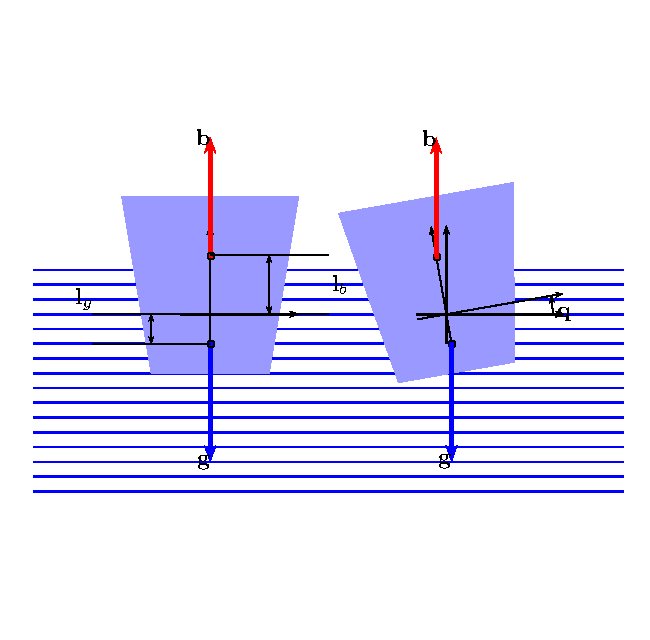
\includegraphics{ShipExample}
    \caption{The Floating Ship Example}
    \label{fig:ShipFloating}
  \end{center}
\end{figure}

The sway motion of the ship shown in Figure ~\ref{fig:ShipFloating} can be described by Equation~\ref{eq:shipflow}
\begin{equation}
\label{eq:shipflow}
J\ddot{q}+d\dot{q}=\tau(q)_{g}+\tau(q)_{b}+\tau_{u}
\end{equation}


where $q$ is the swaying angle,
$J$ is the inertia,  
$d$ is the damping coefficient,
and $\tau_{g}$,$\tau_{b}$,$\tau_{u}$ are the corresponding torques of gravity, buoyancy and external control.

When a ship is at sea, its motion is mainly governed by the two forces,  buoyancy $b$ and gravity $g$.
If $\tau_{u}=0$,  the ship motion is totally governed by the natural dynamic forces.
Such a system is \emph{autonomous}.

To make it consistent with the discussions in the following chapters, Equation~\ref{eq:shipflow} is reformulated.
By defining the \emph{state} variable $\state=[q,\qd]$,  Equation~\ref{eq:shipflow} becomes
\[
\dot{\state}=F_{J,d}(\state)+Du
\]

where 
$F$ is a function of $\state$, the subscripts~$J$ and~$d$ are \emph{system parameters},
$D$ is a matrix, which describes how the control effort is applied,
and $u$ is \emph{control input}.
For this example $u$ is $\tau_{u}$, which is $0$.



\subsubsection*{Equilibrium Postures}
A ship will only rest at the postures where $\tau_{g}+\tau_{b}+\tau_{u}=0$, which are called \emph{Equilibrium} Postures.
The only two possible ones are shown in Figure ~\ref{fig:ShipEqulibriumStable} and Figure~\ref{fig:ShipEqulibriumUnstable}.
\begin{figure}[!htbp]
  \begin{center}
     \includegraphics{leftPos}
    \caption{The Stable Equilibrium Posture}
    \label{fig:ShipEqulibriumStable}
  \end{center}
\end{figure}

\begin{figure}[!htbp]
  \begin{center}
     \includegraphics{rightPos}
    \caption{The Unstable Equilibrium Posture}
    \label{fig:ShipEqulibriumUnstable}
  \end{center}
\end{figure}



However, the two postures are different, which is illustrated with the \emph{phase plot}.
On the phase plot, the horizontal axis represents  $q$; and the vertical axis represents velocity $\qd$. 
On the phase plot, the motion of the ship is shown as a curve, which is called \emph{flow}.

The posture in Figure ~\ref{fig:ShipEqulibriumStable} is \emph{attractive} or \emph{stable}.
If a small perturbation moves the ship away from the left posture, it will return to the equilibrium posture automatically as shown in Figure~\ref{fig:StablePosture}.
\begin{figure}[!htbp]
  \begin{center}
      \includegraphics{stablePosition}
    \caption{Phase Plot of the Stable Posture}
    \label{fig:StablePosture}
  \end{center}
\end{figure}


Whereas the  posture in Figure~\ref{fig:ShipEqulibriumUnstable} is \emph{repelling} or \emph{unstable}, if the ship is moved away from the equilibrium posture,  by natural dynamics, it will move away even further, as shown in Figure~\ref{fig:unStablePosture}.

\begin{figure}[!htbp]
  \begin{center}
      \includegraphics{unstablePosition}
    \caption{Phase Plot of the Unstable Posture}
    \label{fig:unStablePosture}
  \end{center}
\end{figure}


\subsubsection*{A Simple Task}
All the flows form the \emph{phase portrait} of the dynamic system, which illustrates all the possible motions. 
The discovery is that all the flows start from the repelling posture and end at the attractive posture.
Several curves are shown in Figure ~\ref{fig:globalflow}.
This means that no matter what the current posture, the ship will return to the normal stable posture automatically.

This is an intrinsic property of natural dynamics, and thanks to this, balancing is a simple task which requires no control effort. 
This property is determined by the qualitative structure design criterion which demands the centre of buoyancy  is above the centre of gravity.

\begin{figure}[!htbp]
  \begin{center}
   \includegraphics[width=0.7\textwidth]{ShipGlobalFlow}
   \caption{Global Properties of the Flows: All the curves start from the repelling posture~(Red) and end at the attractive one(Blue)}
   \label{fig:globalflow}
  \end{center}
\end{figure}

 



\subsubsection*{Generalization of the Ship Example} 
This conclusion is independent of the shape, size, weight or material of the ship. 
In general cases, the same wave perturbation will result in different sway motions for different ships.
However, as long as the qualitative structure design criterion is maintained, balancing remains ``easy''.
The phase portraits of all  ships share following properties. 
\begin{itemize}
\item one repelling point 
\item one attractive point 
\item all flows start from repelling point and end at the  attractive point. 
\end{itemize}

In mathematical terms, all the phase portraits share the same topological structure of Figure~\ref{fig:topologyStructure}.

This phenomenon illustrates the principal idea of motion adaptation in {\moit}.
When the variations among individuals or situations result in motion variations, the qualitative dynamics or topological structure of the dynamic system remains invariant.

\begin{figure}[!htbp]
  \begin{center}
   \includegraphics{topologyStructure}
   \caption{the topology  the phase portraits of ship dynamic}
   \label{fig:topologyStructure}
  \end{center}
\end{figure}




\subsection{The Mass Spring System:  Symmetry Transformation}
Despite the complexity of the body structure, biological motor control is fast and accurate.
Such quantitative properties pose another puzzle in motor control research, as solving the complex dynamics directly would require prohibitively long computational time and excessive mental resources.

{\moit}\ proposes a new method to achieve speed and accuracy in motor control.
This efficient strategy is based on the ideas of transformation and symmetry.
New motions are achieved through transforming template motions,without solving the dynamics. 
To keep the motion natural looking, the control system chooses the transformation directions that are energy efficient, or using an alternative, allowed by the natural dynamics.


Such ideas can be illustrated by the following mass spring example, shown in Figure~\ref{fig:massspring}.
The mass spring system is selected because it captures some important properties of biological dynamics.
The compliant actuators of muscles work like springs, and rigid bones are modelled as mass.


\begin{figure}[!htbp]
  \begin{center}
    \includegraphics[width=0.7\textwidth]{MassSpring}
    \caption{the mass spring system}
    \label{fig:massspring}
  \end{center}
\end{figure}

\subsubsection*{Dynamics}
The canonical equation of a mass spring system is Equation~\ref{eq:mass-spring}
\begin{equation}
\label{eq:mass-spring}
\ddot{q}+q=0.
\end{equation}
where $q$ is the offset distance.

By defining the \emph{state variable}, $\state=[q,\qd]$, Equation~\ref{eq:mass-spring} can also be reformulated in the form as
\[
\dot{\state}=F(\state)
\]

Figure~\ref{fig:massSpringPhasePlot} shows two flows passing through different states $x$ and $x'$ on the phase plot.


\begin{figure}[!htbp]
  \begin{center}
     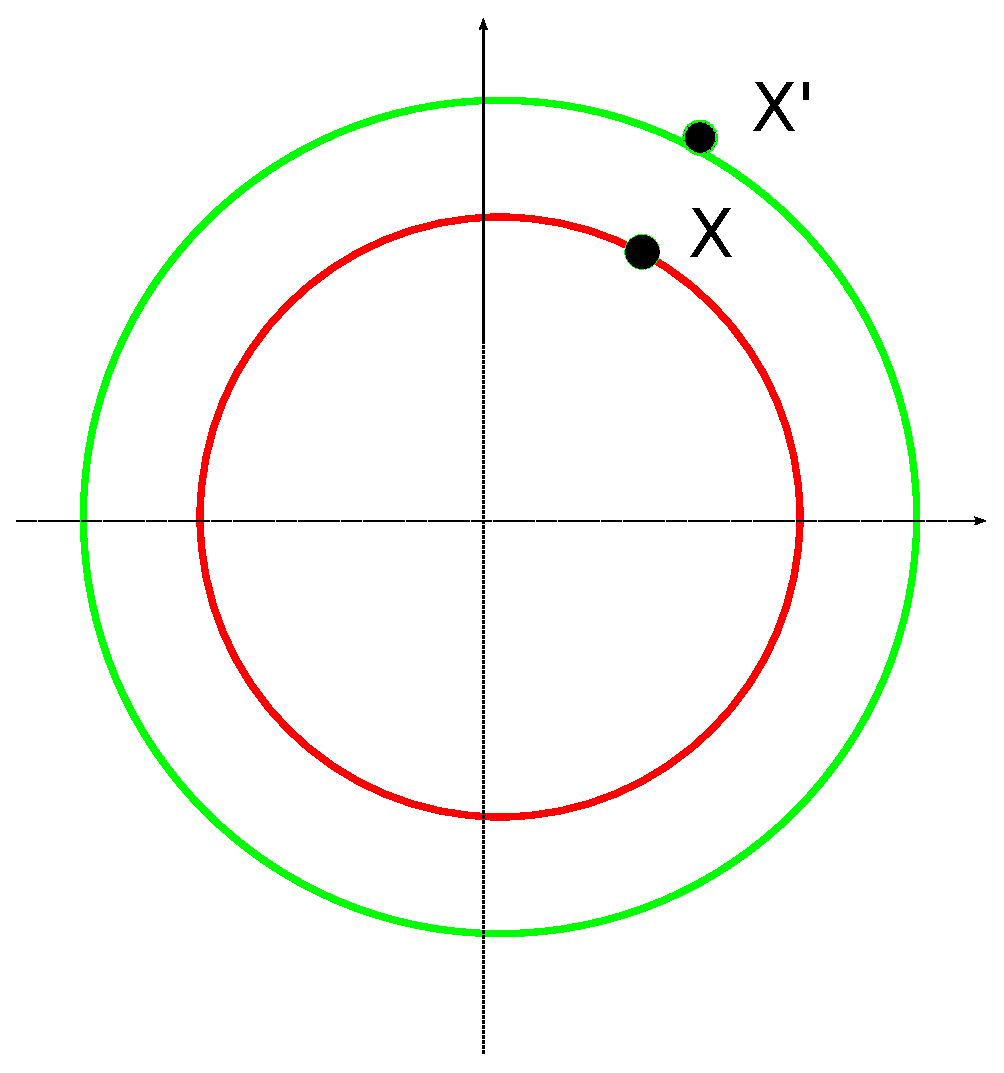
\includegraphics[width=0.5\textwidth]{MassSpringPhasePlot}
    \caption{Mass Spring Phase Plot: two flows pass through different states ($\state$ and ${\state}'$)}
    \label{fig:massSpringPhasePlot}  
  \end{center}
\end{figure}

\subsubsection*{Symmetry and Transformation}
%It is highly unlikely animals can solve Equation~\ref{eq:mass-spring}.

The mass spring system has some ``symmetrical properties''.
To an intuitive eye, different flows share the same circle ``Shape''.
Without solving the Equation~\ref{eq:mass-spring}, new flows~(solid ones) can be obtained by scaling the original~(red) flow.

From a mechanical viewpoint, this is because the flows of a mass spring system preserve energy.
To see this, we can define the energy function
\[
E=\frac{1}{2}(m\qd^2+kq^2)
\]
where $k$ is the stiffness, $m$ is the mass.
Since $E$ is a constant, we make $E=c$,
When $m=1,k=1$, we obtain
\[
 q^2+\qd^2=2c
\]
 
The equation above is the implicit function of a circle.

Therefore, given a template flow that passes through  $\state$, the flow passes through $\state'$  can be obtained by enlarge the original template flow.
In this manner, we determine the future motion after $\state'$, without solving the dynamics.


\subsubsection*{Dynamic Perception and Local Motor Invariant}

The idea of ``transformation and symmetry'' may shed light on the dynamic perception problem. 
It is highly unlikely that animals solve Equation~\ref{eq:mass-spring} to understand the the mass spring system.
As an alternative, the dynamics can be encoded in a different manner: a motion template and the symmetry property. 
If so, observed motions can be validated by checking them against our memorized motion templates.

To make it better, it is even unnecessary to work out the transformation.
In fact, it is enough just to check some property invariant under transformation.
For the example of mass spring system , we can check the ``shape'' of the flow.
For a mechanical perspective, this means to check the energy preserving property.

 
The invariant properties like preserving energy or shape can be quantitatively measured.
Since they are invariant only when flows move in a specific direction, they are called  \emph{Local Motor Invariant}. 


\subsection{Rimless Wheel}
The third example is a mechanical system with a more complex structure, the rimless wheel.
The complexity of the mechanical structure provides an opportunity to test various control ideas and compare them.

\subsubsection*{Dynamics}
The Simple 2D model is shown in Figure ~\ref{fig:rimlesswheel}. 
\begin{figure}[!htbp]
  \begin{center}
     \includegraphics[width=0.5\textwidth]{RimlessWheel}
    \caption{The Rimless Wheel}
    \label{fig:rimlesswheel}  
  \end{center}
\end{figure}
Where $\alpha$ is the angle between the spokes,  $\gamma$ is the angle of the slope,
$L$ is the length of the spoke,$\gv$ is gravity.

The dynamics of the system includes two phases: the rolling phase and the striking phase.

During the rolling phase, the rimless wheel works like a pendulum, the dynamics is as follows:
\[
\ddot{\theta}=\frac{\gv}{L}\sin(\theta+\gamma)
\]
When another spoke hits the ground, a strike happens. The impulse equation is
\[
\dot{\theta}=\cos(\alpha)\dot{\theta}
\] 

Comparing with the mass spring system, the motion of a rimless wheel is more complex. 
Depending on the initial condition, rimless wheel can roll uphill, roll downhill, stand with one spoke or stand with two spokes.
As the rimless wheel continues its motion, the final results of motion may be of any the following:
\begin{itemize}
\item rolling down the hill at a constant speed.
\item rolling down the hill at ever increasing speed.
\item stopping with one spoke as support.
\item stopping with two spokes as support.
\end{itemize}
The first one is of much interest.
In dynamics, constant rolling speed means the flow forms a limit cycle.
Figure~\ref{fig:lcofrimlesswheel} shows the limit cycle on a phase plot.
\begin{figure}[!htbp]
  \begin{center}
     \includegraphics[width=0.5\textwidth]{limitcycle}
    \caption{The Limit Cycle of The Rimless Wheel}
    \label{fig:lcofrimlesswheel}  
  \end{center}
\end{figure}




\subsubsection*{The Qualitative Approach}
The motion of a rimless wheel can be controlled by many methods.
The first method explores the topological invariant property.
For the rimless wheel system, the angle $\alpha$ between spokes and the slope angle $\gamma$ can be changed.
By doing this, we can change the constant rolling speed of the rimless wheel.
This will result in  a series of dynamic systems autonomous to the original one.
By gradually changing the parameter, on the phase plot, the limit cycle changes its shape accordingly.
The limit cycles of different mechanical parameters are shown in Figure~\ref{fig:morphyingrimlesss}

\begin{figure}[!htbp]
  \begin{center}
     \includegraphics[width=0.5\textwidth]{parameterchange}
    \caption{Different Mechanical Parameters result in Different Rimless Wheel}
    \label{fig:morphyingrimlesss}  
  \end{center}
\end{figure}



This is the qualitative approach; motion can be adapted by changing the parameter of the mechanical system. 
This method  requires no control energy input to maintain the new motion; it is energy efficient and easy to implement. 
However, the relationship between system parameters and the deformation of the limit cycle is hard to find, which prevents applying this method for tasks that require precision. 

For example, given a state on the state space, it is difficult to make limit cycle pass through the state by changing the parameters.

\subsubsection*{The Quantitative Approach}

Another approach control the rolling speed by applying control force.
For example, we apply control $u$ to the dynamic system, then the equation becomes
\[
\ddot{\theta}=\frac{\gv}{L}\sin(\theta+\gamma)+u
\]

if we set $u = \ep\frac{\gv}{L}\sin(\theta+\gamma)$, where $\ep$ is a parameter,
Then the rolling speed of the rimless wheel will be a parameter of $u$.
Figure~\ref{fig:timescalingrimlesswheel} shows two limit cycles of different $\ep$ parameter on a phase plot.
\begin{figure}[!htbp]
  \begin{center}
     \includegraphics[width=0.5\textwidth]{timescaling}
    \caption{Different Limit Cycles with Different Control}
    \label{fig:timescalingrimlesswheel}  
  \end{center}
\end{figure}

 As shown in Figure~\ref{fig:timescalingrimlesswheel}, the limit cycle is stretched vertically.
The relationship between $\ep$ and the rolling speed is simple, making this method computationally efficient and suitable for precise tasks. To make the limit cycle pass through a state $(\theta, \dot{\theta})$, if the state of same $\theta$ on the limit cycle is $ (\theta,\dot{\theta}’)$, then we have 
\[
\ep= (\frac{\dot{\theta}}{\dot{\theta}'})^2-1
\]

The disadvantage of this method is it require energy input.
Therefore for a large deformations,this method is not energy efficient.

\subsubsection*{The Difference and Comparison}
These two methods are different but related.
Neither methods will change the dynamics qualitatively. 
The systems after parameter modification,  or the controlled systems are still able to run uphill, down hill, stop with one or two spokes and roll at a constant speed.

This demonstrates the underlying topology is not changed.
Both methods try  to transform the phase portrait. 
The different transformation require different computational or energy cost.

There is another reason for choosing the rimless wheel as a example, its dynamics resemble that of animals' locomotion behaviour.
As further development, we propose this idea for motion control of dynamic characters.






\section{Contribution}

Compared with current \cms methods, the new approach has several advantages:
\begin{enumerate}
\HiItem {More Types of Adaptation.}
Most dynamic methods only focus on generating responsive motions to dynamic perturbations.
Adaptations across different characters are treated as an independent research topic~(motion re-targeting) and are tackled with very different methods.
{\moit}\ solves the two problems with one approach.
The mathematical idea of topological conjugacy  incorporates both motion re-targeting and  perturbation responses  in a unified framework.
Thus {\moit}\ is capable of more types of adaptation.
\HiItem {Better Usability.}
For many \cms methods, each \dof ~is controlled independently.
When modifying motions, the animator has to modify each \dof, which is tedious work.

In {\moit}, adaptation is achieved by applying transformation.
Each transformation can be parameterized by one parameter. 
By specifying only one parameter for the transformation, control inputs of all {\dof}s are modified automatically, making this method easier to use.

\HiItem {No Reference Motion Needed.}
{\moit}\ relies on the dynamics of body and environment.
Motion Capture Data are not needed as reference input.
In some situations, this method can generate new motion that cannot be captured.


\HiItem {Computationally Efficient.} 
This motion synthesis approach requires little computation time and memory, therefore it suits real-time applications.
\HiItem {Dynamic Motion Transition.}
Transitional motion can also be simulated dynamically, and in this research such methods have been developed upon solid theoretical foundation.

\end{enumerate}

Because of its biological foundation,
algorithms and simulation results of {\moit}\  might shed light on biology research questions.
Some conclusions and control techniques developed in this thesis provide alternative ideas for biological motor control, and have potential theoretical value.

\begin{enumerate}
\item 
The Motion Primitive Hypothesis is an old idea in biological research, but there is no agreement on the definition and underlying reasons.
Biological research has tried to identify motion primitives by exploring neural anatomy, EMG signals or muscle activation patterns.

{\moit}\ examines motion primitives from the dynamic viewpoint.
The discovery and conclusion are more logical and complete.
Besides pointing out a motion primitive, {\moit}\ also explains why certain motions become primitive, how many primitives exist, and how they are formed.


\item Many biological research ideas like \cpg and invariant based perception are proposed empirically. 
For a complete theory, much necessary detailed information is still missing.
As a contrast, {\moit}\ is based on rigid mathematical theory, for many biological ideas, {\moit}\ provides workable mathematical machinery.

\end{enumerate}







\section{Organization of the Thesis}

This thesis is organised as follows.
 
In Chapter~\ref{chap:background}, previous research on motion synthesis and biological motor control which are the motivation and justification for {\moit} are discussed, .
 
In Chapter~\ref{chap:gi},  \emph{The Qualitative Dynamics Theory} is introduced to explain motion primitives. 
Biological based  methods for maintaining the global motor invariant are developed.

Chapter~\ref{chap:li} focuses on the idea of Local Motor Invariant and Symmetry.
Lie Group Theory is  introduced  to analyse the symmetrical properties in motion dynamics.
Symmetry Controllers are developed to provide necessary energy input for adapting motions.
 


Chapter~\ref{chap:msf} discusses the combination problems.
For a single motion primitive,  strategies are developed to preserve both the global and local motor invariant simultaneously.
Motion primitive transition is discussed.
Methods for combining motion elements into more complex motions are developed.
Finally, in oder to develop an animation system, the software architecture and work flow are discussed.

Chapter~\ref{chap:gi},~\ref{chap:li} and \ref{chap:msf} lay down the theoretical foundation of {\moit}.
The following chapter provides experimental verification.



Chapter~\ref{chap:walk} focuses on the synthesizing adaptive motions for one primitive.
Bipedal walking,  which is commonly observed but poses great challenges for current \cms research,is chosen as the example,.
Methods based on {\moit}\ successfully boost the stability and generate adaptive gaits, and further validation shows the synthesized gaits comply with natural observation. 

In Chapter~\ref{chap:stance}, motion transition is discussed. 
A new balancing motion primitive is developed. 
Adaptive transitional motions from stance to walk and walk to stance are generated dynamically.


In Chapter~\ref{chap:highdor}, motor invariant theory is extended to more complex characters.
Three strategies are developed to simplify the problem for different situations.

This thesis ends with Chapter~\ref{chap:con}. 
After discussion of new finding arising from this research, some new questions and ideas for graphics and neural science are proposed for further research.





%%% ----------------------------------------------------------------------


%%% Local Variables: 
%%% mode: latex
%%% TeX-master: "../thesis"
%%% End: 


\section{Background and Previous Work}
\subsection{dynamic simulation}
Dynamic Motion Synthesis  tries to synthesize character motion through physical simulation of the mechanic structure of character body which is usually modelled as a linked rigid body system \cite{Baraff1994,Mirtich1996,Stewart2000}. Since many real physical properties are considered in the computation, the generated motion are normally physical feasible. However the most difficult task for those methods is to design a efficient control system to simulate the functionality of a real biological neural system. Some early research applied classical control methods like PD controller \cite{Raibert1991} for locomotion. Later research \cite{Hodgins1995} applied the same method for different tasks like running, bicycling, vaulting and balancing. Limit Circle Control(LCC) \cite{Laszlo1996} provides an alternative method for lower energy locomotion animation. However both the classical PD controller and Limit Circle Controller predefined motion trajectories and eliminated perturbations. This make them not good at generating motion adaptation.

Because lots of degrees of freedom are involved in the whole body simulation, in most cases, motion solutions are not unique. Many optimization methods have been applied to choose the ``best'' motion. For dynamic methods, a reasonable choice is to minimize the energy cost~$V$, such that 
\[
\textbf{V}=\int_{t0}^{t1}F_{a}(x)^2dt
\]
where $F_{a}$ is the active force generated by actuators like motors or muscles. This is introduced to CMS research as the influential Spacetime Constraints\cite{Witkin1988}, and serve as the foundation for many modern CMS research. \cite{Jain2009} provides an example for locomotion;  \cite{BalanceControl} find a method for balance maintaining movement. \cite{Liu2009} proposed a method for object manipulating animation.

\subsection{Optimizaiton Based Method}
Optimization provided an idea for solving the redundant freedom problem and complies with energy efficient principle of natural motion.  But this method has several drawbacks for motion synthesis application.
(1) Numeric Stability and Modelling Difficulties
Optimization method only grantee the energy efficiently of the motion, but nothing is about the converging speed and stability. Even the optimal solution is natural looking, it is very hard find.
it can obtain the solution when the model is accurate and the initial guess is near the optimal solution.
So this method is sensitive to model error and initial condition. 
While for motion, the accurate model is very hard to achieve and artefacts are generated.
Liu2005  points out that spacetime constraint methods only suit high energy motions like jumping and running; for low energy motion tasks like walking the result doesn't looks nature. This is mainly because the muscle effects are neglected.
(2) Computational Complexity
Motion Control is variational problem in nature. For complex body structure, even the state of art numeric method will take inhibitive long time. And little is know about how to reuse the computation result for motion adaptation.
(3) Limited Application Domain
Optimization method nowadays only applies for very limited motion. Main for motion can by model with rigid body.
 A Large of motion are still uncovered. Like heart beating, breathing, fish swims and bird flying, such motion involves the soft body and fluid dynamics. Such model are computational difficult in nature, apply optimization based method for such dynamic are not computational feasible.
2.1.2 motion perception problem
For motion synthesis research in Graphics, we focus on generating natural looking motion rather than physically-correct motion. As long as the audience don’t notice the artefacts, such result will be OK. A important biological question is how human recognize motion and detect the artefacts. Natural looking motion observed from life must be physically feasible, but it does not mean human detects motion artefacts by doing physical calculation in mind for the speed limitation, nor it is only because memory of motion for the capacity limitation.
\subsection{Limit Circle Based Method}
\subsection{Motion Primitives}
2.2 The Lessons from Biology Research
Motor Control from biology research is full of paradoxes.
Motor Control in nature is a very complex process, it involves electrical, chemical and mechanical changes. However, for such complex problem, seems an easy task for most human and animals.
From biological view port, the problems of optimization are worse. Natural motor control faces many limitation of the biological motor control system
2.2.1 Biological Constraints
(1) Sensing and Control Limitation
Motor control is not only a mechanical problem, it is a complex process. For the biological system,  many crucial parameters and variables are not accessible. Dynamic model, force, torque, angle can only sensed with approximation, while mass, inertia, and human have not direct sense. For some control variables like toque, neural system has no direct control access.

Besides this, body and environment is noise and time varying.
Methods are sensitive to errors are not suitable for biological motor control.

(2) Neural Computation
The neural system is powerful but it is inferior in speed and accuracy when compared with digital computer. Neural signal transmitting speed is slow; and there is a long delay between neural signal firing and force generation in muscles. It is impossible for neural system to carry out complex computation for optimization in real-time time.
2.2.2 Biological Discoveries
Limited Computation Activity
Common Life experience shows motor control maybe an easy task. This is proved by some biological research. Many experiments show motion can happen even without brain input.
Development
Many motor ability are born, rather than developed. Eating, Breeding, Breathing and locomotion, many motor ability in animals seems is inborn rather than learned. 
Evolution
Form Evolution view port, the motion style seems not close related to the development of neural system. Wales and Fishes swim in a similar manner.
What is apparent is the body and environment. Animals with a similar body in a similar environment usually move in similar manner.
2.3 Different Biological Motor Control idea
Biological Research propose some different idea about motor control, which takes the biological constraints into consideration.
 equilibrium point hypothesis and uncontrolled manifold hypothesis
An idea of motor that will simply the computation and maintain the energy efficiency is eph and ump. Some proposed that neural system doesn’t control all the system,  it may only control the final motion result. As long as the motion finish its task, it don’t matter how it is carried out.
This means control final motion position, and let motion move freely according to the environment and body condition. Which should be computational efficient and energy efficient.
 morphological computation and motion primitives framework.
Animals don’t move the way they want, but only the way they can.
It is the body and environment plays the most important role in motor control, they forms the basic pattern of motion, neural system only tuning or tweak the basic pattern to fit animal’s special needs.
More complex motions are based on combine the basic pattern together.
This idea is easy to compute and can provide a way for motion perception.
Basic pattern are limited and human are very familiar. When the pattern is break, human will notices the difference will result motion artefacts.
2.4 The relationship between our research and new ideas
There is no a unified way to identify motion pattern and motion primitives. In our framework, we based on the idea of group and invariant.
Motion Primitive in our eyes is the global qualitative properties of motion, which is capture by the topology structure of the dynamics of body and environment. This is the Global Motor Invariant.
EPH are adopted as a method for tweaking basic pattern. The method we propose for equilibrium point control is based on symmetry properties of differential equation. This is the Local Motor Invariant.
Because our method is based on dynamics, so it is physically-based method. The advantage of Goup and Invariant theory is that it will provide an efficient computational method.
\chapter{GLOBAL MOTOR INVARIANT}
\label{chap:gi}
\section{Introduction}

\nomenclature{$q$}{Generalized Coordinates}
\nomenclature{$Q$}{Configureation Space or Configuration Manifold}
\nomenclature{$\qd$}{Gneralized Velocity}
\nomenclature{$TQ$}{Tangenet Bundle of $Q$}
\nomenclature{$u$}{Control Input}
\nomenclature{$\state$}{State Variable}
\nomenclature{$M$}{State Space Manifold}
\nomenclature{$TM$}{Tangent Boundle Manifold}
\nomenclature{$A$}{Attractor}
\nomenclature{$B(A)$}{Basin of Attration of $A$}
\nomenclature{$S$}{Neural Oscilator}
\nomenclature{$\uin$}{Input Signal to the Neural Oscilator}
\nomenclature{$\uout$}{Output of the Neural Oscilator}
\nomenclature{$\hin$}{Input Coefficient of the Neural Oscilator}
\nomenclature{$\hout$}{Output Coefficent of the Neural Oscilator}
\nomenclature{$\simeq$}{Topology Conjungacy}


%\nomenclature[zcif]{$CIF$}{Cauchy's Integral Formula}                                % first letter Z is for Acronyms 
%\nomenclature[aF]{$F$}{complex function}                                                   % first letter A is for Roman symbols
%\nomenclature[gp]{$\pi$}{ $\simeq 3.14\ldots$}                                             % first letter G is for Greek Symbols
%\nomenclature[gi]{$\iota$}{unit imaginary number $\sqrt{-1}$}                      % first letter G is for Greek Symbols
%\nomenclature[gg]{$\gamma$}{a simply closed curve on a complex plane}  % first letter G is for Greek Symbols
%\nomenclature[xi]{$\oint_\gamma$}{integration around a curve $\gamma$} % first letter X is for Other Symbols
%\nomenclature[rj]{$j$}{superscript index}                                                       % first letter R is for superscripts
%\nomenclature[s0]{$0$}{subscript index}                                                        % first letter S is for subscripts



\ifpdf
    \graphicspath{{GlobalInvariant/GlobalInvariantFigs/PNG/}{GlobalInvariant/GlobalInvariantFigs/PDF/}{GlobalInvariant/GlobalInvariantFigs/}}
\else
    \graphicspath{{GlobalInvariant/GlobalInvariantFigs/EPS/}{GlobalInvariant/GlobalInvariantFigs/}}
\fi

Motion varies greatly, different people walk with different gait. 
A question is why the different motions of different people are all called walk.
Our answer is walk is not determined by the details how it is carried out.
Walk capture the qualitative properties, and we agree on the walk becomes it is a property encoded in all our body, we all have the walking ability inborn, so that’s the reason why we can all identify it.


Our basic idea is motion primitives are ''easy'' to finish. 
In this chapter, we will try to give the “easiness” definition.
The biological ideas can be provide a clear mathematical meaning.


\section{Basic Concepts of Qualitative Dynamics}
This section develops the mathematical conceptualization of Global Motor Invariant.
Some mathematical background is needed in this discussion.
Throughout this paper, we take the geometrical viewport of mechanical system.
For analyzing qualitative properties, we introduce the ideas from differential topology.
This idea can be traced back to Poincare\citep{Poincar'e1899,Poincar'e1885} and recently developed by the Smale School\citep{Smale1970}.
It is impossible to put the a whole discipline in one chapter.
Please refer to other books and lectures such as \citep{abraham1978foundations}for introduction in details.


Dynamic motions are modelled as differential equations,
In the geometrical viewport, differential equation describes a differentiable manifold.
Qualitative Properties can be obtained by analyzing the topological structure of the differentiable manifold.
Global Motor Invariant is defined by the topology structure.



\subsection{Dynamic System and Differential Manifold}



The dynamic of a mechanical system is determined by its configuration  $q$ and generalized speed $\qd$. 
we represent the state of a system as a vector $\state=[q,\qd] \in M$,  $M$ is the state space, or state manifold.
The motion is a trajectory $t \mapsto q(t)$ in the configuration space parameterized by time~$t$.
For a dynamic system, $q(t)$ usually is derived from the state trajectory $\state(t)$, which is described by differential equaiton. 


For every point $x \in M$, 
$F$ and $u$ determines a derivative vector $\dot{x} in T_{x}M$ in the Tangent Space. 
All the vectors over the full space of $x$ form the \textbf{vector field} $\mathbf{V}$,describe by the differential equaiton~ \ref{eq:ode}
which described by the differential equation
\begin{equation}
\label{eq:ode}
\dot{\state}=F_a(\state,u),\state\in M
\end{equation}

where $u$ is the control effort. 
$a$ is the system parameters
$F$ is determined by the system's natural property.
If $u=0$,  no control effort is applied.
Such systems are \textbf{autonomous systems}. 

By solving the \textbf{intergral curve}to equation~\ref{eq:ode}, 
\textbf{flow} $\Phi(\state)$ of $\mathbf{V}$ is the \textbf{intergral curve} through $\state$. 
all the flows form the \textbf{phase portrait}, which illustrates all the possible motions of the dynamic system.
We usually visualize the differential manifold by \textbf{phase plot}.


An illustrative example repeatedly used in this report is the mass-spring system. 
After linear transformation,  
a linear mass spring system can be described in canonical form equation ~\ref{eq:mass-spring}
where $q$ is the position of the mass, $\qd$ is the speed, and $\ddot{q}$ is the acceleration of mass.
 
If we chose the state variable $\state=[q,\qd]$, the ODE model should be in the form of equation~\ref{eq:stateform}
\begin{equation}
\label{eq:stateform}
\dot{\state}=
\left[ 
\begin{array}{cc}
0 &1\\
-1 &0 
\end{array}
\right]\state
\end{equation}



\subsection{Global Motor Invariant}
Flows can only intersect at some special position called \textbf{equilibria}.
Basically there are three type of equilibrium.
At each \textbf{equilbria}, 
the local space can be divided into three subspace of sub manifold: centre sub manifold, stable manifold, and unstable sub manifold.
\begin{description} 
\item[centre sub manifold]
If a flow $\phi$ pass through a point $\state_{c}$ on centre sub manifold $W_{c}$,
flow$\phi$ will remain on the Centre Manifold 
\[
\phi_{c}(t) \in W_{c}, t \in R
\]
 An equilibria must be on center manifold. 
\item [stable sub manifold]
For the flow $\phi_{s}$ passes through a point $\state_{s}$ on stable sub manifold $W_{s}$, the flow will finally converge to a no wandering point on centre sub manifold.
\[
\phi_{s}(+\infty)=\theta_{c}
\]
\item[unstable sub manifold]
For the flow $\phi_u$ passes through a point $\state_u$ on unstable sub manifold $W_{u}$, the flow will be repelled from the no wandering points on centre manifold.
An alternative perspective is the inverse of the flow converge to no wandering point. 
\[
\phi_{u}(-\infty)=\theta_{c}
\] 

\end{description}

The size and dimension of each sub manifold varies.
For some cases, the $W_{s}$ ( $W_{u}$) may not exist, 
this can be seen as the dimension of $W_{s}$($W_{u}$) is $0$.
\textbf{Attractors} are the equilbria where the whole local space is stable, the dimension of unstable submanifold is zero $\mathbf{dim}(W_{u})=0$.
\textbf{Repellors} are the equilibrias where the whole local space is unstable,the dimension of stable submanifold is zero $\mathbf{dim}(W_{s})=0$.







In theory, only observe the attractor of the dynamic system can be observed, motion task should be only rely on the attractor.
Two types of attrator are of great interest in motor control:(1) fixed point, as show inf Figure~\ref{fig:StablePosture},(2)Limit Cycle,as shown in Figure ~\ref{fig:limit_circle}

\begin{figure}
\begin{center}
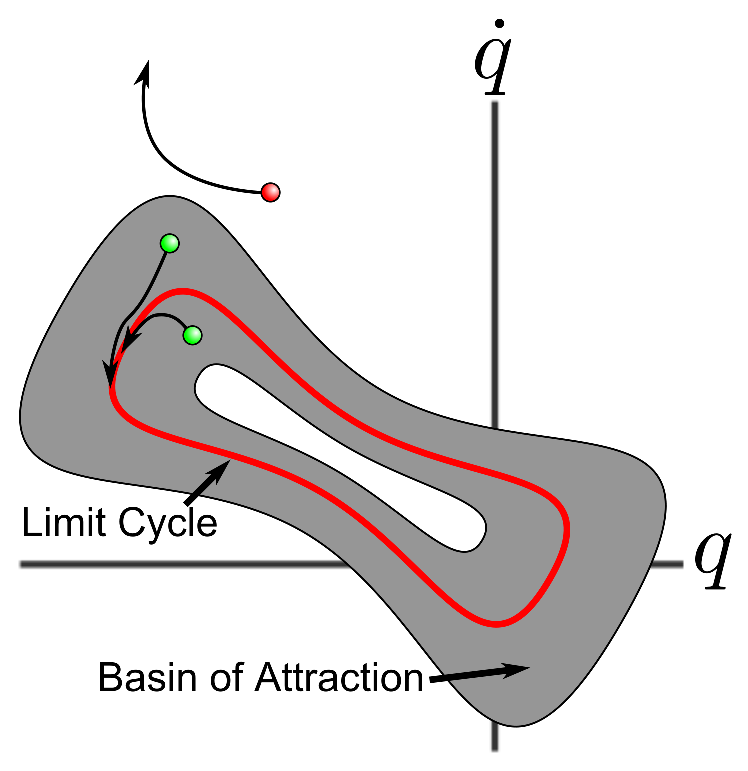
\includegraphics[height=0.4\textheight]{phase_plot}
\end{center}
\caption{Limit Cycle}
\label{fig:limit_circle}
\end{figure}




For nonlinear system, globally, the shape of stable and unstable sub manifold may be bending and connect with itself or each other.
The unstable manifold of one equilibrium may be the stable sub manifold of another.
The equilibra and its connectivity sub manifold form a topological structure.
Thus the phase plane will be divide into different regions,result in a cellular structure.
there is only one attractor, all the flow in this region will converge to the attractor ~$A$.
and the corresponding region is called basin of attraction ~$B(A)$.
as shown in figure~\ref{fig:manyboa}
\begin{figure}
\begin{center}
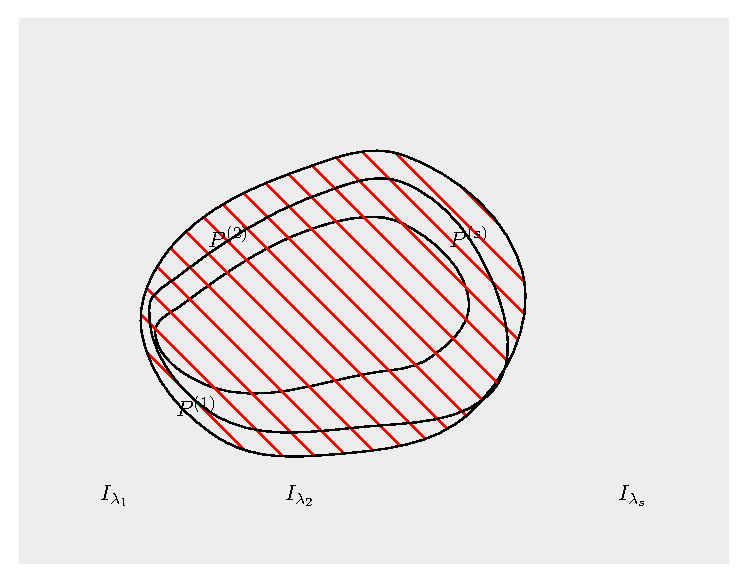
\includegraphics[height=0.4\textheight]{basinOfAttraction}
\end{center}
\caption{Celluar Structure of Phase Space}
\label{fig:manyboa}
\end{figure}


We can also give the biological ideas clear mathematical meaning.
The UMH, the uncontrolled manifold is the basin of attraction.
For EPH, the equilibrium point is the attractor.
For Impendence Control, impedance control is control the shape of basin of attraction.

\subsection{Analogous System And Topology Conjugacy}
many dynamic system are have different dynamic equation, but they share the same topology.
an example is the mass-spring system and the duffine system, described by equation ~\ref{eq:fuffin}
\begin{equation}
\label{eq:duffin}
\ddot{q}+q+q^{3}=0
\end{equation}
and the phase plot of the two system are show in figure~\ref{fig:msphaseplot},\ref{fig:duffin}

\begin{figure}
\begin{center}
\includegraphics[height=0.4\textheight]{massspring}
\end{center}
\caption{Mass Spring System}
\label{fig:msphaseplot}
\end{figure}

\begin{figure}
\begin{center}
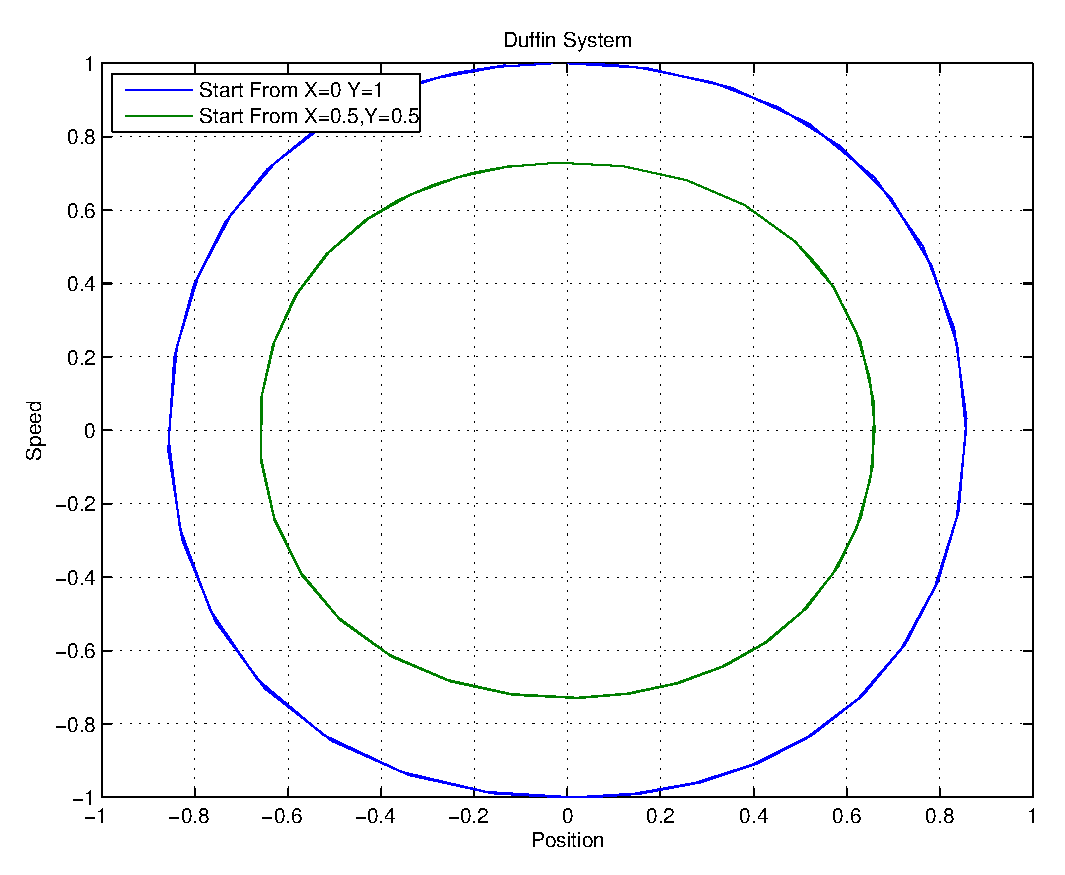
\includegraphics[height=0.4\textheight]{duffin}
\end{center}
\caption{Duffin Phase Plot}
\label{fig:duffin}
\end{figure}


one phase plot, the two system are similar, and we cand '' deform '' one into another.
in mathematical term, there is an equilalence relationship  for the two system. the \textbf{topological conjugacy}.

Let $X$ and $Y$ be topological spaces, and let $f\colon X\to X$ and $g\colon Y\to Y$
be continuous functions. We say that $f$ is
\emph{topologically semiconjugate} to $g$, if there exists a continuous
surjection $h\colon Y\to X$ such that $fh=hg$. If $h$ is a homeomorphism,
then we say that $f$ and $g$ are \emph{topologically conjugate}, and we call
$h$ a \emph{topological conjugation} between $f$ and $g$.



if two system are topological conjugate, they are analogous systems





\section{Global Motor Invariant and Motion Adaptation}
Global Motor Primitive is defined by the attractor type and its basin of attraction in the topology space.


Motion adaptation because of different reasons and in different situations.
Such two kinds of perturbation are treated separately and result in differentiation strategy or control.

\begin{itemize}
\HiItem{State perturbation}

The perturbation that move the state off the attractor is called State Perturbation, for only the state is changed, the dynamic system underline is not changed.


If the state is in the basin of attraction then, it will converge to the attractor. 
Start from different state position, it will result different flows, thus different motion.

Such kind of motion adaptation is called Responsive Motion Adaptation.
Because usually, for characters, perturbation comes from the push or pull, while the character and environment is not changed.

To make the character more responsive without result in motion failure,
Motion controller should try to enlarge the basin of attraction.






\HiItem{Structure Perturbation}

Another type of Perturbation will affect the dynamic system; such kind of perturbation is called Structure Perturbation. 
Such kind of perturbation happens commonly in our daily life, when a man put a heavy box on his shoulder, it will result a change in the dynamic system.

Structural Perturbation will change the phase portrait; some perturbation will make the system into an analogous system.
As a result, the even the current state is on the attractor, motion will change, this kind of motion adaptation is called system adaptation, and one important application is dynamic motion retargeting, when you change the character, the dynamic system changed.

Sometimes it will change the topology the underlying dynamic system, such effects are called bifurcation.
an example is the damping effects on the mass spring system.
as show in figure~\ref{fig:dampmass}

\begin{figure}
\begin{center}
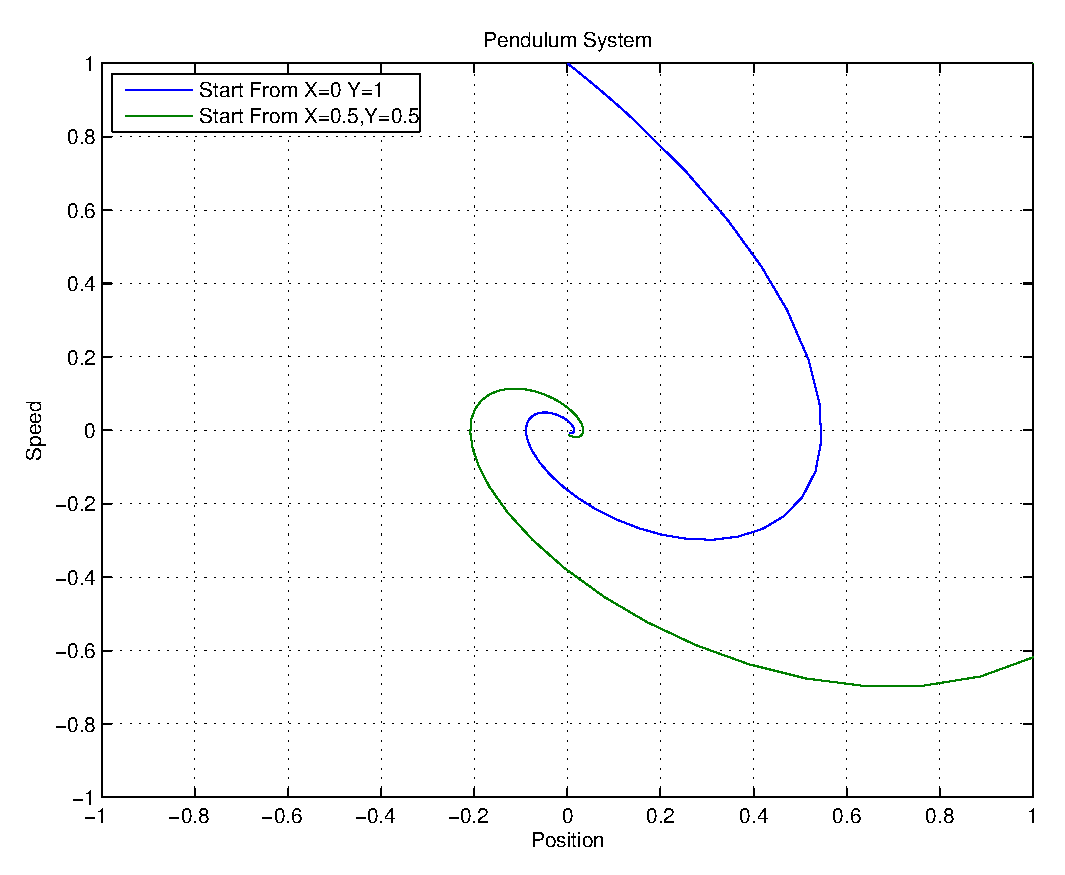
\includegraphics[height=0.4\textheight]{spring_damping}
\end{center}
\caption{damping perturbation onmass spring system}
\label{fig:dampmass}
\end{figure}

If ability of a dynamic system maintains its topology structure is structural stability.
To make characters more adaptive to environment and body change, motor controller should boost the structural stability of the motion.
Control effort should be prevent bifurcation.
\end{itemize}


\subsection{remarks on biological motor control}
Structural Stability is neglected in CMS research.
It is reasonable for natural animals to rely on structural stable autonomous system. 
In natural environment, perturbation and uncertainty are everywhere. In many cases, if neural system
can’t respond quickly enough, the better solution is to select a more structure stable motion primitives.

Structural Stability and Qualitative Idea provides a better explanation for some motion phenomena than quantitative theory like optimization and feedback shooting.
Qualitative Control Theory may help us understand the evolution of locomotion and neural Control.
Animals shift from the sea to the land. From quantitative computing viewport, the natural dynamics of the body and fluid environment are hard to predict or compute precisely. From the qualitative viewport, fluid is continuous
and uniform, the topology structure is very simple and stable, thus with little neural control fish can maintain its posture. On the other side, for human walking, although the rigid like
Environment can be calculated precisely, the topology structure is much more complex. 
Onthe phase plane, there exist many equilibrium points, the topology structure is more complex and unstable. 
The control system has to be more complex to control the more complex qualitative properties.

Qualitative theory can also help to explain another fact of biological motion system. 
Animals that live in similar environment and moves in a similar manner usually have similar body structure, in spite of their different position on evolution chain. 
This is because animals moving in a similar is based on the same motion primitive, similarity in body structure promise the topologial conjugacy.

This idea may help us to understand the body and environment effect in morphological computation theory. 
For specific environment, body evolves to provide us with a structural stable dynamic system, thus save lots of control effort for neural control.

We can also know motion primitives are not only defined by the body, it also defined by the environment, for motion in a specific environment, the topology should be fixed, thus the number of motion primitives is quite limited.


\section{Global Motor Invariant Control}
\subsection{CPG and Entrainment}
In nature, an animal's body and environment can be extremely complex. 
It leads to high dimensional manifolds with complicated topological structure, which provides many motion primitives for our use.
For CMS application, one question we want to ask is the so many motion primitives can be controlled with a simple method.

We propose that even there are many type of motion primitives, the type of attractor is limited. Basically there are only two types of attrator, limit circle and fix point.
Even the dimension of dynamic system maybe large, the dimension of the attrator is known. 
For fix point, its attractor is of dimension zero.
For limit circle, it is of dimension one.
Thus we can only focus on the type of attractor.



Biology Research suggested that the motor is mainly controlled by the Central Pattern Generator, which is a small autonomous network that generating rhythmic signals.
The idea of control motion by rhythmic signals can be modelled as entrainment \citep{Gonz'alez-Miranda2004}.
When coupling two oscillation system together, entrainment can happen when two system oscillator in synchronize. 
This effect will enhance the oscillation and also know as resonant. 




In previous section, we discussed two types of attractors: Fixed point and Limited Cycle. 
It is a still open question which type is more important and serve as the foundation as motor control\citep{Degallier2010}.
One idea limit circle is a necessary, fix point can be controlled with by 
(1) terminate a circle, 
(2)a different controller, 
(3)approximate by a limit circle with small amplitude or damping the limit circle, 
(4) change the limit circle into a fix point through by bifurcation. 



In this paper, 
\begin{itemize}
\HiItem Periodic behaviour is very common in biological systems. 
Besides the periodic motion in swimming and running, heart beating, wake and sleep also show periodic behaviour.
A periodic system has the potential to integrate with other bio system simulation to explore other motion features.

\HiItem Periodic motion has the same effect of terminated motion when the amplitude of limited circle is very small. 
For CMS research, both type of motion trajectory can be simulated with periodic motion.

\end{itemize}

\subsection{Neural Oscillator Stability}


Although it is difficult for neural system to carry out complex computation, it is easy to build oscillator structure with neurons. 
It only needs two neurons with mutual inhibitive property.
One extensively studied oscillation model is developed by \citet{neurooscillation}. 
The mathematical presentation is as follows:
\begin{eqnarray}
\tau_{1} \dot{s_{1}}&=&c-s_{1}-\beta l_{1}-\gamma [s_{2}]^{+}-\sum_{j}h_{j}[w_{j}]^{+}\\
\tau_{2} \dot{l_{1}}&=&[s_{1}]^{+}-l_{1}\\
\tau_{1} \dot{s_{2}}&=&c-s_{2}-\beta l_{2}-\gamma [s_{1}]^{-}-\sum_{j}h_{j}[w_{j}]^{-}\\
\tau_{2} \dot{l_{2}}&=&[s_{2}]^{+}-l_{2}\\
y_{i}&=&\mbox{max}(s_{i},0)\\
y_{o}&=&=[s_{1}]^{+}-[s_{2}]^{+}=y_{1}-y{2}
\label{eq:matsuta}
\end{eqnarray}

$c$,$\beta$,$\gamma$ are parameters of the oscillator,in our research are kept constant.
$\tau$ constrolls the oscilation frequency.







Matuoka oscillator is an autonomous oscillator; 
it can begin to oscillator without any control effort.
Figure ~\ref{fig:natural-oscilation} shows the natural oscillator output.
\begin{figure}[h]
\includegraphics[height=0.4\textheight]{oscillation.eps}
\caption{Natural Oscillation}
\label{fig:natural-oscilation}
\end{figure}





It is also adaptive; entrainment behaviour can happen between one Matuoka oscillator and different oscillators. 
Figure \ref{fig:entraint-oscilation} shows the entrain oscillation,
where the oscillation of Matuoka oscillator synchronise with the input signal.
\begin{figure}[h]
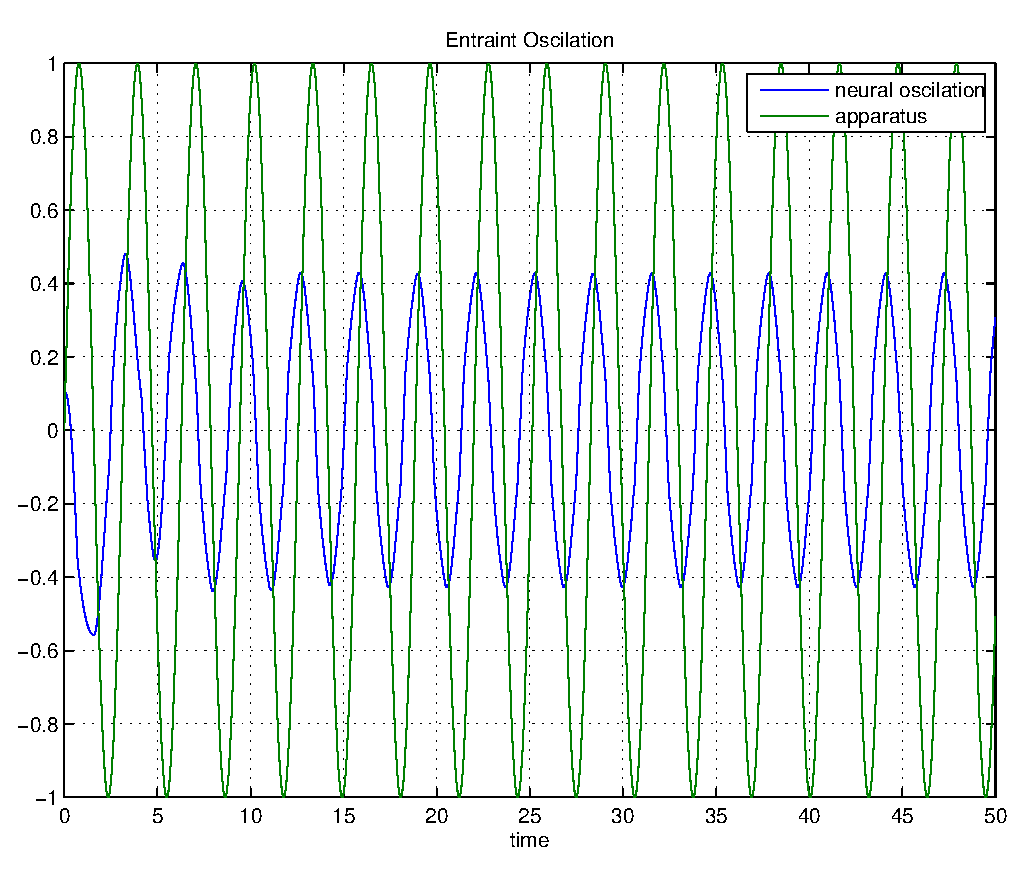
\includegraphics[height=0.4\textheight]{entraint_oscilation.eps}
\caption{Entrainment Oscillation}
\label{fig:entraint-oscilation}
\end{figure}

But because of the nonlinear properties, its behavior is not completely understood. 
Matsuta\citep{Matsuoka1987} explains the adaptive properties from the location of the roots of  characteristic equation. 
Wilimas\citep{Williamson1998} explains the properties in frequency domain.



In our research, we find some important properties of neural oscillator by empirical.

\begin{figure}
\begin{center}
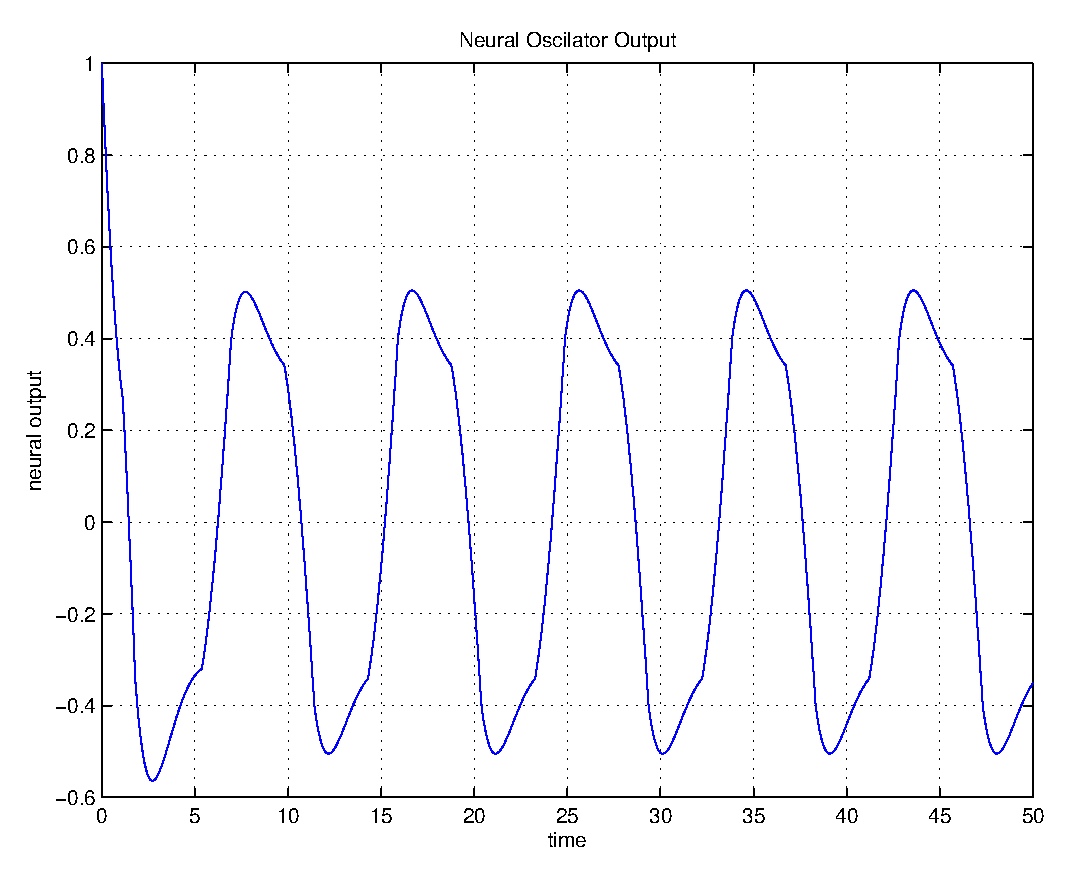
\includegraphics[height=0.5\textheight]{neuraloscilation1.eps}
\end{center}
\caption{The states of neural oscillator over Time}
\label{fig:oscilation}
\end{figure}

\begin{figure}
\begin{center}
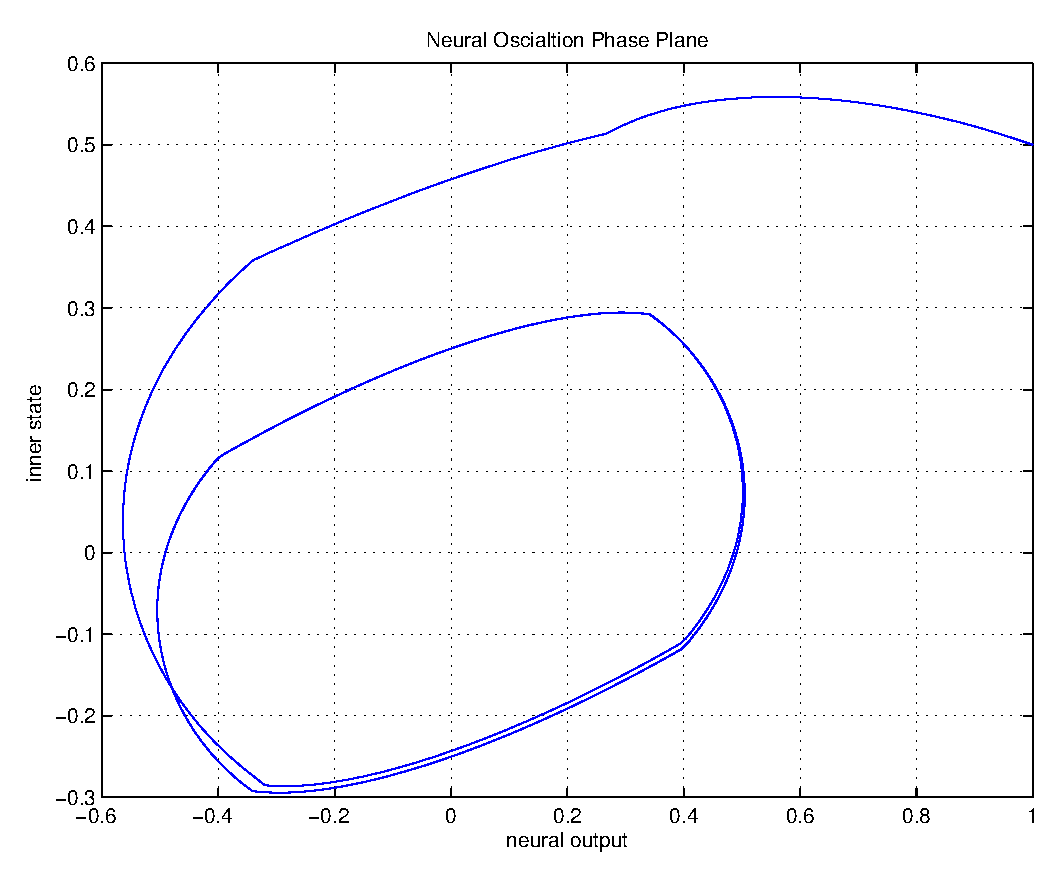
\includegraphics[height=0.5\textheight]{neural1phase.eps}
\end{center}
\caption{The phase portrait of Neural Oscillators}
\label{fig:oscilationphase}
\end{figure}

From our simulation, we investigate the topological structure.
Basically, neural oscillator shows three important properties:
\begin{itemize}
\item{Simple Topological Structure.}
The topology structure of neural oscillator is simple, 
it includes one  attractive limit circle and one fix repellor.
\item{Large Basin of Attraction.}
All the simulations we carried out converged to the same limited circle.
\item{Fast Converging Speed.}
In most of the case, the flow will converge to the limit circle within one period time.
\end{itemize}

Features above are shown in Figure ~\ref{fig:time_timeAttraction}.
\begin{figure}
\begin{center}
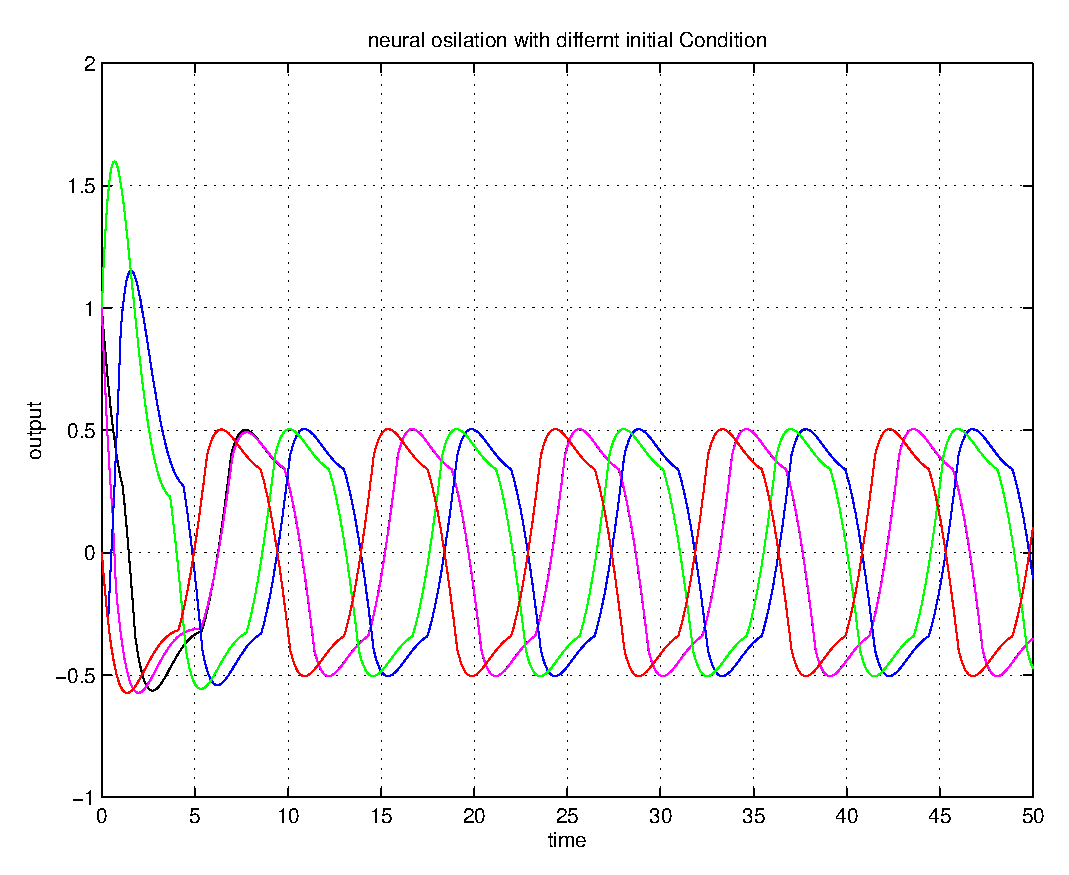
\includegraphics[height=0.4\textheight]{neural_attraction.eps}
\end{center}
\caption{Neural output with different initial position}
\label{fig:time_timeAttraction}
\end{figure}

\begin{figure}
\begin{center}
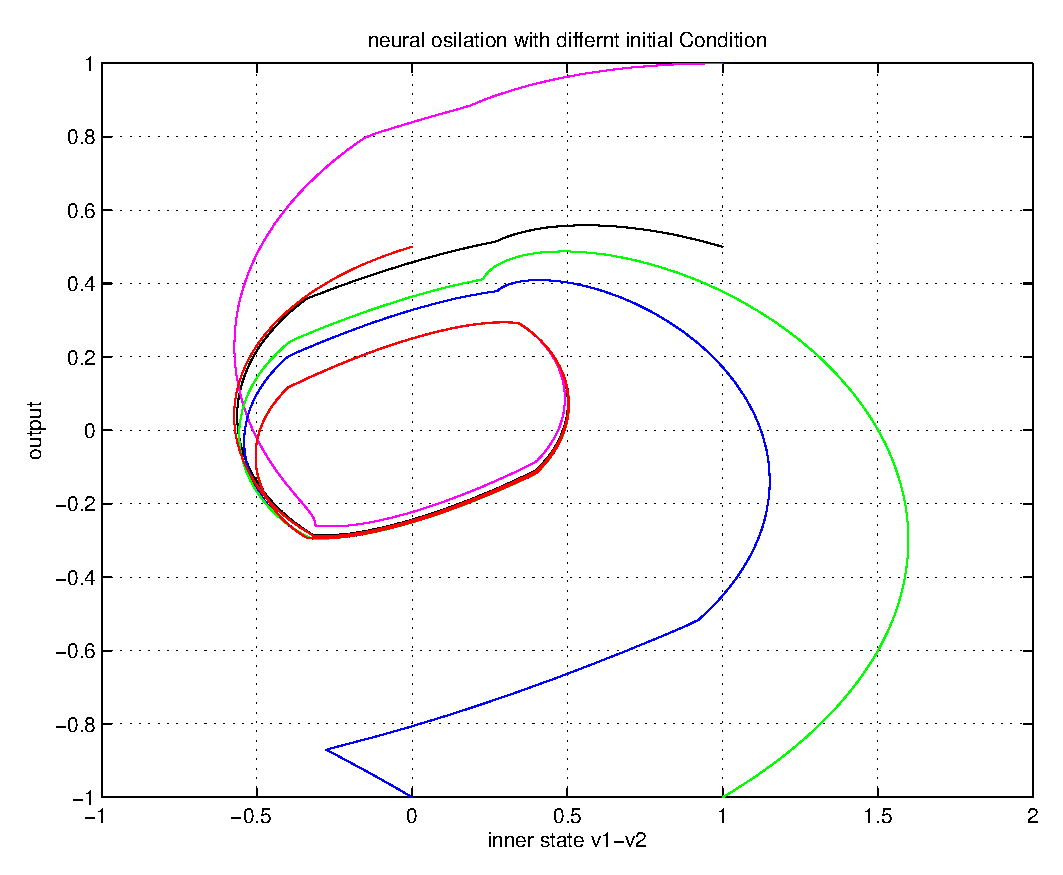
\includegraphics[height=0.4\textheight]{neural_attraction_phase.eps}
\end{center}
\caption{Phase plot of oscillation with different initial condition}
\label{fig:phase_attraction}
\end{figure}
 
The large area of basin of attraction means the final behaviour is totally determined by parameters. 
Initial condition will have no effects on the oscillator final output. 
Thus we treat matsuta oscilator as in a simple one input, one out put system, controlled by three parameter and input signal. 
we usually reformed equation ~\ref{eq:matsuta} in the simplified form
\begin{equation}
\label{eq:simplematsuta}
\uout=S_{[\hin,\hout,\tau]}(\uin)
\end{equation}
where $\uin=\sum_{j}h_{j}[w_{j}]=hw$,$\uout=\hout y_{o}$





The converging speed can be seen as quick recovery ability.
When an impulse perturbation happens, it will recover in one period time.


\section{Example:Maintain Bouncing Height}

Bouncing ball is system ball bouncing by moving a pedal, a system with simple dynamic but difficult to control with optimizaiton or pd. 
While this example capture the complexity of human interatction with the environment and object. 
And can be the basic model for many motion tasks.

We show in this example how neural oscillator can turn the bouncing ball system into motion primitive.
\subsection*{Dynamics}
Hybrid dynamics, in incoperate two phase, 
 

\begin{align}
\ddot{q}&=-g&\mathrm{if}\,\,q &> 0\,\,\mathrm{(free\,\,flying)} \nonumber\\
\dot{q}^{+}_{\mathrm{ball}} - \dot{q}^{+}_{\mathrm{paddle}} &=  \epsilon(\dot{q}^{-}_{\mathrm{ball}} - \dot{q}^{-}_{\mathrm{paddle}})&\mathrm{if}\,\,q &\leq 0\,\,\mathrm{(paddle\,\,strike)}\nonumber
\end{align}

Basically, the ball will continue bouncing with smaller height,as show in Figure~\ref{fig:bborg}.

\begin{figure}[h]
\begin{center}
	\subfigure[state plot]
	{
	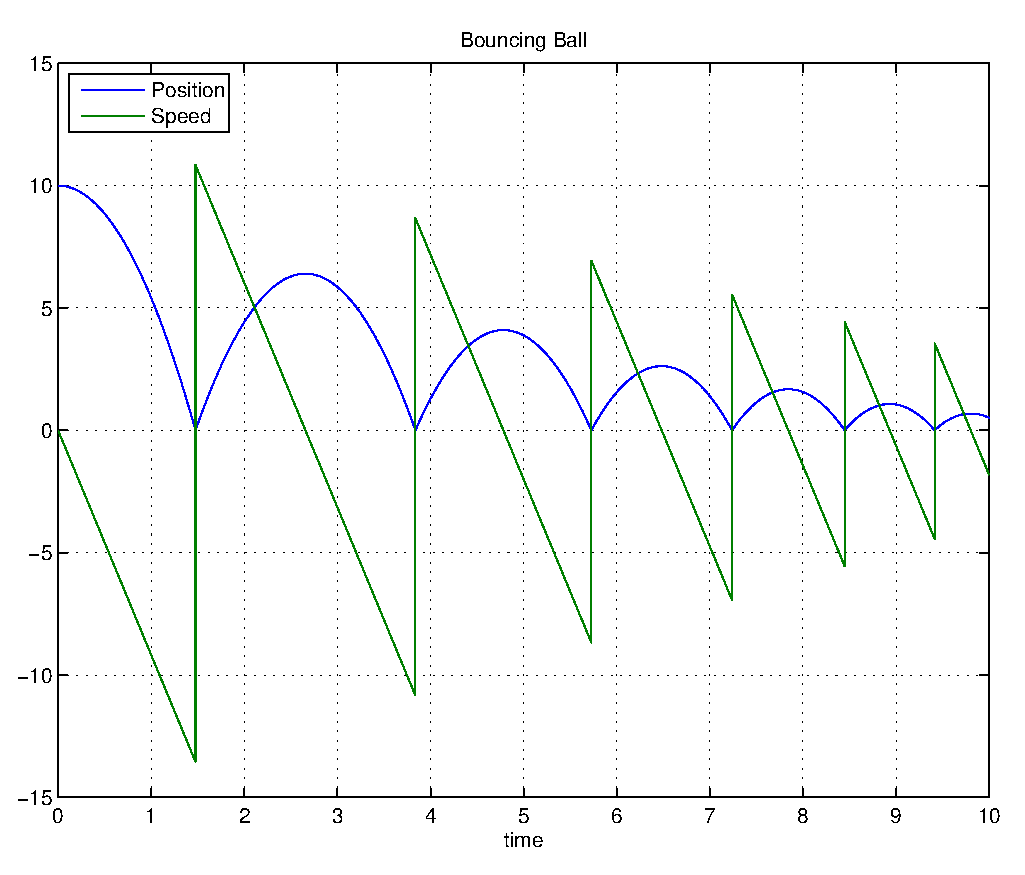
\includegraphics[width=0.45\textwidth]{bouncing_ball}
	\label{fig:bb}
	}
	\subfigure[Phase Plane]
	{
	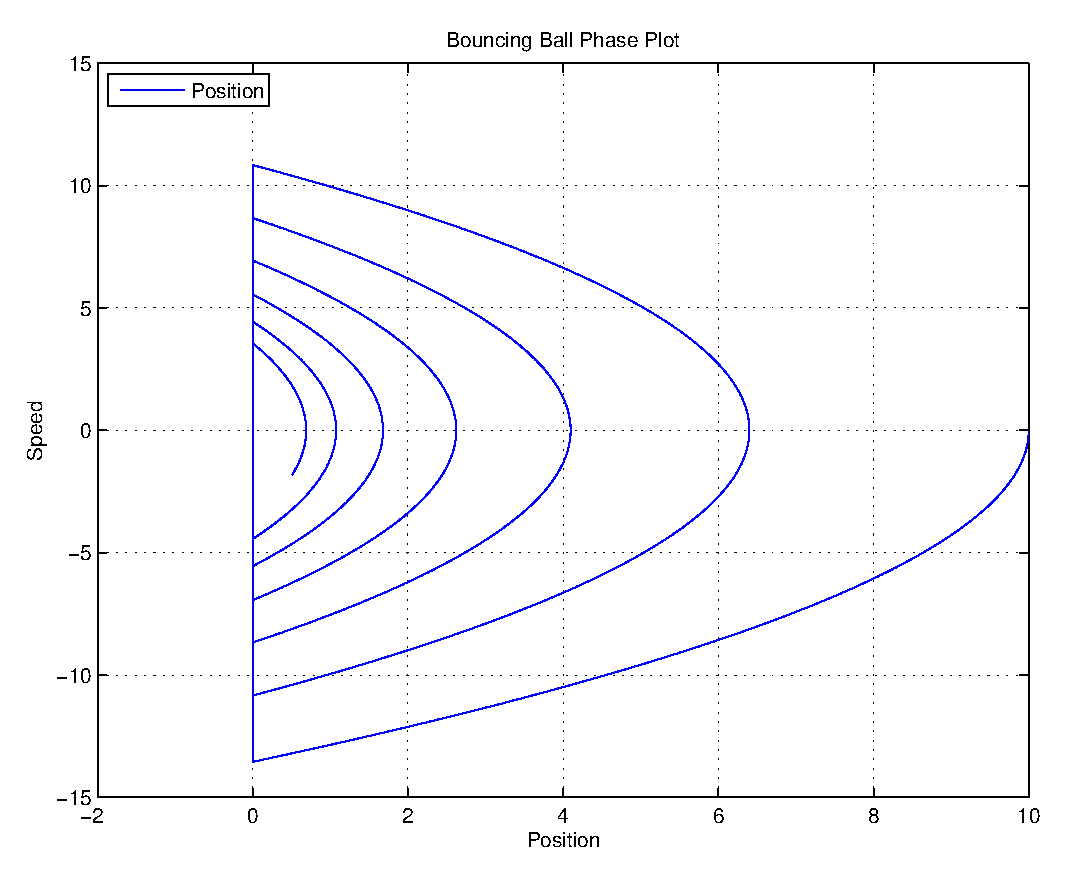
\includegraphics[width=0.45\textwidth]{bouncing_ball_phaseplot}
	\label{fig:bbp}
	}
	
\end{center}
\caption{Original Bourncing Ball System}
\label{fig:bborg}
\end{figure}



\subsection*{Emergence of Limit Cycle}
couple with neural oscillator boucing we get an limit circle
The input of neural oscillator is the velocity $\uin=\dot{q}_{ball}$, the output of neural oscillator  drive the pedal position $q_{pedal}=\uout$.
An limit circle emerge as the result of entrainment.
As show in figure drop from different position, all the ball will bouncing a about the same height of 5,as show in Figure~\ref{fig:bb_attractive_circle}

\begin{figure}[h]
\begin{center}
	\subfigure[state plot]
	{
	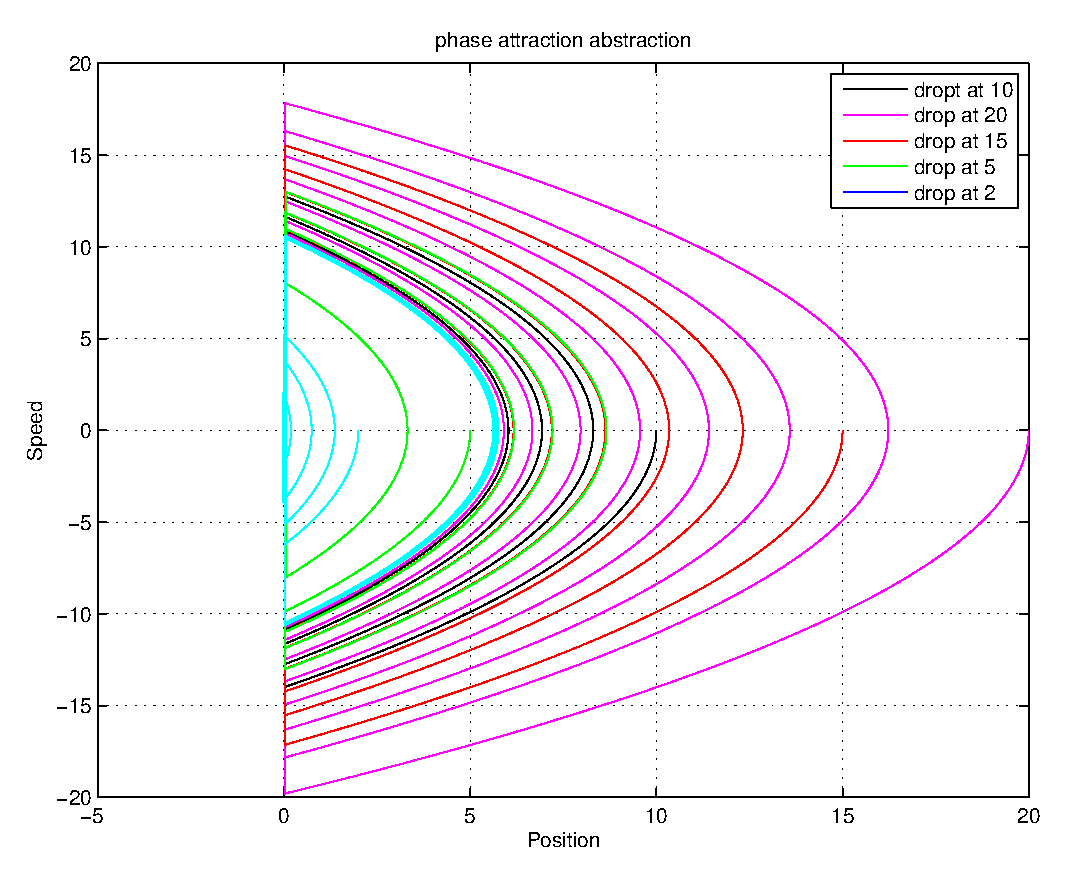
\includegraphics[width=0.45\textwidth]{bb_ms_os_attraction_phase}
	\label{fig:bb_attractive_entraint}
	}
	\subfigure[Phase Plane]
	{
	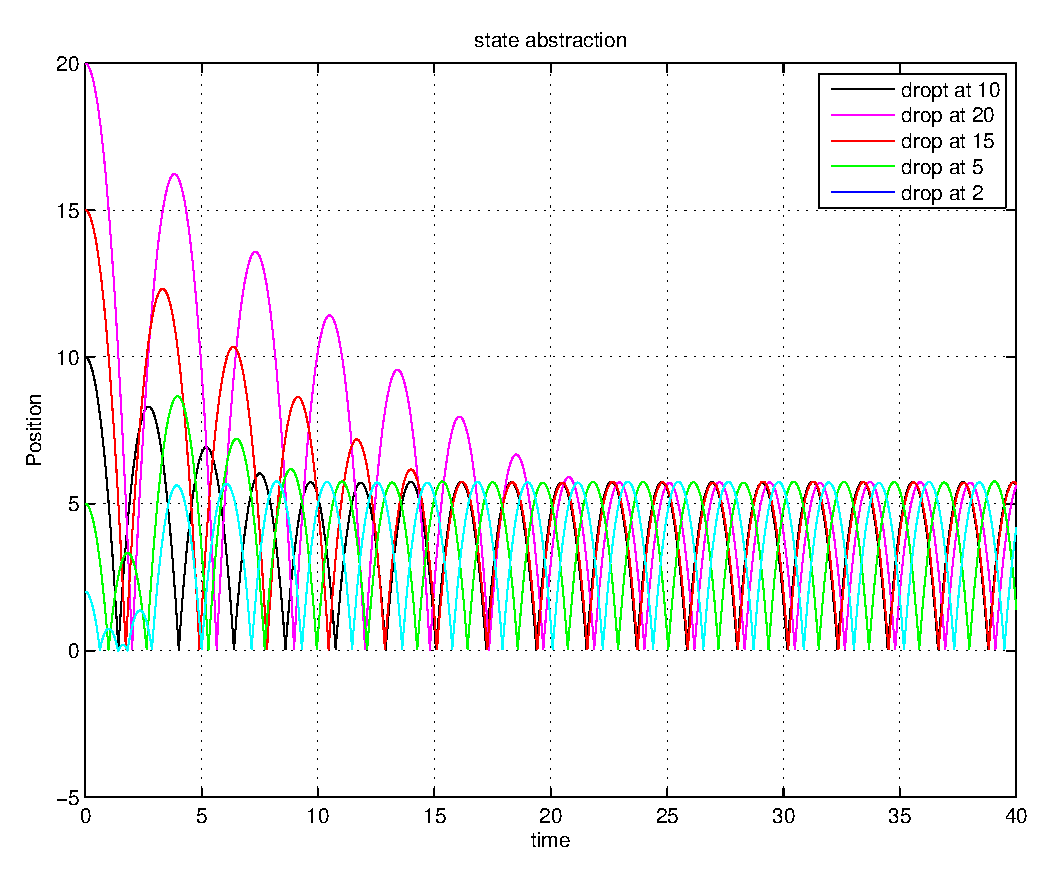
\includegraphics[width=0.45\textwidth]{bb_ms_os_StateTimeAttraction}
	\label{fig:bb_attractive_entraint_time}
	}
	
\end{center}
\caption{Attractive Limited Circle}
\label{fig:bb_attractive_circle}
\end{figure}

\chapter{LOCAL MOTOR INVARIANT}
\label{chap:li}

\nomenclature{$G$}{A Lie Group}
\nomenclature{$g_a$}{an elemetn in Lie Group $G$ with parameter $a$}
\nomenclature{$I(x)$}{Invariant Function of $x$}
\ifpdf
    \graphicspath{{LocalInvariant/LocalInvariantFigs/PNG/}{LocalInvariant/LocalInvariantFigs/PDF/}{LocalInvariant/LocalInvariantFigs/}}
\else
    \graphicspath{{LocalInvariant/LocalInvariantFigs/EPS/}{LocalInvariant/LocalInvariantFigs/}}
\fi

\section{Introduction}
Global Motor Invariant Control keeps the qualitative properties of motion primitives.
For animal motion is also of high accuracy.
In this chapter we focus on the control on the quantitative properties of motion.
In our research, we try to limit the computational cost.


The discovery is that motion of natural system will change in a uniform way.
The method we proposed exploring the symmetry properties of dynamics system.
The symmetry property of a dynamic system is called local motor invariant.
The method we propose is based the lie group theory.

\subsection{Group and Symmetry}
For the geometrical viewpoint, ''Symmetry''  means when you transform an shape, the transform one and original one are exactly the same.
For the square examples, rotation it by 90 degree will make it exactly the same with the original one.



\begin{figure}[!htbp]
  \begin{center}
    \leavevmode
    \ifpdf
      \includegraphics[height=6in]{Symmetry}
    \else
      \includegraphics[width=0.7\textwidth]{Symmetry}
    \fi
    \caption{Symmetry}
    \label{fig:symmetry}
\end{center}
\end{figure}


All the action that can preserve the symmetry is defined as the set as group $G$.
A group has the following properties.
\begin{itemize}
\item For any $g_a,g_b$ in $G$, \,$g_a*g_b$\, belongs to $G$. (The operation
``$*$'' is closed).

\item For any \,$g_a,g_b,g_c\in G$, \,$(g_a*g_b)*g_c=g_a*(g_b*g_c)$. \,(Associativity of
the operation).

\item There is an element $e\in G$ such that \,$g_a*e=e*g_a=g_a$\, for any
\,$g_a\in G$. (Existence of identity element).

\item For any \,$g_a\in G$\, there exists an element $g_h$ such that
\,$g_a*g_h=g_h*g_a=e$. \,(Existence of inverses).
\end{itemize}



In algebra sense, ''Symmetry'' means invariant, a shape can implicitly defined by an function $I(x)=0$;
The group transformation is define by $\hat{x}=g_a(x)$
If symmetry is met, we have $I(x)=I(\hat{x})$.
We can say $I(x)$ is an invariant function of group $G$.

We have to note that not only the one shape unchanged by $G$.
In fact ,many shape is invariant, 
In fact, we can pick up and two shape and combination is also an invariant shape. 
and form a space, the invariant space.


\begin{figure}[!htbp]
  \begin{center}
    \leavevmode
    \ifpdf
      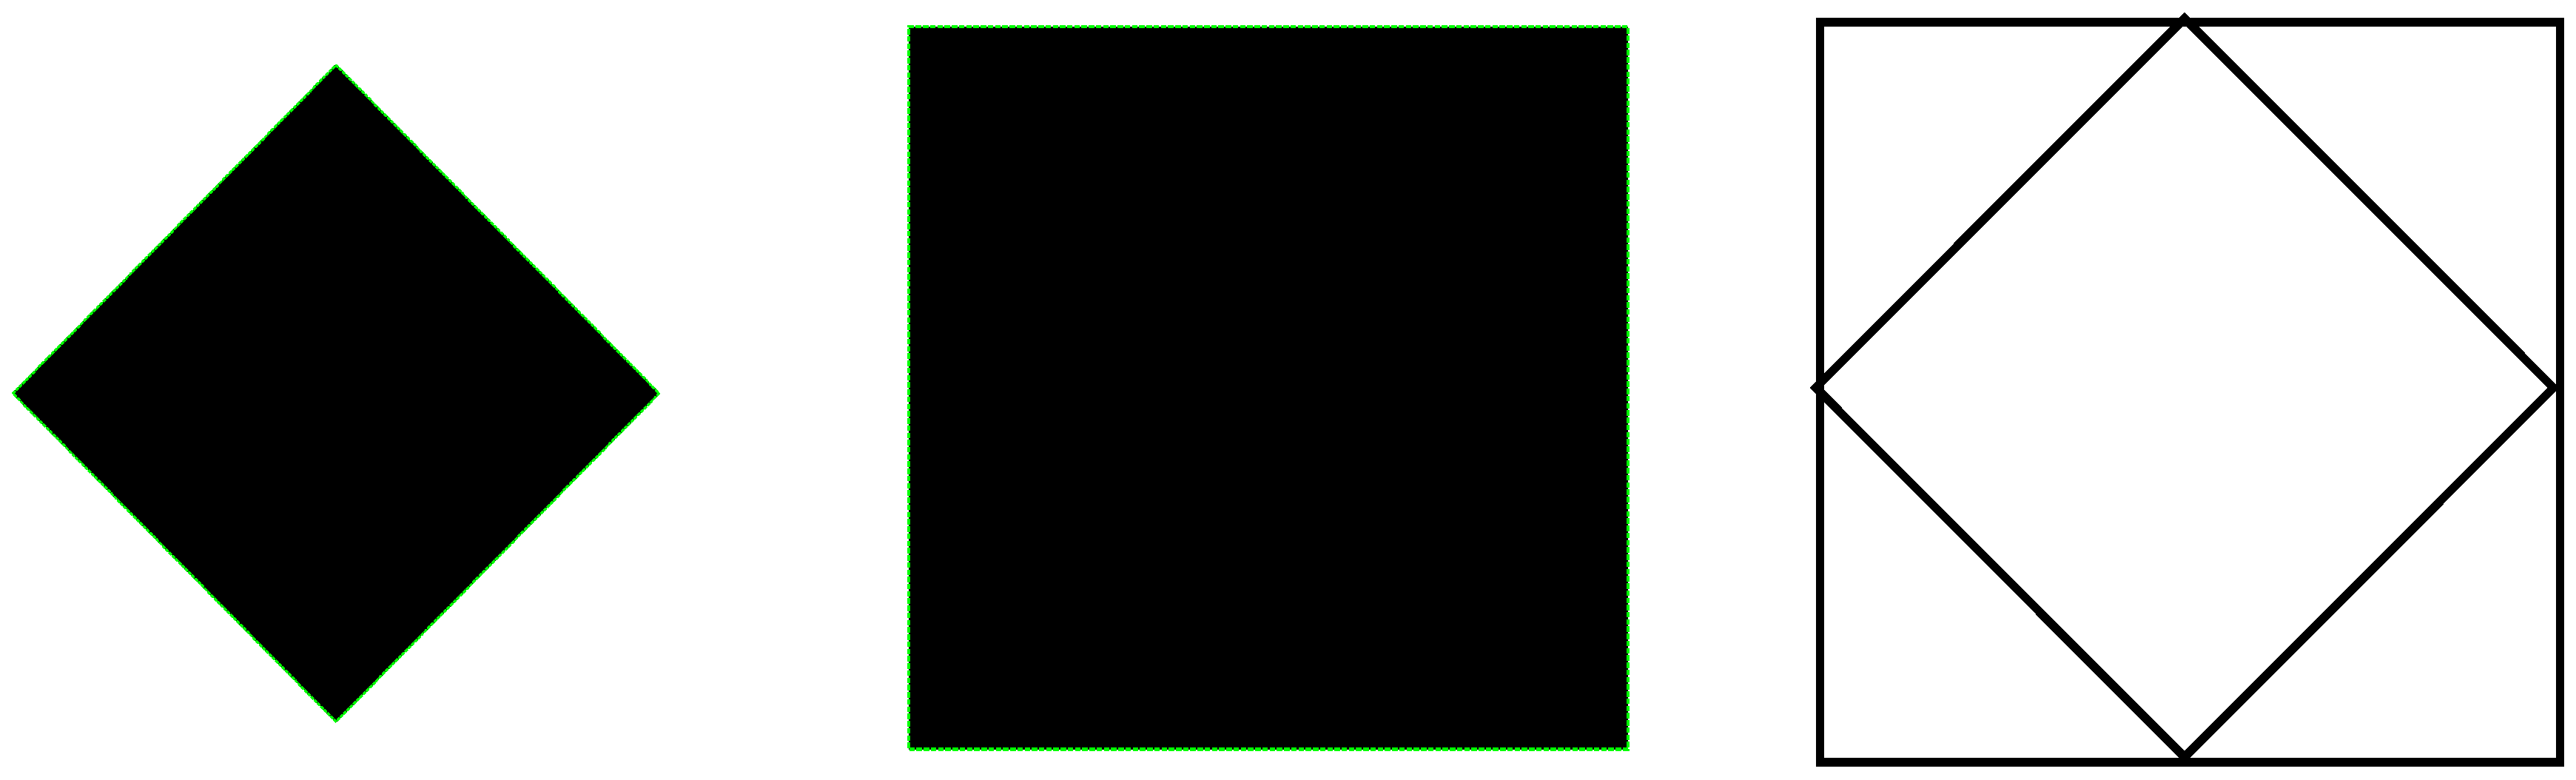
\includegraphics[height=6in]{SymmetrySpace}
    \else
      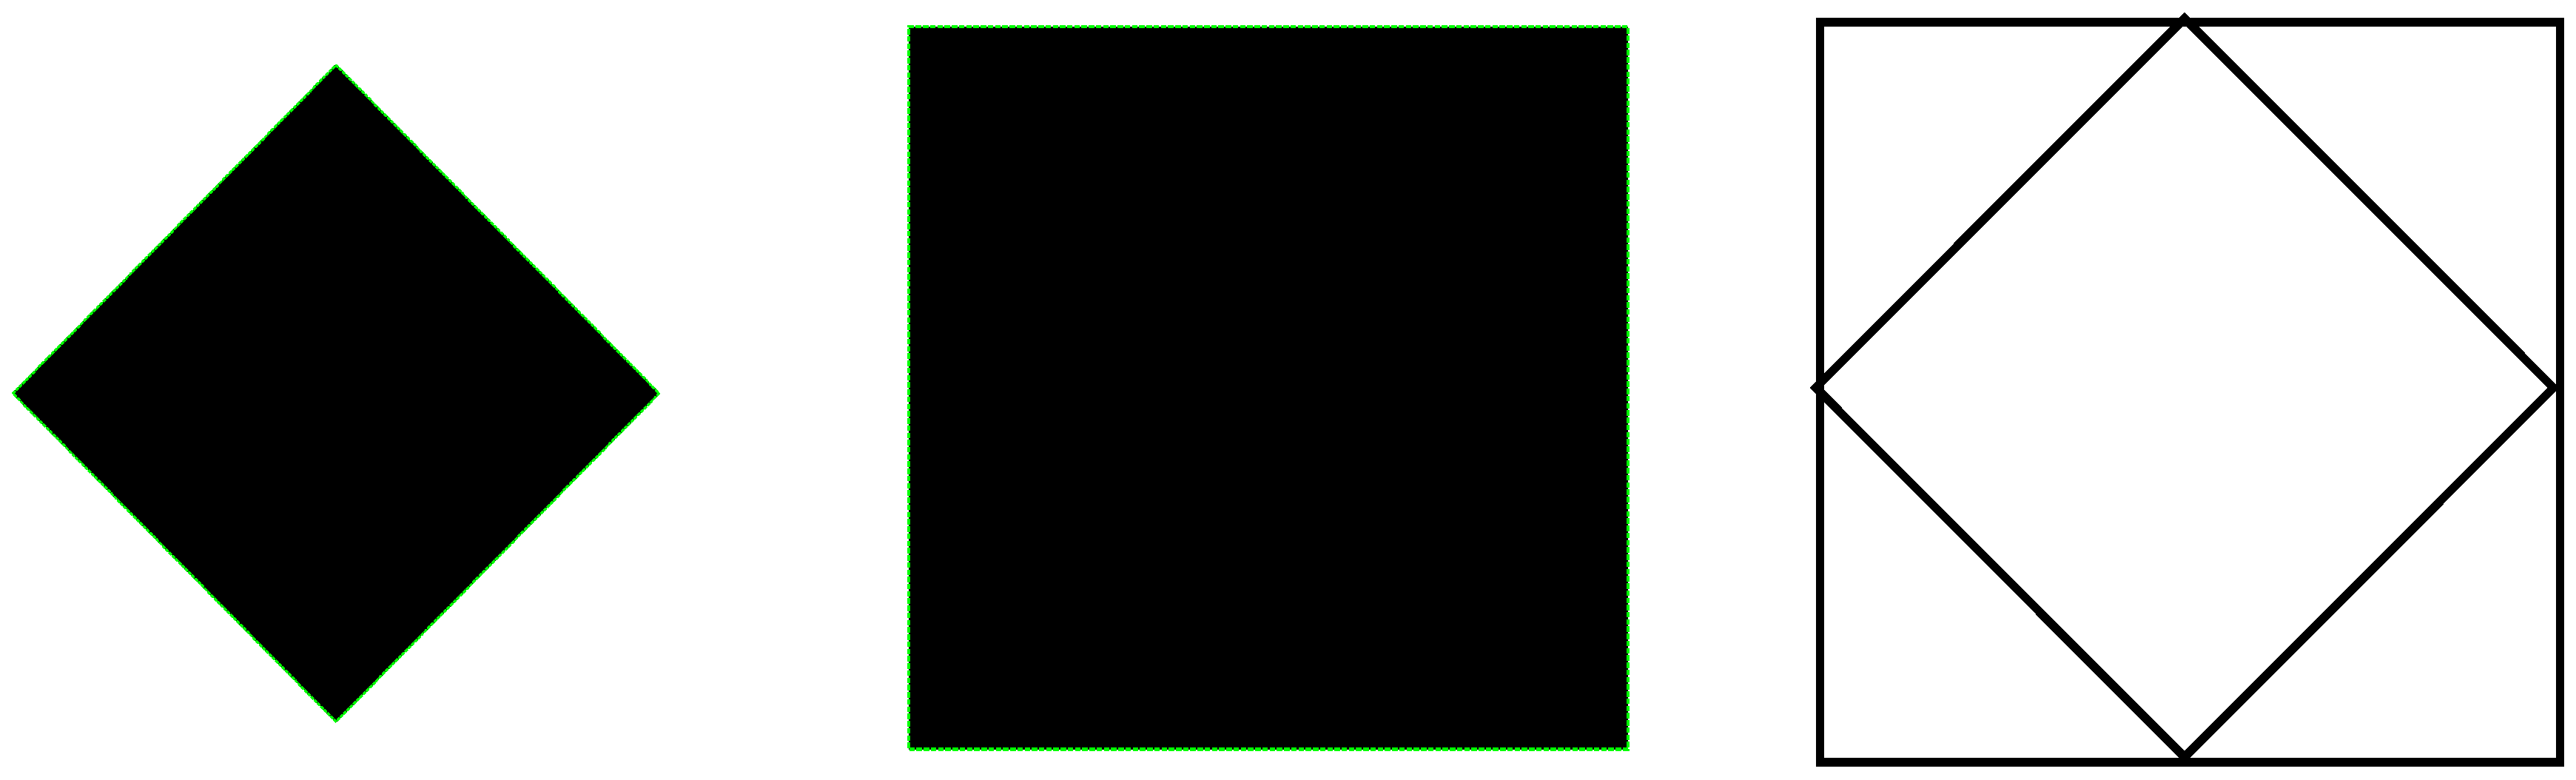
\includegraphics[width=0.7\textwidth]{SymmetrySpace}
    \fi
    \caption{Symmetry Space}
    \label{fig:symmetry Space}
\end{center}
\end{figure}





\subsection{Lie Group and Symmetry of Dynamic System}
Lie Group is continues group originates from study of differential equation.
For Physically-based animation,
Motion is usually described by the differential equation (1)
\begin{equation}
	\dot{\state}=F(\state)
\end{equation}
Lie Group $G$ will perserve the differential equation,for $g_a \in G$ 
\[
Tg_a(\dot{\hat{\state}})=F(g_a(\state)
\]
where $Tg_a$ is the corresponding lift action that transform the velocity $\dot{\state}$.
for example, if the $g_a$ is translate transformation, velocity will not be translate, then $Tg_a$ is identy.





Physically possible motion is the solution of the equation.
An important property from one solution $\state(t)$.
with a group action $g_a$, we can get another solution $g_a(x(t))$
 	
.
for example
, 
We have 

So the group action is


For equation (1), the group action $g_a$ satisfy the symmetry property (2).
	(3)
This provide us an idea about motion synthesis.
Given an original motion $q(t)$, and the corresponding group $G$, a new motion is generated by g(m).

For every group G, we can find an function I(x) unchanged by the group action G, 

I(x) are called local motion invariant. 
For mechanical system,  I(x) has important physically meaning. 
I(x) corresponding to the Conservative Law like energy or angular momentum.
\section{Controlled Symmetry}

For motion synthesis, usually the desired motion is ma
For example for motio stability, we want the current state is within the basin of attraction.
If we want to control the final motion style, we want the state is on the limit cycle.

For motion sysnthesis, the problem is given the system, let the original system have the desired symmetry.

 and original motion m is  known, but the corresponding group action $g_a$ is not satisfied by differential equation.
For such situation, control input u  is added, which modify the original equation to allow the designed G, this is called Controlled Symmetry.

Most dynamic motion can be modelled as an Lagrange System. 
\[
L=K(\dot(q)-V(q).
\]
And the desired action G must keep the L invariant. 

The original m is defined by the eural langrage equation
\begin{equation}
\frac{d}{dt} \frac{\partial L}{\partial \qd} - \frac{\partial L}{\partial q} = 0
\label{eq:uncontrolled_euler_lagrange}
\end{equation}
The modified system is 
\begin{align}
\frac{d}{dt} \frac{\partial L}{\partial Tg(\qd)} - \frac{\partial L}{\partial g(q)}&=0,\label{eq:liegroup_euler_lagrange}\\
\frac{d}{dt} \frac{\partial L}{\partial \qd} - \frac{\partial L}{\partial q}&=\ulocal. \label{eq:controlled_euler_lagrange}
\end{align}


(5) and (6) are the equivalent equation, by comparing  equation (5) and (6), we can get u
Some Specific example of Symmetry and Control
\subsection*{ Offset Action}
\[
\goff(q) = q+r
\]
Which keep speed, but modify the pos. thus keep the K but modify V

\begin{equation}
\ulocal(\x) = \frac{\partial}{\partial q} \left(V(\goff(q)) - V(q)\right).
\end{equation}

\begin{figure}[!htbp]
  \begin{center}
    \leavevmode
    \ifpdf
      \includegraphics[height=6in]{g_off}
    \else
      \includegraphics[width=0.7\textwidth]{g_off}
    \fi
    \caption{Offset Action}
    \label{fig:goff}
\end{center}
\end{figure}
on phase space, if q is the horizontal axis, and $\dot{q}$ is the vertical axis, this has the effect of moving the phase plot right and right.
\subsection*{Time Scalling}

%g_st(q,dot{q})=(q,st*dot{q})
we have
$T\gts(\qd)=\alpha \qd$
\begin{equation}
\ulocal(\x) = (\alpha^2 - 1) \frac{\partial V(q)}{\partial q}.
\end{equation}

\begin{figure}[!htbp]
  \begin{center}
    \leavevmode
    \ifpdf
      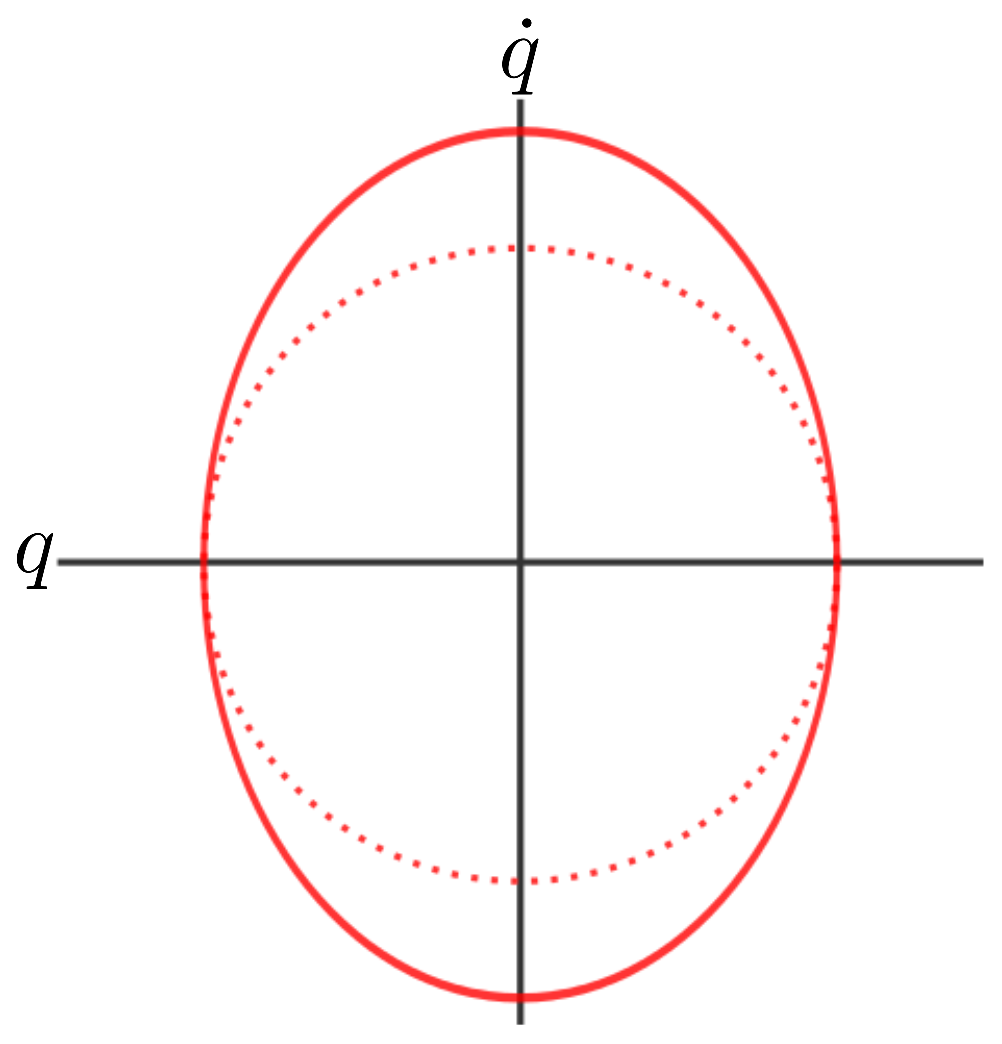
\includegraphics[height=6in]{g_ts}
    \else
      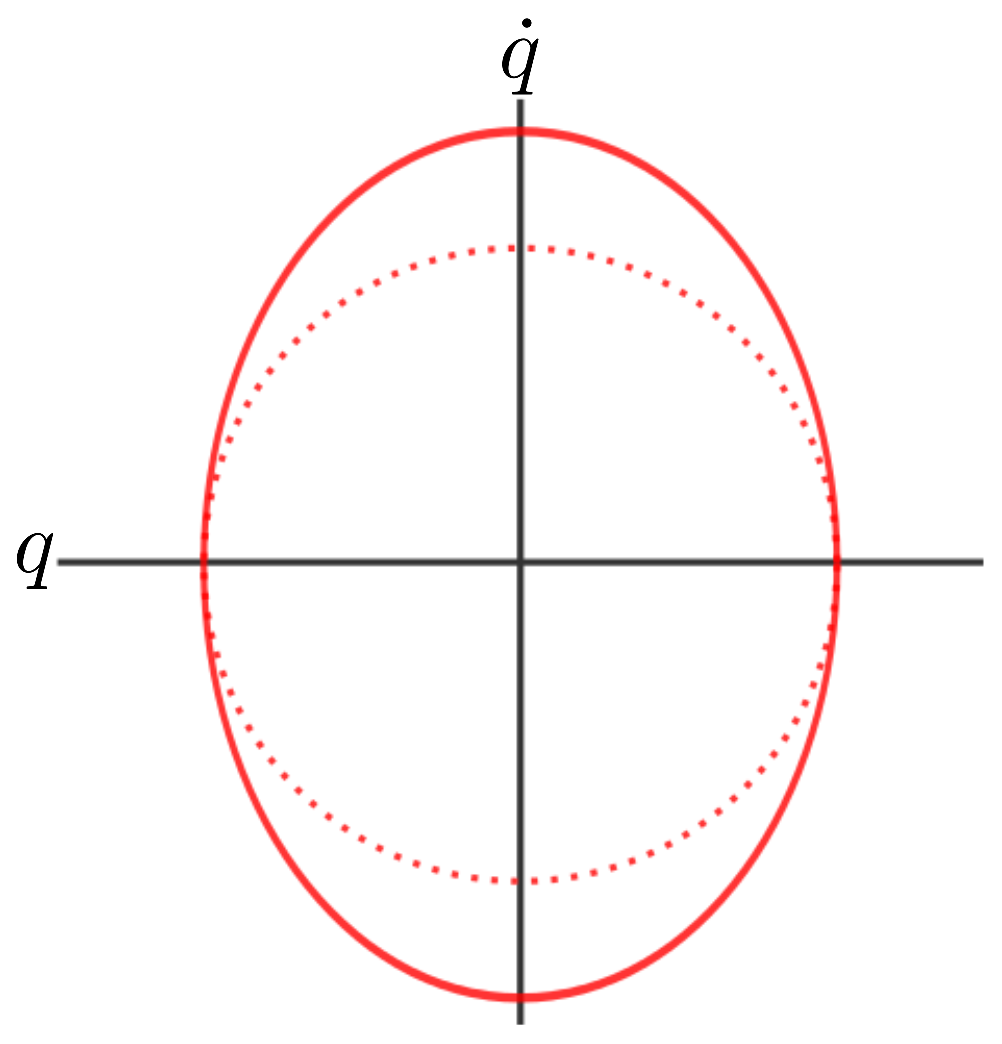
\includegraphics[width=0.7\textwidth]{g_ts}
    \fi
    \caption{Time Scaling Action}
    \label{fig:gts}
\end{center}
\end{figure}
on phase space, this has the effect strength the phase plot in the vertical direction

\subsection*{energy scaling}
For some system moving the the conservtime field with constant mass matrix.
The energy is preserved and different motion present different level of energy.
For such system, we have the 
For such

%g_e(q,\dot{q})=(e^2*q,e*\dot{q}).
U can be developed by applying the pos scaling and time scaling in a combined manner.

On phase plot, this has the effect enlarge the phase portrait.

\begin{figure}[!htbp]
  \begin{center}
    \leavevmode
    \ifpdf
      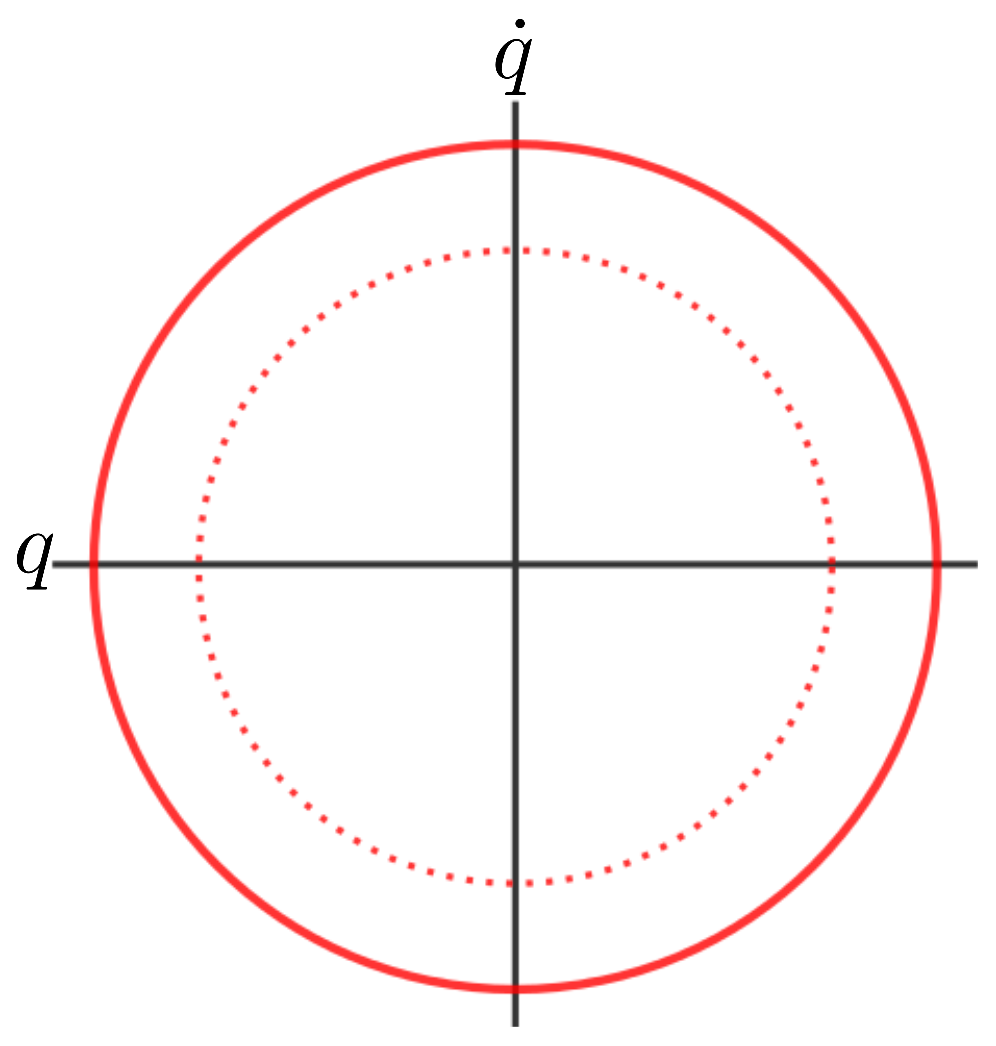
\includegraphics[height=6in]{g_en}
    \else
      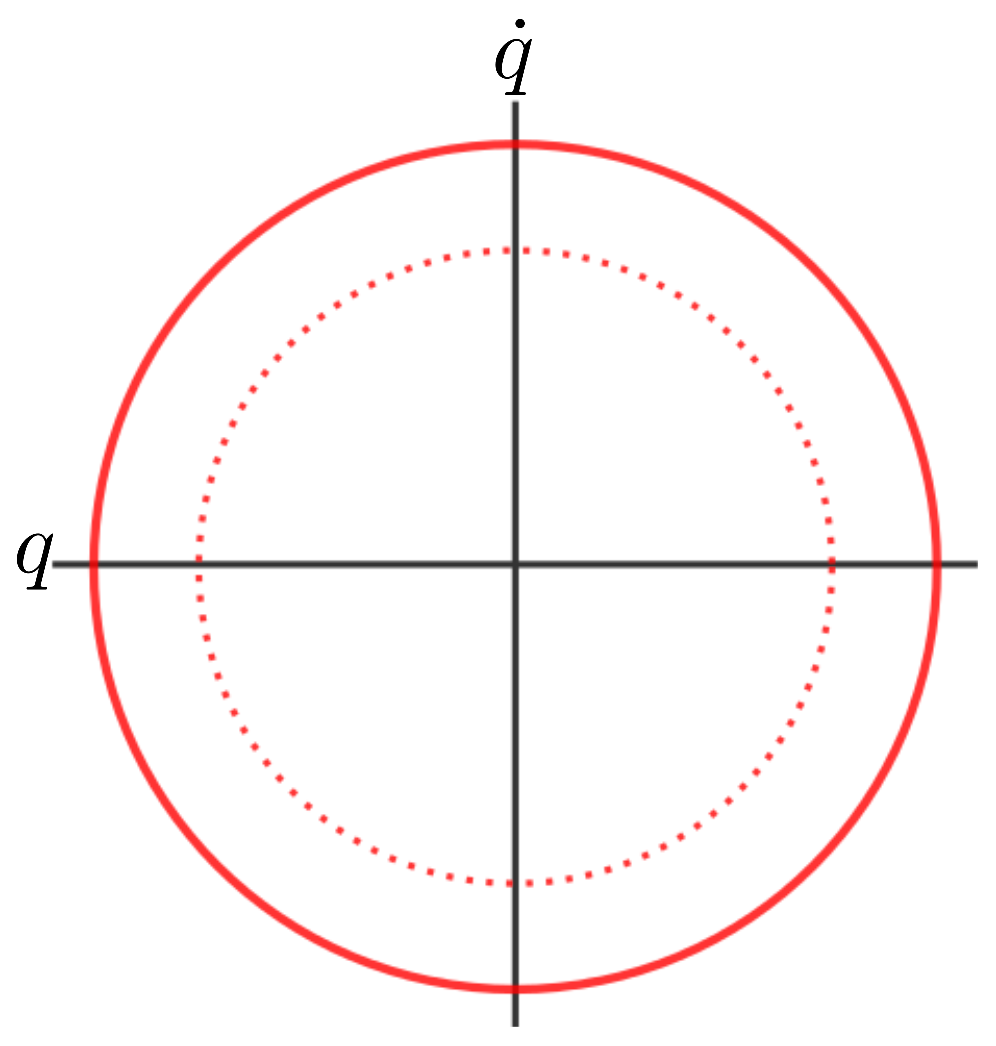
\includegraphics[width=0.7\textwidth]{g_en}
    \fi
    \caption{Energe Scaling Action}
    \label{fig:gen}
\end{center}
\end{figure}
\subsection*{time offset}
Is q(t) is solution to f(q)

%g_{toff}(q(t) \dot{q}(t))=(q(t+toff),\dot{q}(t+toff))
For dynamic system, this seems obvious. And no control is need for such symmetry.
For system with limit circle, this $g_toff$ has a special effects like phase modification.

On phase plot, this has the effect rotate on the limit circle about an angle.


\begin{figure}[!htbp]
  \begin{center}
    \leavevmode
    \ifpdf
      \includegraphics[height=6in]{g_off}
    \else
      \includegraphics[width=0.7\textwidth]{g_off}
    \fi
    \caption{Offset Action}
    \label{fig:goff}
\end{center}
\end{figure}





\section{Simple Example}
Bouncing Ball
The bouncing ball system has a energy scaling symmetry, if bouncing height is q(t), $\dot{q(t)}$
The new system is 
%Eq(t) \dot{e^2q{t}}

as show in figure

\begin{figure}[!htbp]
  \begin{center}
    \leavevmode
    \ifpdf
      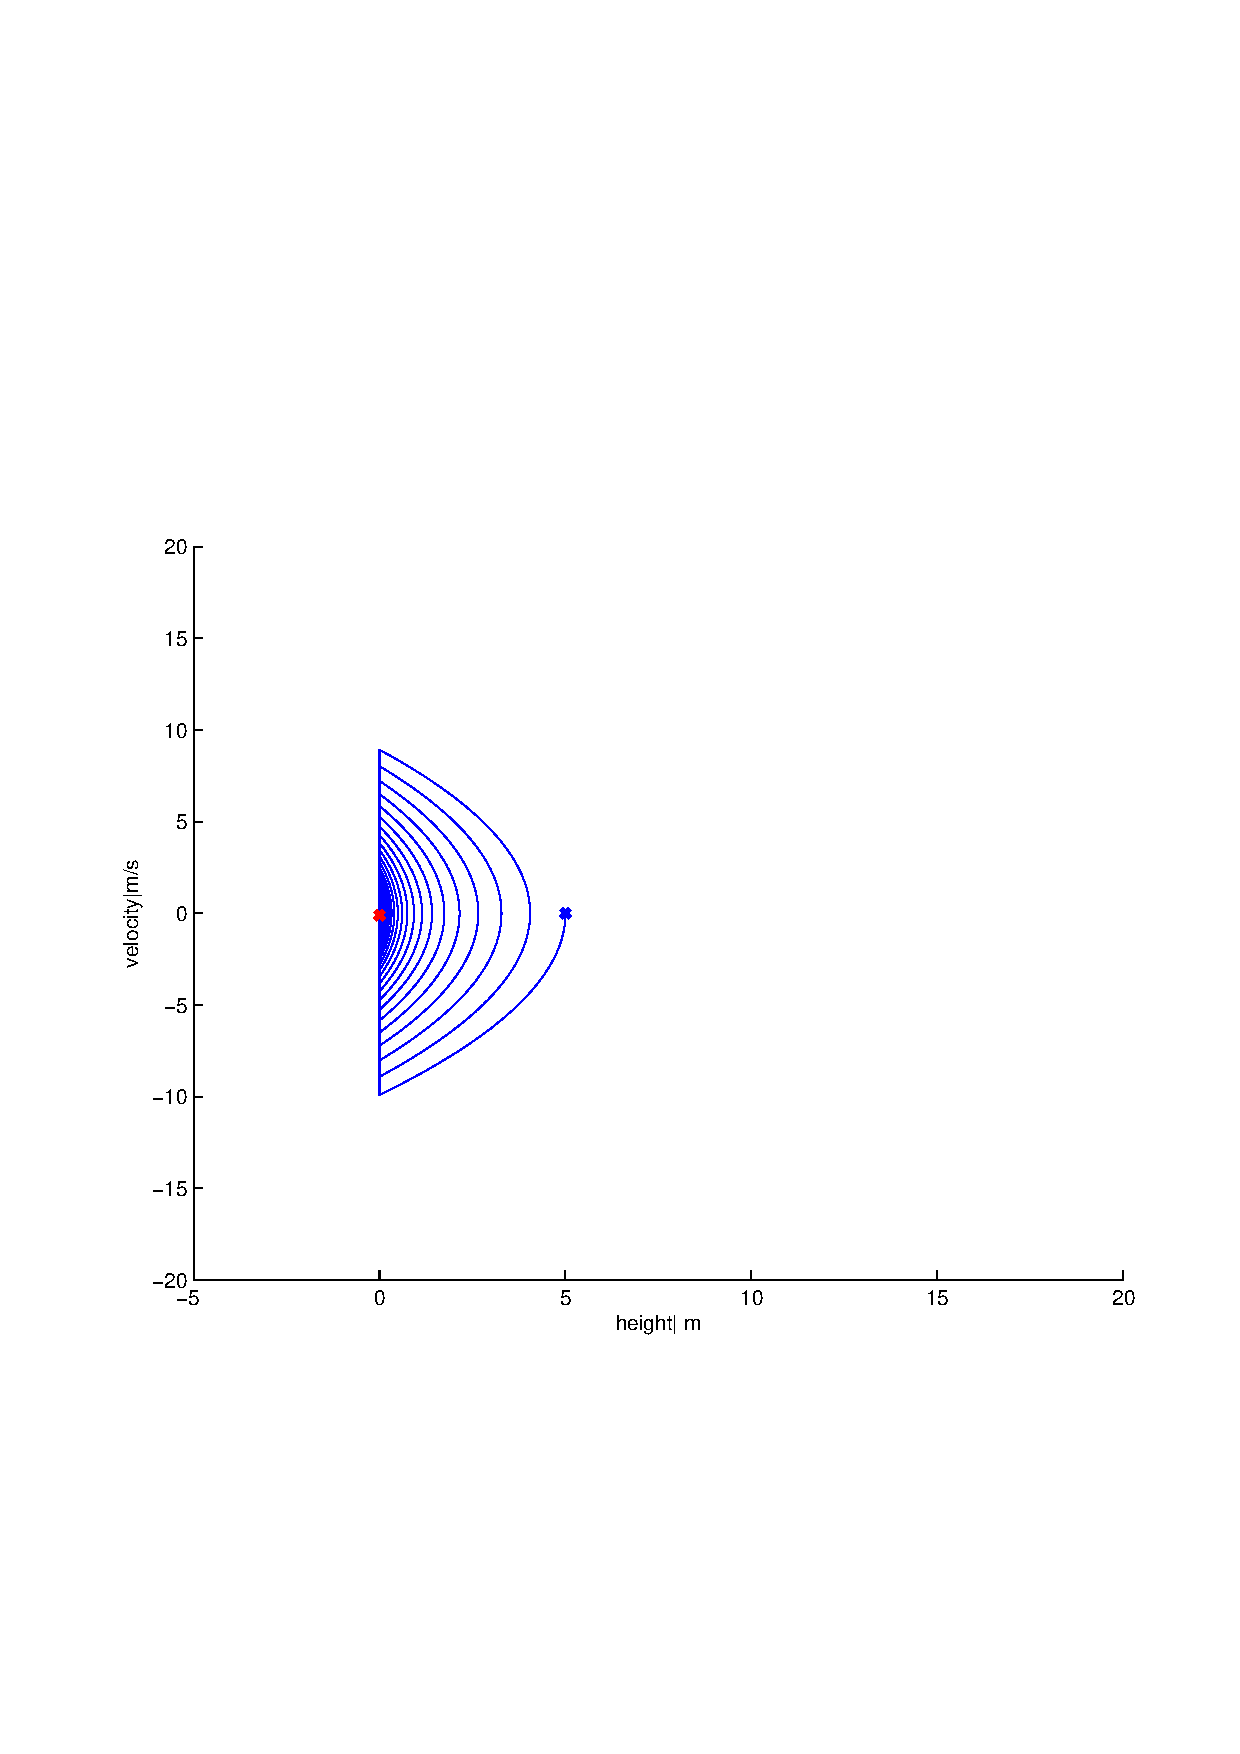
\includegraphics[height=6in]{BouncingBallPhasePlotuncontrolledDropAt5}
    \else
      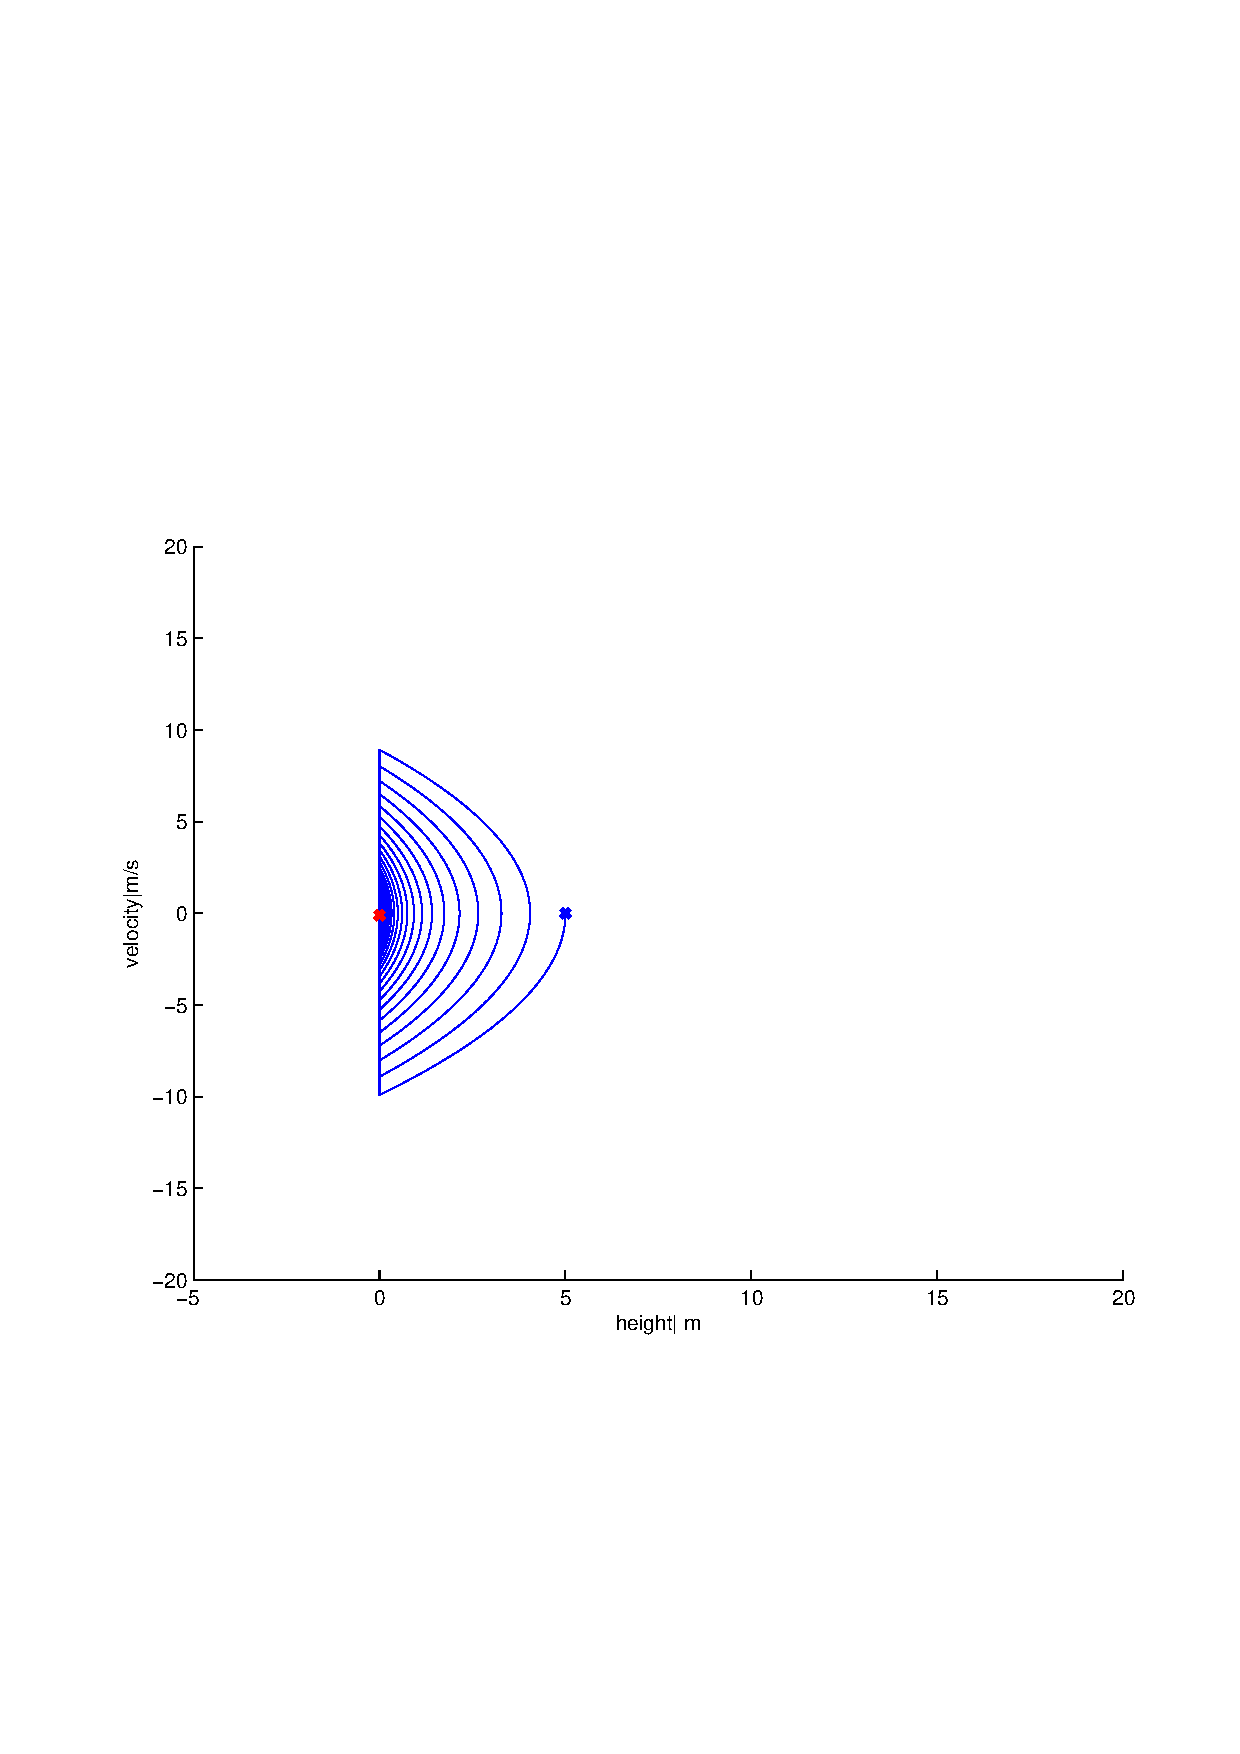
\includegraphics[width=0.7\textwidth]{BouncingBallPhasePlotuncontrolledDropAt5}
    \fi
    \caption{Drop at Filen}
    \label{fig:bouncing5}
\end{center}
\end{figure}


\begin{figure}[!htbp]
  \begin{center}
    \leavevmode
    \ifpdf
      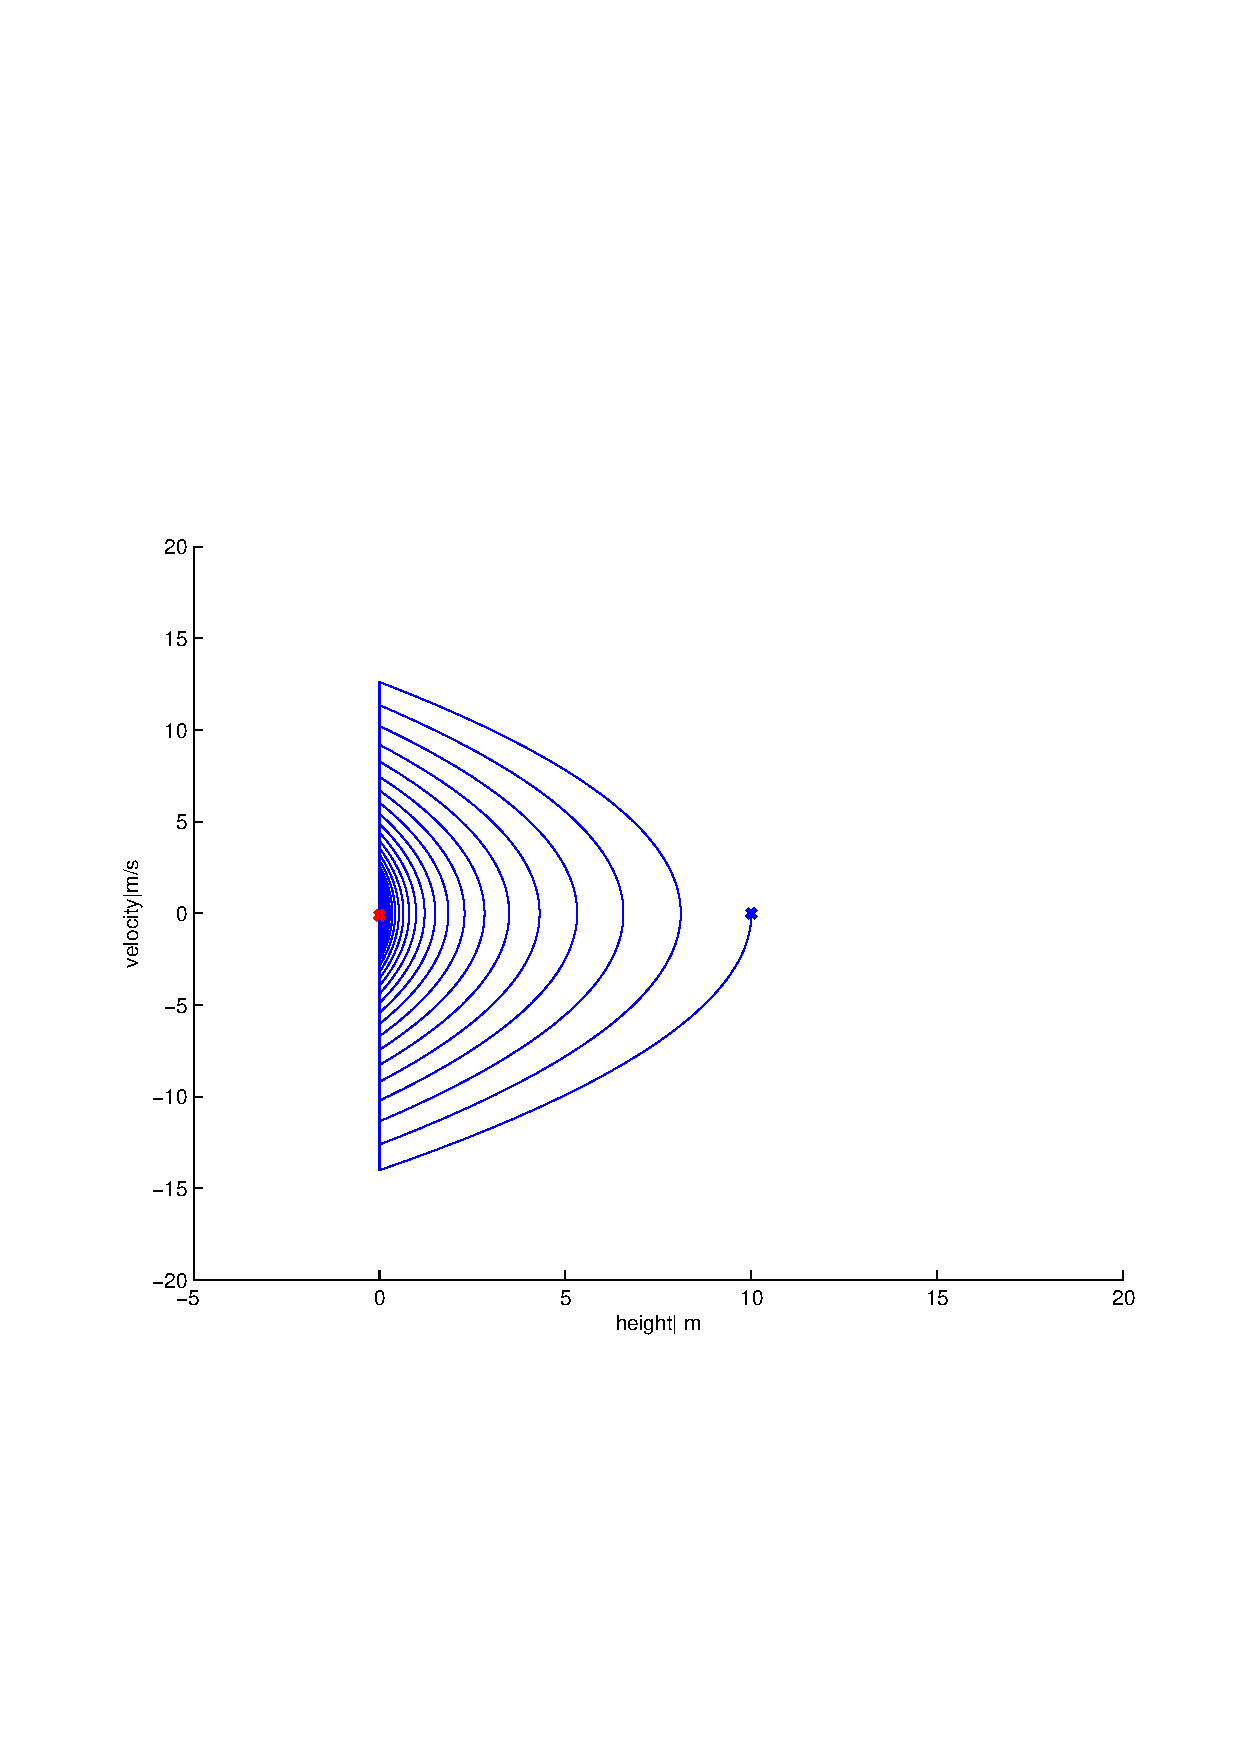
\includegraphics[height=6in]{BouncingBallPhasePlotuncontrolledDropAt10}
    \else
      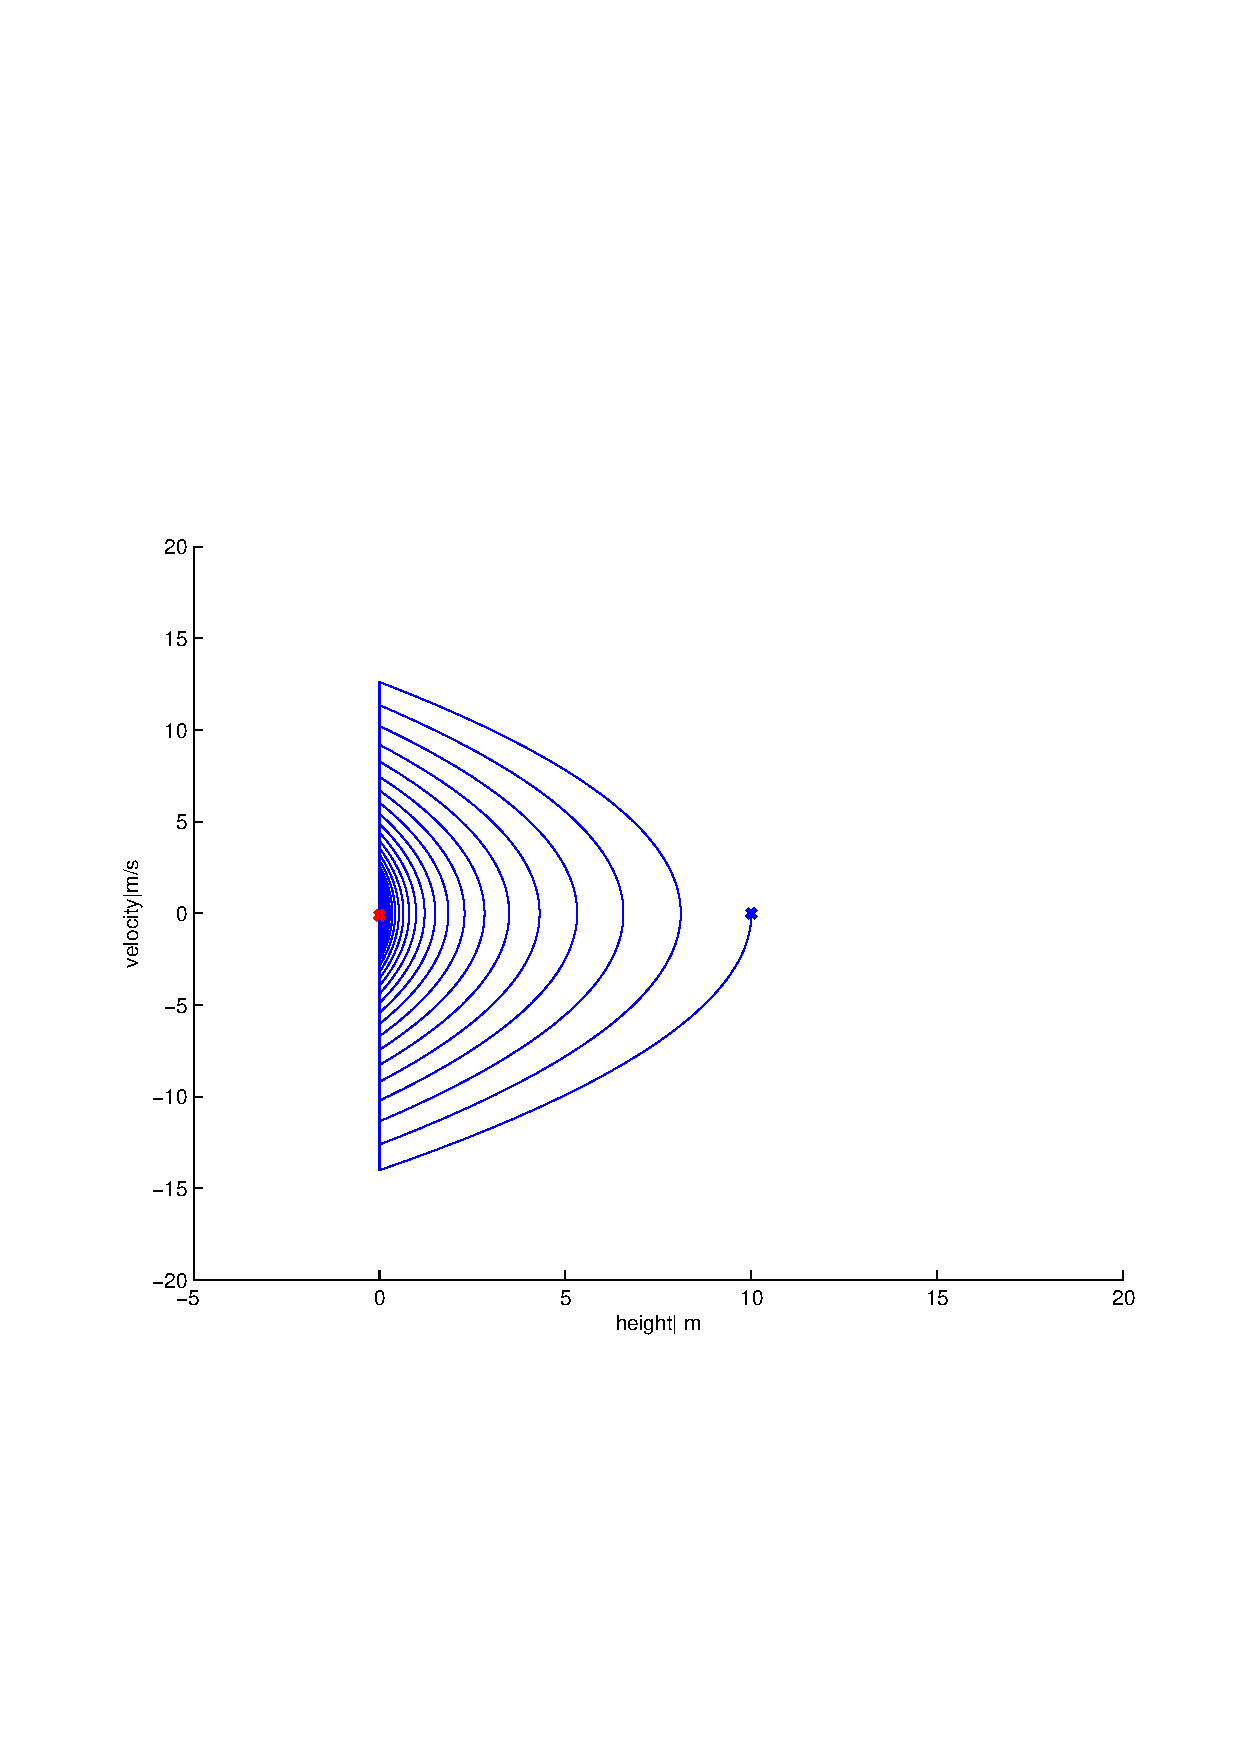
\includegraphics[width=0.7\textwidth]{BouncingBallPhasePlotuncontrolledDropAt10}
    \fi
    \caption{Drop at 10}
    \label{fig:bouncing5}
\end{center}
\end{figure}

\chapter {MOTION SYNTHESIS FRAMEWORK}
\label{chap:msf}
\ifpdf
    \graphicspath{{CombineFramework/CombineFrameworkFigs/PNG/}{CombineFramework/CombineFrameworkFigs/PDF/}{CombineFramework/CombineFrameworkFigs/}}
\else
    \graphicspath{{CombineFramework/CombineFrameworkFigs/EPS/}{CombineFramework/CombineFrameworkFigs/}}
\fi

Chapter 3 and Chapter Discussion some important idea of natural motion control properties from the mechanical viewpoint.
In this chapter ,we will dicuss how we combine the idea from Chapter 3 and Chapter 5 into meaning full motion synthesis System.
Mainly we will discuss two question,
\begin{itemize}
\item how global and local motor invariant controller work together.
\item how combine different motion primitives together.
\end{itemize}

\section{Combined Global and Local Motor Invariant}

\subsection{ motor control idea based on Global and Local  Motor Invariant.}

Neural Oscillator will maintain the qualitative motion properties, and Controller Symmetry will satisfy the quantitative properties.
Basically we need apply the qualitative controller first to maintain the topology against the structural perturbation, 
when Symmetry Controller is applied to transform the entrainment System to meet some specific user constraints.


Snimply put, we should get the qualitative write first, and then get the quantitative write .
This idea is straightforward is illustrated in the following example
\begin{figure}[!htbp]
  \begin{center}
    \leavevmode
    \ifpdf
      \includegraphics[height=6in]{LimitCircle}
    \else
      \includegraphics[width=0.7\textwidth]{LimitCircle}
    \fi
    \caption{System Over View }
    \label{fig:sysoverview}
  \end{center}
\end{figure}
but when applying this method, we have condition must be met.
\begin{itemize}
\item unlike the CPG controlled example discussed in Chapter 3, when must maintain the topology when the symmetry controlled is applied.
To met this condition, we must prove that Symmetry Controller will not violate the topology, and symmetry control is applied to the how system rather than the original system.

We must prove that Lie Group Operator will not violate the topology

\item In chapter 4 we discuss the controlled symmetry is applied to the original system, how ever, for motion synthesis, we must prove that the combined system should preserve the symmetry.

If the original system $F(x)$ have the symmetry property, we also require the neural oscillator have the same symmetry properties.
Thus we need to discuss how to transform the Neural Oscillator so the neural oscillator have the same kind of symmetry as the mechanical oscillator
\end{itemize}



\subsection{ Controlled Symmetry Preserved The Topology}

Theorem Controlled Symmetry is Topology Preserving
suppose the original system is $\dot{x}=F(x)$, Controlled system is $\dot{G(x)}=F(G(x))$,
proof :
	by the demotion mation, G is continues and one one mapping.
	The the the original system and transformed system are isotropy.
	Thus Controlled Symmetry is topology Preserving


\subsection{ Symmetry of Neural Oscillator.}
We separate the discussion

after coupling with neural oscillator, the $\dot{x}=F(x)$ becomes a system 
$\dot{x}=F(x)+u_in$
for controlled system, when must maintain
$\dot{G(x)}=F(G(x)+u_ing$

for the neural system
the the dynamic equation is

$\dot{xc}=S(x_c)+uin$
we requires te symmetry must meet
$\dot{G(xc)}=S(G(x_c)+u_ing$
the out put function is
$O(x_c)$


for the symmetry property, we must statisfy the following following follow equation
$u_inG=O(x_cG)$
$u_inG=O(xg)$

For must our research, we find that we only adjust the three parameters of the neural oscillator to meet equation above
$\tau,hi,ho$
and some examples are included.

\subsubsection*{ offset Symmetry.}
For offset symmetry, we carefully select the $U_in$ and $U_out$ acting on the Invariant variables.
For example ,when walking slope changes, we choose the input of the neural oscillator to be the angle between the joints or velocity difference,
then all the input function will not change, if the output of the neural oscillator is apply not directly the q, but to the difference of q of velocity of q,
then the out put function can is also unchanged.


\subsubsection*{Time Scaling}
Neural Oscillator can change its Speed by changing ts.
We prove change ts, we can maintain the same is maintained.

For the dynamic system, usually control will affect the second order derivative.
Then we can u needs to be $ts^2$ the original system.
So we can multiply $hout=ts^2$ hout

\subsubsection*{ Energy Scaling}
energy scaling is $G(x)=(G(q),G(\dot{q})$
$q=sq$,
$\dot{q}=t(s)q$

it is equal to apply the scaling of the configure q and time scaling sequentially.
For our research, we apply the speed action to the neural oscillator first,
when scaling the h to keep the input keep constant.


\subsubsection*{time offset }
Neural Oscillator don't have to do any thing with the state,
but it also have to rotate its state.


\subsection{A simple example}

Bouncing Ball

\begin{figure}[!htbp]
  \begin{center}
    \leavevmode
    \ifpdf
      \includegraphics[height=6in]{BouncingBallPhasePlotAction1}
    \else
      \includegraphics[width=0.7\textwidth]{BouncingBallPhasePlotAction1}
    \fi
    \caption{Energy Scalling}
    \label{fig:energy1}
  \end{center}
\end{figure} 


\begin{figure}[!htbp]
  \begin{center}
    \leavevmode
    \ifpdf
      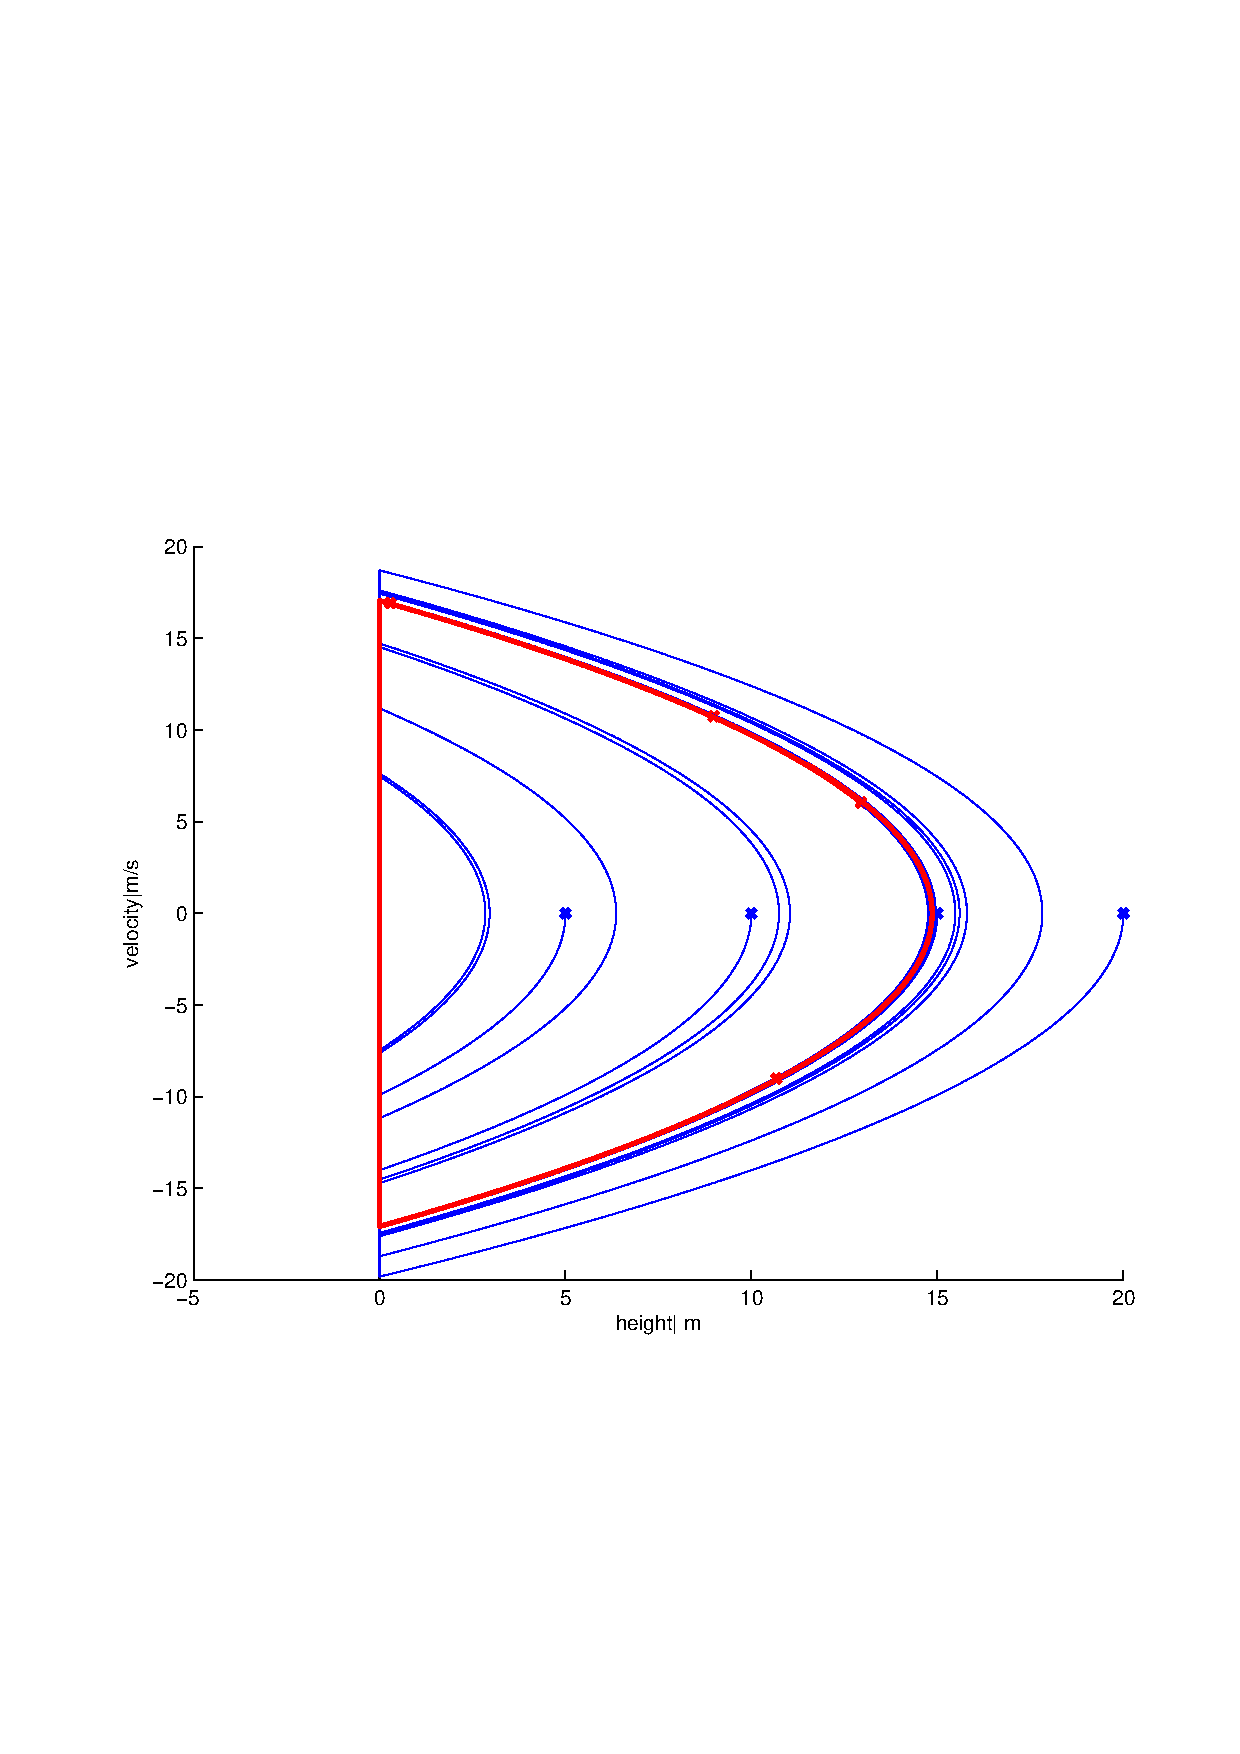
\includegraphics[height=6in]{BouncingBallPhasePlotAction3}
    \else
      \includegraphics[width=0.7\textwidth]{BouncingBallPhasePlotAction3}
    \fi
    \caption{Energy Scaling}
    \label{fig:energy3}
  \end{center}
\end{figure}

\section{Combine Motion Primitives}

\subsection{The Motion Primitives Graph}
Motion Primitives comes from the original mechanical system, motion primitives can only transformed if they are neighbours.
Following this idea, given a dynamic system we can draw a graph of motion primitives and this is called motion primitives graph.
The idea is very similar to the motion graph, the difference here is in the original motion graph are handed  crafted, 
while in our research, we propose that a motion graph of a dynamic system is fixed, at from any motion primitives, the way he can change its motion is also limited.

\begin{figure}[!htbp]
  \begin{center}
    \leavevmode
    \ifpdf
      \includegraphics[height=6in]{MotionPrimitiveGraph}
    \else
      \includegraphics[width=0.7\textwidth]{MotionPrimitiveGraph}
    \fi
    \caption{Phase Plot of Motion Primitives}
    \label{fig:manyprimitives}
  \end{center}
\end{figure}


\begin{figure}[!htbp]
  \begin{center}
    \leavevmode
    \ifpdf
      \includegraphics[height=6in]{motiongraphtopology}
    \else
      \includegraphics[width=0.7\textwidth]{motiongraphtopology}
    \fi
    \caption{Phase Plot of Motion Primitives}
    \label{fig:manyprimitives}
  \end{center}
\end{figure}


\subsection{The Motion Primitives Transition}

From dynamic point of view, changing motion primitives is put the current state in the basin of attraction  of one attractor into the basic of attraction of another attractor.
As show in picture, for the uncontrolled system, the transition will not happen automatically, for the two basic of attraction will not overlap.

To put the state x in basin of attraction, have two methods.


\begin{figure}[!htbp]
  \begin{center}
    \leavevmode
    \ifpdf
      \includegraphics[height=6in]{MotionPrimitiveTransition}
    \else
      \includegraphics[width=0.7\textwidth]{MotionPrimitiveTransition}
    \fi
    \caption{Motion Primitive Transition}
    \label{fig:motion-transition}
  \end{center}
\end{figure}

\begin{itemize}
\HiItem{ Overlaping Method}
The first idea is use different CPG for different motion primitives. There is a switch mechanism of switching the CPG.
If cpa a is applied to the fx, then the basic off attraction is enlarged, if cpg b is applied to motion primitives b,
the basin of attraction is also enlarged.
If a system is at state that within the both basin of attraction, we can switch the CPG controller.

\begin{figure}[!htbp]
  \begin{center}
    \leavevmode
    \ifpdf
      \includegraphics[height=6in]{OverLayTransition}
    \else
      \includegraphics[width=0.7\textwidth]{OverLayTransition}
    \fi
    \caption{Over Lay Transition}
    \label{fig:motion-transition}
  \end{center}
\end{figure}


\HiItem{Transform Method}
Controlled Symmetr can also applied for motion state transition.
For a system at x , we can transform the phase portrait to make it which in the basic of attraction of b,
this is illustrate in figure 


\begin{figure}[!htbp]
  \begin{center}
    \leavevmode
    \ifpdf
      \includegraphics[height=6in]{OffsetTransition}
    \else
      \includegraphics[width=0.7\textwidth]{OffsetTransition}
    \fi
    \caption{Offset Transiton}
    \label{fig:transform-transit}
  \end{center}
\end{figure}
\end{itemize}




Both the method can result in physically realistic motion transition, when the current state x lies a a special position.
The what more problem happens when we don't know is where the current position x and where it is going.
Thus we combined the two method above to achieve for a combined method,
no matter where is current point is, it is going to converge to the limit cycle, thus we ask both basic of attraction cover the limit cycle, this can be achieved via using both the CPG and Transformation.
And for this usually ,both motion primitives needs to be transformed,
And the there is relationship between the two transformation,  this relation ship is called transformation connection.

Figure download show the illustrate the idea.

\begin{figure}[!htbp]
  \begin{center}
    \leavevmode
    \ifpdf
      \includegraphics[height=6in]{ConbineMethod}
    \else
      \includegraphics[width=0.7\textwidth]{ConbineMethod}
    \fi
    \caption{Comined Method}
    \label{fig:Combine}
  \end{center}
\end{figure}



\chapter{MOTION PRIMITIVE TWEAKING:BIPEDAL WALKING}
\label{chap:walk}
\graphicspath{{BipedWalk/BipedWalkFigs/EPS/}{BipedWalk/BipedWalkFigs/}}


The examples of bouncing ball and mass spring systems only illustrate the theory, but have little application value.
This chapter discusses in details about how to adapt a motion primitive for  environmental and application specific constraints.
Combination and transitions of motion primitives are discussed in the next chapter.


The motion primitive understudy in this chapter is \emph{bipedal walking}, which is a topic of great application value for both the graphic and robotic engineering.
In the past decades, many methods have been applied to the bipedal walking, but still we have not achieved  human bipedal walking ability yet.
The early belief is that bipedal walking in nature is unstable, and many control methods are developed based on trajectory following.
The turning point is the discovery of passive dynamic walking machine, which shows under specific conditions, walking needs not control effort.
This idea lead us to believe that walking is an inborn ability, and most problems are solved by the mechanical structure.

In motor invariant theory, bipedal walking is  a motion primitive.
The passive walking gait is treated as the template.
Neural Oscillator and Symmetry Control are applied to tweaking the template while maintaining the global and local motor invariants.
This method generate adaptive gaits and stable gaits in realtime.




\section{Motion Primitives}


For bipedal walking, yaw and roll motion are relative small and usually treated as secondary motion or totally neglected,  main motion happens in the \emph{sagittal plane}, as shown in Figure~\ref{fig:passivekneewalker}
as shown in figure
\begin{figure}[!htbp]
  \begin{center}
    \includegraphics[width=0.7\textwidth]{spahittalPlae}
    \caption{SpahittaPlane}
    \label{fig:passivekneewalker}
\end{center}
\end{figure}




This chapter focuses on the motions in sagittal plane,  \dof s in coronal plane are discussed in Chapter~\ref{chap:highdor}.
More \dof s will introduce perturbations to our model, but will not change the basic motion characteristics and adaptation tendency.
They will make the ``symmetry'' not so perfect and may cause confusions in explaining the idea. thus the discussion is delayed.


The passive walking machine is shown in Figure~\ref{fig:passivekneewalker}.

\begin{figure}[!htbp]
  \begin{center}
    \includegraphics[width=0.7\textwidth]{PWI}
    \caption{A Passive Walking Model with Knee}
    \label{fig:passivekneewalker}
  \end{center}
\end{figure}



\subsection*{Dynamics}

Like the bouncing ball system, this system is hybrid\citep{ames2006categorical}, includes continuous and discrete dynamics[].
Passive walking with knees include four phases\citep{Chen2007}.
\begin{itemize}
\HiItem{Free Swing Phase}
The support leg (the blue one) is kept straight,during this phase the knee of the swing leg is bended, the thigh and shank swings freely.
\HiItem{Knee Strike Phase}
The knee joint of the swing leg has a limit.When the knee angle reach the limit,a collision happens.
After the collision, the swing leg is kept straight.
\HiItem{Knee Lock Swing Phase}
During this swing phase, both the swing and support leg are kept straight.
\HiItem{Heel Strike Phase}
When the heel of the swing leg hits the ground, a collision happens and after that the swing and support legs are switched.
\end{itemize}


The passive walker is modelled based on rigid body dynamics.
Dyanmic equations are developed based on Lagrange Mechanics~\citep{Goldstein2002}.
for details of calculating the dynamic equation, please reference\citep{Chen2007}



\begin{itemize}
\HiItem{Flying Phases}
For both the free and locked knee swing phases are described by the continuous dynamics.
Both equations are in the form of Equation~\ref{eq:flyequation}.
\begin{equation}
\label{eq:flyequation}
M(\mathbf{q}) \ddot{\mathbf{q}} + C(\mathbf{q,\qd})\dot{\mathbf{q}} + N(\mathbf{q}) = 0
\end{equation}
$q=[q_1,q_2,q_3]$,$\qd=[\dot{q_1},\dot{q_2},\dot{q_3}]$
where $M$ is the initial mass matrix, $C$ and $N$ are the centrifugal force matrix and gravity respectively. 
For Free Swing Phase,  $M$ and $C$ are $3$ by $3$ Matrix, $N$ is $3$ by $1$ vector.
for Knee Lock Phase, $M$ and $C$ are $2$ by $2$ Matrix, $N$ is $2$ by $1$ vector.
Put into the standard form, define $\state=[q,\qd]$, Equation~\ref{eq:flyequation} are transformed into Equation~\ref{eq:stateformpw}
Then the function is in the form.
\begin{equation}
\label{eq:stateformpw}
\dot{\state}=
-\left[ 
\begin{array}{cc}
\mathbf{1} &0\\
0 &M 
\end{array}
\right]^{-1}
\left[ 
\begin{array}{cc}
0 &\mathbf{1}\\
0 &C 
\end{array}
\right]\state
-\left[ 
\begin{array}{c}
\mathbf{0}\\
 N 
\end{array}
\right]
\end{equation}

\HiItem{The Strike Phases}
The knee strike and heel strike phases are modelled based on discrete dynamics.
collision equations are developed based on momentum perserving principle.
both collision equations are in the form of Equation~\ref{eq:collidequ}.
\begin{equation}
\label{eq:collidequ}
J^{+}\dot{\mathbf{q}}^{+} = J^{-}\dot{\mathbf{q}}^{-}
\end{equation}

where $J$ is the matrix of angular momentum inetia, the subscripts~$+,-$ represent after and before collision.
For Knees Strike,$J^-$ is a 3 by 2 Matrix, $J^+$ is 2 by 2 Matrix;
For Heel Strike, both $J^{+,-}$ are 2 by 2 Matrix.
\end{itemize}
For the components of each matrix, please refer to the appendix.







With special initial conditions, the passive walker can walk down the slope with a stable gait.
On the phase plot,  a limit cycle emergy. 
Figure ~\ref{fig:phasesmaker} shows the phase plot of one thigh for a stable walking cycle.
Four phases are marked, and Figure~\ref{fig:fwalkingphase} shows the the gait of four phases.

\begin{figure}[!htbp]
  \begin{center}
    \includegraphics[width=0.7\textwidth]{walk_cycle_index}
    \caption{Four Phases Markered on a Walking Cycle}
    \label{fig:phasesmaker}
\end{center}
\end{figure}

\begin{figure}[!htbp]
  \begin{center}
      \includegraphics[width=0.7\textwidth]{Fourphase}
    \caption{The four phases in Walking}
    \label{fig:fwalkingphase}
\end{center}
\end{figure}








\section{Global Motor Control and Adaptive Gaits}

\subsection{Entrainment}
Neural oscillator Control  are applied to maintain the stability of limit cycle.

The output of neural oscillator worked as torque applied at hip angel (angle between the two thighs).
The dynamics are shown in Equation~\ref{eq:neuralwalk}
\begin{equation}
\label{eq:neuralwalk}
M(\mathbf{q}) \ddot{\mathbf{q}} + C(\mathbf{q,\qd})\dot{\mathbf{q}} + N(\mathbf{q}) = D\uout
\end{equation}
For the knee lock phase $D=[1,-1]^T$.
For the knee free phase, $D=[1,-1,0]^T$(acting on the difference between the two thighs, not effect the knee)

the input signal is the hip angle,
we have 
\[
	\uin=\hin(q_1-q_2)
\]

when the drive force is small, the limit cycle of entrainment system is similar to the passive one original passive one.
Both limit cycles are shown in Figure~\ref{fig:passivegaitlimitcycle} and Figure~\ref{fig:entrainmentgaitlimitcyle}.
Walking gatis are shown in Figure~\ref{fig:entrainmentgait} and Figure~\ref{fig:passivegait}.




\begin{figure}[!htbp]
  \begin{center}
    \includegraphics[width=0.7\textwidth]{PassiveWalkingLimitCycle}
    \caption{Limit Circle And Different Phase in Passive Walking}
    \label{fig:passivegaitlimitcycle}
\end{center}
\end{figure}


\begin{figure}[!htbp]
  \begin{center}
      \includegraphics[width=0.7\textwidth]{NeuralWalkingLimitCycle}
    \caption{The gait with neural controller}
    \label{fig:entrainmentgaitlimitcyle}
\end{center}
\end{figure}

\begin{figure}[!htbp]
  \begin{center}
     \includegraphics[width=0.7\textwidth]{PassiveGait}
    \caption{The Passive Walking Gait}
    \label{fig:passivegait}
\end{center}
\end{figure}

\begin{figure}[!htbp]
  \begin{center}
     \includegraphics[width=0.7\textwidth]{neuralWalk}
    \caption{Passive Walking with Neural Control}
    \label{fig:entrainmentgait}
\end{center}
\end{figure}

\subsection{Stabilility}

Neural oscillator  boosts structrual stability of walking. 
The passive walking can not be maintained on plane, structure perturbation from slope angle violate the topology, limit cycle does not exist any more.
The stepsize descrease every step, after several steps, and the walker will stop or fall over,as shown in Figure~\ref{fig:passivegaitplane}
After coupling with neural oscillator, the  walker maintain the gait with a small stepsize,as shonw in Figure~\ref{fig:neuralwalkinggait}.
To maintain the energy efficient property of natural motion, $\uout$ is limited to small, thus maintain a small stepsize,as shown in Figure~\ref{fig:entrainmentLimitCycleOnPlane}.

\begin{figure}[!htbp]
  \begin{center}
    \includegraphics[width=0.7\textwidth]{PassiveOnPlane}
    \caption{Passive On Plain}
    \label{fig:passivegaitplane}
\end{center}
\end{figure}

\begin{figure}[!htbp]
  \begin{center}
     \includegraphics[width=0.7\textwidth]{NeuralWalkingPlane}
    \caption{Entraint Gait On Plane}
    \label{fig:neuralwalkinggait}
\end{center}
\end{figure}

\begin{figure}[!htbp]
  \begin{center}
      \includegraphics[width=0.7\textwidth]{NeuralPlaneCycle}
    \caption{Limit Cycle of entrainment gait on plane}
    \label{fig:entrainmentLimitCycleOnPlane}
\end{center}
\end{figure}



For Figure~\ref{fig:entrainmentLimitCycleOnPlane}, the initial postion is far from the limit cycle, this shows that the basin of attraction has been enlarged.
State perturbation applied to generate pushed or pulled walking gaits as shown in Figure~\ref{fig:PushGait} and Figure~\ref{fig:PullGait}.
And Figure~\ref{fig:PushGaitPlot} and Figure~\ref{fig:PullGaitPhasePlot} show the flow convergence of the limit cycle.

\begin{figure}[!htbp]
  \begin{center}
      \includegraphics[width=0.7\textwidth]{PushGait}
    \caption{The Push Perturbated Gait}
    \label{fig:PushGait}
\end{center}
\end{figure}


\begin{figure}[!htbp]
  \begin{center}
      \includegraphics[width=0.7\textwidth]{PullGait}
    \caption{The Pull Perturbated Gait}
    \label{fig:PullGait}
\end{center}
\end{figure}


\begin{figure}[!htbp]
  \begin{center}
      \includegraphics[width=0.7\textwidth]{PushWalkingPhasePlot}
    \caption{The Pushed Gait Phase Plot}
    \label{fig:PushGaitPlot}
\end{center}
\end{figure}


\begin{figure}[!htbp]
  \begin{center}
      \includegraphics[width=0.7\textwidth]{PullWalkingPhasePlot}
    \caption{The Pulled Gait Phase Plot}
    \label{fig:PullGaitPhasePlot}
\end{center}
\end{figure}


Also the change the initial stepsize, the walker will adjust it automatically.
Figure~\ref{fig:bigStepIni} and Figure~\ref{fig:smallStepini} show the gaits.
Figure~\ref{fig:bigstepiniGaitPlot} and Figure~\ref{fig:smallstepiniPhasePlot} show the phase plot.

\begin{figure}[!htbp]
  \begin{center}
      \includegraphics[width=0.7\textwidth]{BigStep}
    \caption{Big Initial Step Size}
    \label{fig:bigStepIni}
\end{center}
\end{figure}


\begin{figure}[!htbp]
  \begin{center}
      \includegraphics[width=0.7\textwidth]{smallStep}
    \caption{Small Initial Step Size}
    \label{fig:smallStepini}
\end{center}
\end{figure}


\begin{figure}[!htbp]
  \begin{center}
      \includegraphics[width=0.7\textwidth]{BigStepPhasePlot}
    \caption{Big Initial Step Initial Phase Plot}
    \label{fig:bigstepiniGaitPlot}
\end{center}
\end{figure}


\begin{figure}[!htbp]
  \begin{center}
      \includegraphics[width=0.7\textwidth]{SmallStepPhasePlot}
    \caption{The Small Initial Step Gait Phase Plot}
    \label{fig:smallstepiniPhasePlot}
\end{center}
\end{figure}







\subsection{System Gait Adaptation}
The passive walker has many parameters, like mass and leg length, different parameters will result in a different dynamics sytem.
But all these dynamic systems  share the same topology and generate different limit cycle and gaits.
Some meaningful gaits are shown.

If all the parameters are scaled in uniform, the gait will remain the same, only the velocity will be changed,
To demonstrate different gaits, ratio parameters are modified. 
The total mass and total leg length of all examples are kept the same.



\subsubsection*{Mass Distribution Ratio}
When the total mass is kept,
Mass Distribution Ratio is defined as the hip mass over leg mass. 
The mass ratios of shank and thigh are kept.
thus we define the ratio as
\[
\alpha_m=\frac{m_h}{m_s}
\]
where $m_h$ is the mass of the hip and $m_t$ is mass of the thigh.
Different $\alpha_m$ will result in different gait, bigger $\alpha_m$ result gait to that burdened.
Different limit cycles are shown in Figure ~\ref{fig:differentmh}.
\begin{figure}[!htbp]
  \begin{center}
     \includegraphics[width=0.7\textwidth]{MassDistributionEffectsOnLimitCircle}
    \caption{Different Gait Resulting From the Different Mass Ratio}
    \label{fig:differentmh}
\end{center}
\end{figure}

For bigger $\alpha_m$, the walker will walk with bigger step but a slow speed($\qd$ is lower).
Also the character tend to fall backward.
For smaller $\alpha_m$, character will walk with quickly($\qd$ is bigger) and it tends to lean forward.
This may imply about the upper body motion.
Usually, when we carry something heavier, we  tend to bend upperbody forward.

Different gaits are shown in Figure~\ref{fig:massh1},Figure~\ref{fig:massh2},Figure~\ref{fig:massh3}
\begin{figure}[!htbp]
  \begin{center}
      \includegraphics[width=0.7\textwidth]{mhms3}
    \caption{gait with $\alpha_m=0.3$}
    \label{fig:massh1}
\end{center}
\end{figure}

\begin{figure}[!htbp]
  \begin{center}
      \includegraphics[width=0.7\textwidth]{mhms50}
    \caption{Gait of $\alpha_m=5$}
    \label{fig:massh2}
\end{center}
\end{figure}

\begin{figure}[!htbp]
  \begin{center}
      \includegraphics[width=0.7\textwidth]{mhms140}
    \caption{Gait of $\alpha_m=14$}
    \label{fig:massh3}
\end{center}
\end{figure}



\subsubsection*{Leg Length Distribution Ratio}
The leg length is kept unchanged, but we alter the the ration parameter $\alpha_l=\frac{l_t}{l_s}$.
By chaning $\alpha_l$ motion for different characters are generated.
This demostrated the motion retargeting resullts.


\begin{figure}[!htbp]
  \begin{center}
      \includegraphics[width=0.7\textwidth]{LegLengthDistributionEffectsOnLimitCircle}
    \caption{Different Gait Resulting From the Different Mass Ratio}
    \label{fig:differentlr}
\end{center}
\end{figure}

The limit cycle in Figure~\ref{fig:differentlr} imply something important about leg length in walking.
Basically, the support leg motion is almost the same, while different leg length ration will result in different sway angle
The step size is kept.
The longer the shank, thigh has to sway quickly and with bigger amplitude.
There are also bigger impulses during the strike phase. 
For both the knee and heel strike, larger impulse is generated.
This result may shows the effects of high heel shoes for walking.
Figure~\ref{fig:lr1},Figure~\ref{fig:lr2},Figure~\ref{fig:lr3} show the different gaits.



\begin{figure}[!htbp]
  \begin{center}
      \includegraphics[width=0.7\textwidth]{LTLS5}
    \caption{gait of $\alpha_l=0.5$}
    \label{fig:lr1}
\end{center}
\end{figure}

\begin{figure}[!htbp]
  \begin{center}
      \includegraphics[width=0.7\textwidth]{LTLS7}
    \caption{gait of $\alpha_l=0.7$}
    \label{fig:lr2}
\end{center}
\end{figure}

\begin{figure}[!htbp]
  \begin{center}
      \includegraphics[width=0.7\textwidth]{LTLS13}
    \caption{gait of $\alpha_l=1.3$}
    \label{fig:lr3}
\end{center}
\end{figure}





\subsubsection*{Unbalanced Mass Ratio}
Also define the \emph{Unbalanced Mass Ration} $\alpha_b=\frac{\text{Left Leg Mass}}{\text{Right Leg Mass}}$.
When $\alpha_b$ is increased, two legs sway differently and the limit circle is splited.
Bigger $\alpha_b$  will result in cripple like gait, as shown in Figure~\ref{fig:lm2}

\begin{figure}[!htbp]
  \begin{center}
      \includegraphics[width=0.7\textwidth]{DifferentLegMassLimitCircle}
    \caption{Different Leg Mass Stable Gaits}
    \label{fig:differentlr}
\end{center}
\end{figure}




\begin{figure}[!htbp]
  \begin{center}
      \includegraphics[width=0.7\textwidth]{MLMR130}
    \caption{Gait of $\alpha_b=1.3$}
    \label{fig:lm2}
\end{center}
\end{figure}



\subsubsection*{Different Slopes}
Also we can change the angle of downslope.
For different slopes, entrainment maintains the limit cycle, but limit cycle changed its shape.
Different stable limit cycles are show in Figure ~\ref{fig:diffslopes}
Basically, the bigger the slope, the bigger the step size, the higher the speed.
Slope changing has similar effects to energy scaling.
Figure~\ref{fig:ss1},Figure~\ref{fig:ss2},Figure~\ref{fig:ss3} shown different gaits on different slopes.


\begin{figure}[!htbp]
  \begin{center}
      \includegraphics[width=0.7\textwidth]{DifferentSlope}
    \caption{different step size walking}
    \label{fig:diffslopes}
\end{center}
\end{figure}


\begin{figure}[!htbp]
  \begin{center}
      \includegraphics[width=0.7\textwidth]{Slope30}
    \caption{Gait On Slope 1} 
    \label{fig:ss1}
\end{center}
\end{figure}

\begin{figure}[!htbp]
  \begin{center}
      \includegraphics[width=0.7\textwidth]{Slope60}
    \caption{Gait On Slope 2}
    \label{fig:ss2}
\end{center}
\end{figure}

\begin{figure}[!htbp]
  \begin{center}
      \includegraphics[width=0.7\textwidth]{Slope-20}
    \caption{Gait On Slope 3}
    \label{fig:ss3}
\end{center}
\end{figure}






\section{Local Motor Invariant Control}
Neural Oscillator boost the stability, sometimes stability becomes an limitation in motion.
For the walking example, if the basin of attraction covers the whole space, then the passive walker can't walk upslope.
If put the walker walk upslope, after a few steps, the passive walker will begin to walk backward downslope,as shown in Figure~\ref{fig:fig:withoutlocalcontroller}.
Also it is not convient to adjust the speed of walking.

Local Motor Invariant provides a mechanism to adapt motion according to the environment and application specific purpose.
Equation~\ref{eq:localcontrolwalking} describe walking with local control.


\begin{figure}[!htbp]
  \begin{center}
     \includegraphics[width=0.7\textwidth]{NeuralUpslope}
    \caption{Failure of walking upslope}
    \label{fig:localcontrolwalking}
\end{center}
\end{figure}

\begin{equation}
\label{eq:localcontrolwalking}
M(\mathbf{q}) \ddot{\mathbf{q}} + C(\mathbf{q,\qd})\dot{\mathbf{q}} + N(\mathbf{q}) = \ulocal
\end{equation}

\subsubsection{Group Actions}
Lie group actions are developed for two types of symmetry.
\begin{itemize}

\HiItem{Offset Action}.
Offset Action moves the phase plot horizontally, this will make the passive walking on terrain of different slope.
For the bipedal walking, the offset action is:
\[
\ulocal=N(q)-N(q+\ep)
\]
\HiItem{Speed Action}
Speed Action maintain the walking gait, but modify the walking speed.
The local control is:
\[  
\ulocal=(1-\ep^2)N
\]
\end{itemize}

The original system doest not have energy scalling symmetry.
Energy Scaling is approximate by a combined method discussed later.

Figure~\ref{fig:walkliegroupphase} demostrate different phase plot after appling lie group actions.
The red on is the original limit cycle.
Green one are apply speed action
Blue ones are applied  locol transform action


\begin{figure}[!htbp]
  \begin{center}
     \includegraphics[width=0.7\textwidth]{LieGroupAction}
    \caption{Lie Group Actions on the Phase Plot}
    \label{fig:walkliegroupphase}
\end{center}
\end{figure}


Local Motor Invariant Control make it possible for the passive walker to walk upslope, as shown in Figure~\ref{fig:liegroupupslope}


\begin{figure}[!htbp]
  \begin{center}
      \includegraphics[width=0.7\textwidth]{LieUpslope}
    \caption{Upslope Gait Generate by Lie Group Action}
    \label{fig:liegroupupslope}
\end{center}
\end{figure}

\section{Control Combination}
Global Motor Invairant Control boost the walking stability, but sometimes can't the result motion can't meet application's needs.
Local Motor Invariant Control can adapt the walking to application purpose, but it can't boost the stability.
Combined the two controllers make it possbile to take advantage for the two methods.
The combined method is shown by Equation~\ref{eq:combinedcontrolwalking}
\begin{equation}
\label{eq:combinedcontrolwalking}
M(\mathbf{q}) \ddot{\mathbf{q}} + C(\mathbf{q,\qd})\dot{\mathbf{q}} + N(\mathbf{q}) = D\uout+\ulocal
\end{equation}


Animator can generate different gaits through neural oscillator, then transform the different gaits by lie group actions.
For animators, this method is efficient, natural looking and easy to use.
There are unlimited combination of adaptive gaits and transform action.
Some examples are shown in the following.


\subsection{Stepsize Adjust}
When the character walking down different slopes, steeper slope will result in a bigger stepsize as shown in Figure~\ref{DifferentSlope}, if Offset Lie Group actions is applyed, we can achieve different step gait on the constant slope.
Figure~\ref{fig:differentstepsizeonplaine} shows the gaits of different stepsize on the plane.

\begin{figure}[!htbp]
  \begin{center}
      \includegraphics[width=0.7\textwidth]{DifferentStepSizeWalking}
    \caption{Limit Cycles of gaits of different step size}
    \label{fig:differentstepsizeonplaine}
\end{center}
\end{figure}



\begin{figure}[!htbp]
  \begin{center}
      \includegraphics[width=0.7\textwidth]{stepsize1}
    \caption{gait with stepsize 1}
    \label{fig:ssp1}
\end{center}
\end{figure}

\begin{figure}[!htbp]
  \begin{center}
      \includegraphics[width=0.7\textwidth]{stepsize2}
    \caption{gait with stepsize 2}
    \label{fig:ssp2}
\end{center}
\end{figure}

\begin{figure}[!htbp]
  \begin{center}
      \includegraphics[width=0.7\textwidth]{stepsize4}
    \caption{gait with stepsize 4}
    \label{fig:ssp3}
\end{center}
\end{figure}







\subsection{Varying Slopes}
Neural Oscillator can maintain walking by varing slopes, but can't make character walking upslope.
Lie Group action allow the character walking up a slope with a constant angle, but varying the slope will result walking failure.
Combined the two methods, the passive walker can walk varying upslope.


The control strategy it is straigt forward, lie group action is maintained on each plane, during slope transition, controller look ahead and set the lie group action for to walking on the slope for the next step.
At transtion, the state will moved far away from the stable limit cycle, need a few steps to converge to the limit circle.
This result gait adjustment, sometimes, character will take a few small steps and increase it to normal steps.


Figure~\ref{fig:vp1} and Figure~\ref{fig:vp2} show the gaits on smooth slopes.
The phase plot of gaits of Figure~\ref{fig:vp1} is shown in Figure~\ref{fig:vp2phas} 

\begin{figure}[!htbp]
  \begin{center}
      \includegraphics[width=0.7\textwidth]{vslope2}
    \caption{Continous Varying Slope}
    \label{fig:vp1}
\end{center}
\end{figure}


\begin{figure}[!htbp]
  \begin{center}
      \includegraphics[width=0.7\textwidth]{vslope3}
    \caption{Continous Varying Slope}
    \label{fig:vp2}
\end{center}
\end{figure}


\begin{figure}[!htbp]
  \begin{center}
      \includegraphics[width=0.7\textwidth]{vslope3phaseplot}
    \caption{Continous Varying Slope}
    \label{fig:vp2phas}
\end{center}
\end{figure}



Figure~\ref{fig:nonsmoothterrain1}, Figure~\ref{fig:nonsmootterrain2} show gaits on none smooth terrain.
And the phase plot is shown in Figure~\ref{fig:diffterrain1phase}.
Another Terrain is shown in Figure~\ref{fig:diffterrain2}.








\begin{figure}[!htbp]
  \begin{center}
      \includegraphics[width=0.7\textwidth]{terrain2}
    \caption{Nonsmooth Terrain }
    \label{fig:nonsmoothterrain1}
\end{center}
\end{figure}

\begin{figure}[!htbp]
  \begin{center}
      \includegraphics[width=0.7\textwidth]{terrain3}
    \caption{Nonsmooth Terrain coloured}
    \label{fig:nonsmootterrain2}
\end{center}
\end{figure}


\begin{figure}[!htbp]
  \begin{center}
    \includegraphics[width=0.7\textwidth]{Terrain3PhaseDifferentColor}
    \caption{The Phase Plot of nonsmooth terrain}
    \label{fig:diffterrain2}
\end{center}
\end{figure}








\chapter{MOTION PRIMITIVE TRANSITION:WALK AND STANCE}
\label{chap:stance}
    \graphicspath{{WalkStance/WalkStanceFigs/EPS/}{WalkStance/WalkStanceFigs/}}

This chapter focuses on synthesizing transitional motions.
Another motion primitive:the stance is developed in Section~\ref{sec:stanceprimitive}.
The transitional motion from walking to stance and from stance to walking are discussed in Section~\ref{sec:transmotion}.




    
    




\section{The Stance Primitives}
\label{sec:stanceprimitive}
For passive walkers, after a  heel strike, if the walking velocity is not big enough, passive walker will stop walking and rest at the double support posture.
This stable posture is shown in Figure ~\ref{fig:bipedalstance}.
\begin{figure}[!htbp]
  \begin{center}
     \includegraphics[width=0.7\textwidth]{stancefigure}
    \caption{The Stance Motion Primitives}
    \label{fig:bipedalstance}
\end{center}
\end{figure}

On phase plot, such motions have the topology of a fixed point attractor, which is  another motion primitive: the stance. 



\subsection{Simplified Dynamics}
When people stand, the two legs are almost straight,
instead of the four linked rigid body model, stance can be simplified as a point mass supported by two straight legs. 
\citet{stephens2009modeling} proposed the height of waist is almost constant and can be neglected.
So the simplified dynamic model has only one degree of freedom, the horizontal displacement.
Given the horizontal displacement, configurations of shank and thigh can be worked out through \emph{inverse kinematics}.
 




The stance dynamic is not continues and the phase space can be divided into three regions.
The Postures of different regions are shown in Figure~\ref{fig:phaseregionsofstance}

\begin{figure}[!htbp]
  \begin{center}
     \includegraphics[width=0.7\textwidth]{stanceConfigure}
    \caption{dicontinus dynamics of stance}
    \label{fig:phaseregionsofstance}
\end{center}
\end{figure}


\begin{itemize}
\HiItem{Double Support}
When the off center  displacement  is small, stance is supported by two legs.
the motion is governed by the gravity.
\[
\ddot{q}=\frac{\gv}{L}(q-y_r)+\frac{\gv}{L}(q-y_l)
\]
where $q$ is the off center displacement,
$L$ is the height of the mass point,
$\gv$ is gravity.



Torques are generated by the two legs to maintain stability.
The torques are not equal.
Intuitively, the left torque is increased when the centre moves left, the same is true with the right torque.
Suppose the relationship between torques and centre position is linear.
Dynamic Equation~\ref{eq:stanceequation} incorporates the control strategy.
\begin{equation}
\label{eq:stanceequation}
\ddot{q}=\frac{\gv}{L}w_r(q-y_r)+\frac{\gv}{L}w_l(q-y_l)+\frac{\tau_L+\tau_R}{mL}
\end{equation}
where $w_l$ and $w_r$ are the weight of the two torques, we have $w_l+w_r=1$.


\HiItem{Single Leg Support}
For a big horizontal  displacement,  people stand a single leg.
The passive dynamic is
\[
\ddot{q}=\frac{g}{L}q
\]
Equation~\ref{eq:singlestand} incorporates the torque generated by legs.
\begin{equation}
\label{eq:singlestand}
\ddot{q}=\frac{\gv}{L}q+\frac{y_{L,R}}{L}\tau_{L,R}
\end{equation}

\HiItem{Fall and Walk}
For even bigger displacement,  the stance posture can not be maintained.
The phase space region where human can maintain the stand posture is called ``support region''.
The width of the ``support region'' depends on the  height and the step size.
When moving out the ``support region'', the stance posture can't be maintained, human will either walk or fall.
\end{itemize}







Without damping effects, the original system is similar to mass spring system.
It will vibrate endlessly and the flow is a circle, as shown in Figure~\ref{fig:stancepostures}.
If the speed is high, then the state will move out of the basin of attraction.
\begin{figure}[!htbp]
  \begin{center}
     \includegraphics[width=0.7\textwidth]{uncontrolled}
    \caption{un controlled motion}
    \label{fig:stancepostures}
\end{center}
\end{figure}
Maintaining stance is to maintain the horizontal displacement within the support region.


\section {Motor Invariant Control}
\subsection{Entrainment}
By coupling neural system the oscillator, the position of the centre is feed into the neural oscillator and the output of neural oscillator drives the torque generated by the legs.
\[
\uin=\hin(q)\\
\uout=\tau_{L,R}
\]
Entrainment happens and a limit cycle is formed.
but for stance, entrainment does not boost the stability, for entrainment will no modify the boundary of the support region.
it is impossible for mechanical system to converge to the limit circle within $1/4$ period, neural oscillator will not modify the boundary.


\subsection{Local Invariant Control}
All the three group actions can be applied, but two group actions are useful and affect the stability.
\subsubsection*{Time Scaling}
Time scaling action will stretch the phase plot in the velocity direction, as shown in Figure~\ref{fig:stanceTimeScaling}.
It will enlarge the basin of attraction to include high speed state.
\begin{figure}[!htbp]
  \begin{center}
      \includegraphics[width=0.7\textwidth]{TimeScaling}
    \caption{Time Scaling}
    \label{fig:stanceTimeScaling}
\end{center}
\end{figure}



\subsubsection*{Energy Control}
Energy scaling action will modify the size of the limit cycle, which means modifiying the wobbling amplitude.
Figure~\ref{fig:energyscaling} shows the energy action effect on the limit cycle, when energy action is applied, the limit cycle is shrinked.


\begin{figure}[!htbp]
  \begin{center}
      \includegraphics[width=0.7\textwidth]{EnergyControlled}
    \caption{Energy Scaling}
    \label{fig:energyscaling}
\end{center}
\end{figure}





\subsubsection*{Fast Stable}
By applying speed and energy scaling actions sequentially, wobbling can converge to the limit cycle and stop quickly.
In Figure ~\ref{fig:fastconverg}, at first speed action is applied to include the high speed state for $1/4$ period, when the state reach the pos that the speed is zero, then energy scaling is applied for next $1/4$ period to shrink the limit cycle size.
And for the next $1/4$ period, speed action is applied, and so on.

\begin{figure}[!htbp]
  \begin{center}
      \includegraphics[width=0.7\textwidth]{FastCoverge}
    \caption{Fast Converge}
    \label{fig:fastconverg}
\end{center}
\end{figure}

\subsection{Stability}
Motions of stance are put together for comparison.
Without any control, the character fails as shown in Figure~\ref{fig:stancefall}.
\begin{figure}[h]
\begin{center}$
\begin{array}{ccccc}
\includegraphics[width=1in]{stanceFall/0001.eps}&
\includegraphics[width=1in]{stanceFall/0021.eps}&
\includegraphics[width=1in]{stanceFall/0041.eps}&
\includegraphics[width=1in]{stanceFall/0061.eps}&
\includegraphics[width=1in]{stanceFall/0081.eps}
\\
\includegraphics[width=1in]{stanceFall/0101.eps}&
\includegraphics[width=1in]{stanceFall/0121.eps}
\end{array}$
\end{center}
\caption{Balance Motion without Neural Control}
    \label{fig:stancefall}
\end{figure}

In Figure~\ref{fig:stancespeed}, speed action is applied, character maintains its stance motion, but wobbles endlessly.
\begin{figure}[!htbp]
  \begin{center}
  $
     \begin{array}{ccccc}
\includegraphics[width=1in]{stancewobble/0001.eps}&
\includegraphics[width=1in]{stancewobble/0021.eps}&
\includegraphics[width=1in]{stancewobble/0041.eps}&
\includegraphics[width=1in]{stancewobble/0061.eps}&
\includegraphics[width=1in]{stancewobble/0081.eps}
\\
\includegraphics[width=1in]{stancewobble/0101.eps}&
\includegraphics[width=1in]{stancewobble/0121.eps}&
\includegraphics[width=1in]{stancewobble/0141.eps}&
\includegraphics[width=1in]{stancewobble/0161.eps}&
\includegraphics[width=1in]{stancewobble/0181.eps}

\end{array}$
    \caption{Stance But Wobble}
    \label{fig:stancespeed}
\end{center}
\end{figure}

In Figure~\ref{fig:fastconverge}, both speed action and energy action are applied, the character maintains the stance and  vibrates with shrinking amplitude.
\begin{figure}[!htbp]
  \begin{center}
        $\begin{array}{ccccc}
\includegraphics[width=1in]{stanceconverge/0001.eps}&
\includegraphics[width=1in]{stanceconverge/0021.eps}&
\includegraphics[width=1in]{stanceconverge/0041.eps}&
\includegraphics[width=1in]{stanceconverge/0061.eps}&
\includegraphics[width=1in]{stanceconverge/0081.eps}
\\
\includegraphics[width=1in]{stanceconverge/0101.eps}&
\includegraphics[width=1in]{stanceconverge/0121.eps}&
\includegraphics[width=1in]{stanceconverge/0141.eps}&
\includegraphics[width=1in]{stanceconverge/0161.eps}&
\includegraphics[width=1in]{stanceconverge/0181.eps}

\end{array}$
    \caption{Stance And Stable}
    \label{fig:fastconverge}
\end{center}
\end{figure}




\section{Walking and Stance Transition}
\label{sec:transmotion}
Both limit cycles of walking and stance are shown in Figure~\ref{fig:walksstance}.
The phase plot here shows the supporting leg, the swing leg is show in shadow red.
Motion transitions means make the state transform from one limit cycle into another.





\subsection{Walk to Stance}
Walk to stance transition happens at the heel strike phase.
Without control effort, the bipedal machine will continue to walk.
As shown in Figure~\ref{fig:walksstance},
if we switch on the stance motion primitive controller, with proper group transform action, the current state will fall into the basin of attraction of stance.
Two legs will vibrate with smaller amplitude, this is the stance to walk.

\begin{figure}[!htbp]
  \begin{center}
    \includegraphics[width=0.7\textwidth]{walk_to_stand}
    \caption{Fast Converge}
    \label{fig:walksstance}
	\end{center}
\end{figure}



%\begin{figure}[!htbp]
%  \begin{center}
%      \includegraphics[width=0.7\textwidth]{walk_to_balance}
%    \caption{Walk to Balance}
%    \label{fig:walk2stance}
%\end{center}
%\end{figure}




\subsubsection*{Knee Bending Scheme}
During walk to stance transition, when the heel strikes, the two legs are straight. 
At this time, the support region is very small.
Any push of the figure, it will move out of the two support region.
To enlarge the basin of attraction, the walkers have to bend legs and lower the height.
There are many ways for bending the legs.


\begin{itemize}
	\HiItem{One Leg Bending}
		walker can bend one leg while keep the other leg straight.
	\HiItem{Double Leg Bending}
		walker can make the two leg bend.
\end{itemize}

It is very difficult to tell which one more realistic for when human walk, the knees is not necessary straight,these two schemes are extreme cases.
Motion of Double Leg Bending  is shown in Figure~\ref{fig:walkstancestraight}.
\begin{figure}[!htbp]
  \begin{center}
$\begin{array}{ccccc}
\includegraphics[width=1in]{WalkStanceTransition/0001.eps}&
\includegraphics[width=1in]{WalkStanceTransition/0101.eps}&
\includegraphics[width=1in]{WalkStanceTransition/0201.eps}&
\includegraphics[width=1in]{WalkStanceTransition/0301.eps}&
\includegraphics[width=1in]{WalkStanceTransition/0401.eps}
\\
\includegraphics[width=1in]{WalkStanceTransition/0501.eps}&
\includegraphics[width=1in]{WalkStanceTransition/0601.eps}&
\includegraphics[width=1in]{WalkStanceTransition/0701.eps}&
\includegraphics[width=1in]{WalkStanceTransition/0801.eps}&
\includegraphics[width=1in]{WalkStanceTransition/0901.eps}
\end{array}$    
    \caption{Stop Walking with Two Legs Bend}
    \label{fig:walkstancestraight}
\end{center}
\end{figure}



\subsection{Stance to Walk}
When the stance to walk transition happens,current state should  be close to the walking limit cycle.
For this reason, stance to walk happens when the legs are moving forward at maxim speed and the position of the hip is in the middle.
At this time, we switch on the walker controller, and the character starts walking.
Figure~\ref{fig:stance2walk} shows the process on phase plot.
\begin{figure}[!htbp]
  \begin{center}
     \includegraphics{stance2walk}
    \caption{The Phase Plot for Stance to Walk}
    \label{fig:stance2walk}
\end{center}
\end{figure}


From stance to walk, the height has to be increase.
There are only one scheme for straightening the knees.
The scheme we use is to keep the front leg straight and make the hind leg from bend to straight,as show in Figure~\ref{unknown}.


Another non-trivial problem is when switch from stance to walk, it is impossible to put both legs on the limit cycle.
The supporting leg has been given the priority, for the supporting leg is more important for maintaining stability.





\subsection{Connection Speed Action}
When transit from walk to stance, the basin of attraction must include the heel strike state.
Original basin of attraction of stance will not do so; a speed action is needed to enlarge the basin of attraction.
As an alternative, we can lower the walker speed.
In this way, walking to stance may become more easy.

Also, for the transition from stance to walk, if little effort is exerted, the initial position will be far from the walking limit cycle.
To maintain the walking stability, speed actions are applied to decrease the walking speed.

To make both limit cycles connected, the speed action of stance and walking mus have a constant ratio,
\[
\frac{S_s}{S_w}=c
\]
where $S_s$ is the speed action of the stance, $S_w$ is the speed action of walking,
$c$ is a constant

This phenomenon is common for our daily experience; here we give it a mathematical meaning.


























\chapter{TOWARDS HIGH DIMENSION}
\label{chap:highdor}
\graphicspath{{HiDof/HiDofFigs/EPS/}{HiDof/HiDofFigs/}}
\section{Introduction}
A question arised that whether motor invariant theory is extensible for system with high degrees of freedom.
For walk and stance, motions of the torso and arm need to be incoporated.
Also for the snakes and fishes, synthesise motion for the veterbarea of the fllexible body is a big challenge.
 



Redudant \dof is the key challenging in motion synthesis.
In motor invariant theory, redundant \dof s don't increase the computational burnden expontentially.
This is achieved through utilizing the passive effects in dynamics.

For the passive walker, all the dofs are uncontrolled,increased \dof s will not increase controlelr burden.
The computational burden of neural oscillator remains constant during increase of \dof s in dynamic model.
The computational burden for controlled symmetry is trival and increased lineary with the number of \dof s, as long as the symbolic equations of dynamics is given.

For motor invariant theory, the difficulties in high dimention comes from  the obtaining the symbolic dynamic equations.
This chapter focus on methods that avoid the difficulties of developing high \dof symbolic equations.
To this end, different strategies are different in different situations.
\begin{itemize}

\HiItem{Neglectable \dof }
Some \dof s can be simply neglected.
neglectable \dof s come from two reason:
The motion of some \dof are is very limited or it has the same effect as lie group action, it thus will not affect the qualitative properties.
Such \dof s can be totally neglected and low dimential dynamic equation are used for controllelr.

\HiItem{Mechanical Coupling}
Instead of simulating and developing controllers for a complex mechanical system, we can decouple the complex system into many conponents by the divide and conquer strategy.

For some high \dof system can be seens as composed of many low dof conponents.
Controllers are only designed on each component.
\HiItem{Time Offset}
For fish or snake, their veberate is made up of a huge number of similar joints.
It is impossible to neglected some \dof s or decouple the dynamics into components.


\end{itemize} 

\section{Neglation and Reduction}
\subsection{Neglatable}
Although biological mechanical structure is of high degree of freedom, many \dof s will have not affect the topology or qualitative properties.

For the walking example,\citet{Raibert1986} point out walking is the same as a ball rolling down a slope while running is ball bounding down a slope.
In our research, control strategy are developed based on the compass gait model, as shown in Figure~\ref{fig:compassgait}.
The degree of knees~\ref{fig:passivekneewalker} and foot~\ref{{fig:arcfoot}} will have little effects on the qualitative properties.
Although the compass gait and arc foot model are different from the model of our simulation, the three model are all capable of passive walking and shows limit cycles of similar shapes, as shown in Figure~\ref{fig:compassgaitlimitcycle} and Figure~\ref{fig:arcfootlimitcycle}.


This idea may be understand through the perturbation or averaging theory.
For some degree of freedom, it the motion of \dof is relatively small, motion of such \dof can be totally negalected.
From this persective, we can treat such \dof as structual perturbation, for the kneed example, the relativeliy small moton of knee is equalavent to perturbation of the leg length and the mass position.

\begin{figure}[!htbp]
  \begin{center}
      \includegraphics[width=0.7\textwidth]{compassgait}
    \caption{Compass Gait}
    \label{fig:compassgait}
\end{center}
\end{figure}



\begin{figure}[!htbp]
  \begin{center}
      \includegraphics[width=0.7\textwidth]{rollfoot}
    \caption{Arc Foot Walker}
    \label{fig:arcfoot}
\end{center}
\end{figure}


\begin{figure}[!htbp]
  \begin{center}
      \includegraphics[width=0.7\textwidth]{compasGaitLimitCycle}
    \caption{the limit cycle of compass gait}
    \label{fig:compassgaitlimitcycle}
\end{center}
\end{figure}

\begin{figure}[!htbp]
  \begin{center}
      \includegraphics[width=0.7\textwidth]{arcfoot}
    \caption{the Limit Cycle of arcfoot}
    \label{fig:arcfootlimitcycle}
\end{center}
\end{figure}





Following this idea, we add foot to the original walker.
When foot is added, we only have to modify the collition model of the heel strike.
From experience, foot will boost the stability.
Our hypothesis is that adding the foot will prolong the double stance time.
We model the double foot stance has the effect of pushing the stance state toward the limit cycle.
This is model by a liner model.
\begin{equation}
\dot{q}_st=(1-r)\dot{q}_st+r\dot{q}^{desir}_st
\end{equation}



The gait is shown in Figure~\ref{fig:ToeGait}

\begin{figure}[!htbp]
  \begin{center}
      \includegraphics[width=0.7\textwidth]{walkwithtoe}
    \caption{Walking with Toe}
    \label{fig:ToeGait}
\end{center}
\end{figure}

















%And all the four system, can apply the same kind of symmetry group.




%as show in Figure.

%\begin{figure}[!htbp]
%  \begin{center}
%      \includegraphics[width=0.7\textwidth]{Torus}
%    \caption{Approximate with Torus with a Circle}
%    \label{fig:approximate}
%\end{center}
%\end{figure}


%Following this idea, although not implemented in this research, more dofs like foot may also possible.
%But that's just an extra level of complexity, without modifying the principles. 
\subsection{Symmetry Reduction}
For some \dof s, their dynamics are not neglactable, but they will affect the dynamics in an unified manner.
The effects of such \dof can be neglected when the system is controlled under controlled symmetry.

This idea can help us to extend the 2D walker into 3D dimention.
Rather than develop the full 3D dynamcis, the effects of the motion in Coronal Plane and transverse plane can be modelled as transformation of the dynamics on spaghittal plane.


This can be analyzed by showing the sway angle in the coronal plane, as shown in Figure~\ref{fig:sidesway}.
\begin{figure}[!htbp]
  \begin{center}
      \includegraphics[width=0.7\textwidth]{Sidesway}
    \caption{Sideway}
    \label{fig:sidesway}
\end{center}
\end{figure}

When the walker have a sway angle $\alpha$, the gravity force on the sagittal phase are lowes thus the external force $N$ becomes $N'=cos(\alpha)N$
This has the same effect as applying speed action which the parameter $\ep, where \ep^2-1=\cos(\alpha)$.
The effects of sway can be simulated by adjust the speed action parameters$\ep$.
For walker with speed action control capacity, the effects of this \dof can be totally reduced.


Also the dynamic model is free of the rotation on the transverse plane.
If the ground is rotating around the tranverse plane at constant speed, then only the centrifigual force is generated perpendiculator to the sagittal plane, this force is easilly componsated by the friction on the foot.

For the walker make a turning, the spahittal plane is rotate in an constant speed, this can be achievied by actuating the yaw joint of the suppoting leg, as shown in Figure~\ref{fig:turn}.
The gait is shown in ~\ref{fig:walkturn}

\begin{figure}[!htbp]
  \begin{center}
      \includegraphics[width=0.7\textwidth]{turn}
    \caption{Turn Actuation}
    \label{fig:turn}
\end{center}
\end{figure}



\begin{figure}[!htbp]
  \begin{center}
  $
     \begin{array}{ccccc}
\includegraphics[width=1in]{turn/0001.eps}&
\includegraphics[width=1in]{turn/0201.eps}&
\includegraphics[width=1in]{turn/0301.eps}&
\includegraphics[width=1in]{turn/0401.eps}&
\includegraphics[width=1in]{turn/0501.eps}
\\
\includegraphics[width=1in]{turn/0601.eps}&
\includegraphics[width=1in]{turn/0701.eps}&
\includegraphics[width=1in]{turn/0801.eps}&
\includegraphics[width=1in]{turn/0901.eps}&
\includegraphics[width=1in]{turn/1001.eps}
\\
\includegraphics[width=1in]{turn/1101.eps}&
\includegraphics[width=1in]{turn/1201.eps}&
\includegraphics[width=1in]{turn/1301.eps}&
\includegraphics[width=1in]{turn/1401.eps}&
\includegraphics[width=1in]{turn/1501.eps}
\\
\includegraphics[width=1in]{turn/1601.eps}&
\includegraphics[width=1in]{turn/1701.eps}&
\includegraphics[width=1in]{turn/1801.eps}&
\includegraphics[width=1in]{turn/1901.eps}&
\includegraphics[width=1in]{turn/2001.eps}
\\
\includegraphics[width=1in]{turn/2101.eps}&
\includegraphics[width=1in]{turn/2201.eps}&
\includegraphics[width=1in]{turn/2301.eps}&
\includegraphics[width=1in]{turn/2401.eps}&
\includegraphics[width=1in]{turn/2501.eps}

\end{array}$
    \caption{Walk And Turn}
    \label{fig:walkturn}
\end{center}
\end{figure}





\section{Mechanical Coupling}
Some mechanical system can be treated as connecting many different simple components together.
the different parts of motion formed mechanical entrainment.
if a mechanical system is model like
\[
\dot{\state}=F(\state)
\]
the state is $\state=[q_1,q_2,\qd_1,\qd_2]$
we can reform the the dynamic equation in the manner
$\state=[\state_1,\state_2]$
where
$\state_1=[q_1,\qd_1]$
$\state_2=[q_2,\qd_2]$

and  the original dynamic equation can be formulated as
\begin{align}
\dot{\state}_1&=F_1(\state_1)+C_1(\state_1,\state_2)\nonumber\\
\dot{\state}_2&=F_2(\state_2)+C_2(\state_1,\state_2),\nonumber
\end{align}

if $C_{1,2} \ll F_{1,2}$, then the dynamic will be dominated by $F_{1,2}$ and $C_{1,2}$ can be treated as perturbation.
Controller can be designed according to $F_{1,2}$

\subsection*{Branches Mechanical Structure}
In fact any mechanical system can be reformulated as entrainment netwok,
a proper method should separate different components when the coupling is weak.
the weak couple joint can be found through the mechanical structure.

when have mechanical structure in figure
\begin{figure}[!htbp]
  \begin{center}
      \includegraphics[width=0.5\textwidth]{multilink}
    \caption{brances mechanical structure}
    \label{fig:branches structure}
\end{center}
\end{figure}

original dynamic system should be of 5 DOF and develop the full dynamic system should be of 5 by 5 matrix.
in the following form


\[
M\left[\begin{array}{c}
\ddot{q}_{1}\\
\ddot{q}_{2}\\
\ddot{q}_{3}\\
\ddot{q}_{4}\\
\ddot{q}_{5}\end{array}\right]+C\left[\begin{array}{c}
\dot{q}_{1}\\
\dot{q}_{2}\\
\dot{q}_{3}\\
\dot{q}_{4}\\
\dot{q}_{5}\end{array}\right]+\left[\begin{array}{c}
N_{1}(q_{1})\\
N_{2}(q_{2})\\
N_{3}(q_{3})\\
N_{4}(q_{4})\\
N_{5}(q_{5})\end{array}\right]=\left[\begin{array}{c}
u_{1}\\
u_{2}\\
u_{3}\\
u_{4}\\
u_{5}\end{array}\right]
\]

where
\[
M=\left[\begin{array}{ccccc}
m_{11} & m_{12} & m_{13} & m_{14} & m_{15}\\
m_{12} & m_{22} & m_{23} & m_{24} & m_{25}\\
m_{13} & m_{23} & m_{33} & m_{34} & m_{35}\\
m_{14} & m_{24} & m_{34} & m_{44} & m_{45}\\
m_{15} & m_{25} & m_{35} & m_{45} & m_{55}\end{array}\right]
\]

and
\[
C=\left[\begin{array}{ccccc}
0 & C_{12}\dot{q_{2}} & C_{13}\dot{q}_{3} & C_{14}\dot{q}_{4} & C_{15}\dot{q}_{5}\\
-C_{12}\dot{q_{1}} & 0 & C_{23}\dot{q}_{3} & C_{24}\dot{q}_{4} & C_{25}\dot{q}_{5}\\
-C_{13}\dot{q_{1}} & -C_{23}\dot{q}_{2} & 0 & C_{34}\dot{q}_{4} & C_{35}\dot{q}_{5}\\
-C_{14}\dot{q_{1}} & -C_{24}\dot{q}_{2} & -C_{34}\dot{q}_{3} & 0 & C_{45}\dot{q}_{5}\\
-C_{15}\dot{q_{1}} & -C_{25}\dot{q}_{2} & -C_{35}\dot{q}_{3} & -C_{45}\dot{q}_{4} & 0\end{array}\right]
\]





while for the braches structure in Figure \ref{fig:branches structure}.
there the efficient between different branches $4,5$ and $2,3$ will be zero.

where
\[
M=\left[\begin{array}{ccccc}
m_{11} & m_{12} & m_{13} & m_{14} & m_{15}\\
m_{12} & m_{22} & m_{23} & 0 & 0\\
m_{13} & m_{23} & m_{33} & 0 & 0\\
m_{14} & 0 & 0 & m_{44} & m_{45}\\
m_{15} & 0 & 0 & m_{45} & m_{55}\end{array}\right]
\]

and
\[
C=\left[\begin{array}{ccccc}
0 & C_{12}\dot{q_{2}} & C_{13}\dot{q}_{3} & C_{14}\dot{q}_{4} & C_{15}\dot{q}_{5}\\
-C_{12}\dot{q_{1}} & 0 & C_{23}\dot{q}_{3} & 0 & 0\\
-C_{13}\dot{q_{1}} & -C_{23}\dot{q}_{2} & 0 & 0 & 0\\
-C_{14}\dot{q_{1}} & 0 & 0 & 0 & C_{45}\dot{q}_{5}\\
-C_{15}\dot{q_{1}} & 0 & 0 & -C_{45}\dot{q}_{4} & 0\end{array}\right]
\]








They happens when they the mechanical have a branch structure.
when mechanical have a branch structure,
the dynamic equation will be in the following manner.
where
\[
M=\left[\begin{array}{ccc|cc}
m_{11} & m_{12} & m_{13} & m_{14} & m_{15}\\
m_{12} & m_{22} & m_{23} & 0 & 0\\
m_{13} & m_{23} & m_{33} & 0 & 0\\ \hline
m_{14} & 0 & 0 & m_{44} & m_{45}\\
m_{15} & 0 & 0 & m_{45} & m_{55}\end{array}\right]
=\left[\begin{array}{cc}
M_{33} & M_{c32}\\
M_{c32} & M_{22}\end{array}\right]
\]

and
\[
C=
\left[\begin{array}{ccc|cc}
0 & C_{12}\dot{q_{2}} & C_{13}\dot{q}_{3} & C_{14}\dot{q}_{4} & C_{15}\dot{q}_{5}\\
-C_{12}\dot{q_{1}} & 0 & C_{23}\dot{q}_{3} & 0 & 0\\
-C_{13}\dot{q_{1}} & -C_{23}\dot{q}_{2} & 0 & 0 & 0\\ \hline
-C_{14}\dot{q_{1}} & 0 & 0 & 0 & C_{45}\dot{q}_{5}\\
-C_{15}\dot{q_{1}} & 0 & 0 & -C_{45}\dot{q}_{4} & 0\end{array}\right]
=\left[\begin{array}{cc}
c_{33} & c_{c32}\\
c_{c32} & c_{22}\end{array}\right]
\]
based on where the mechanical branches, we can separate the dynamic equation into two parts,
and simulate them independently and form the mechanical entrainment network.


\[
M_{33}\left[\begin{array}{c}
\ddot{q}_{1}\\
\ddot{q}_{2}\\
\ddot{q}_{3}\end{array}\right]+C_{33}\left[\begin{array}{c}
\dot{q}_{1}\\
\dot{q}_{2}\\
\dot{q}_{3}\end{array}\right]+\left[\begin{array}{c}
N_{1}(q_{1})\\
N_{2}(q_{2})\\
N_{3}(q_{3})\end{array}\right]=\left[\begin{array}{c}
u_{1}\\
u_{2}\\
u_{3}\end{array}\right]-\left[\begin{array}{c}
m_{14}\ddot{q}_{4}+m_{15}\ddot{q}_{5}\\
0\\
0\end{array}\right]-\left[\begin{array}{c}
c_{14}\dot{q}_{4}^{2}+c_{15}\dot{q}_{5}^{2}\\
0\\
0\end{array}\right]
\]

\[
M_{22}\left[\begin{array}{c}
\ddot{q}_{4}\\
\ddot{q}_{5}\end{array}\right]+C_{22}\left[\begin{array}{c}
\dot{q}_{4}\\
\dot{q}_{5}\end{array}\right]+\left[\begin{array}{c}
N_{4}(q_{4})\\
N_{5}(q_{5})\end{array}\right]=\left[\begin{array}{c}
u_{1}\\
u_{2}\end{array}\right]-\left[\begin{array}{c}
m_{14}\\
m_{15}\end{array}\right]\ddot{q}_{1}-\left[\begin{array}{c}
-c_{14}\\
-c_{15}\end{array}\right]\dot{q}_{1}^{2}
\]

according the mechanical structure, this is equivalent to simulate two part of the mechanical structure independently and perturbation are treated as coupling effects.
\begin{figure}[!htbp]
  \begin{center}
      \includegraphics[width=0.7\textwidth]{multilinkCoupled}
    \caption{mechanical coupling}
    \label{fig:mechcouple}
\end{center}
\end{figure}








\subsection{Torsol And Arm}
using this mechanical coupling method, we can incorporate the arm and torso motion is our dynamic system.
for the torso, the angle is $q_{tor}$,with mass $m_{tor}$ and the distance from the hip is $l_{tor}$
then we can add the torso motion to the knee walker, then the walking motion of the lower body becomes
\begin{equation}
\label{eq:walkcouplewithtorso}
M\ddot{q}+C\dot{q}+N=u-\left[\begin{array}{c}
m_{tor}l_{tor}Lcos(q_{1}-q_{tor})\ddot{q}_{tor}\\
0\\
0\end{array}\right]-\left[\begin{array}{c}
m_{tor}l_{tor}Lsin(q_{1}-q_{tor})\dot{q}_{tor}^{2}\\
0\\
0\end{array}\right]
\end{equation}

by analyzing the equation, if the torque posture kept still, it will have no effects on the lower body walking.
In real life walking, the upper body usually keep straight upward, the coupling input from the upper body is very small.



the torso motion is an inverted pendulum plus some perturbation from the lower body.
\[
m_{tor}l_{tor}^{2}\ddot{q}_{tor}=gm_{tor}l_{tor}sin(q_{tor})-(m_{tor}l_{tor}Lcos(q_{1}-q_{tor})\ddot{q}_{1}-m_{tor}l_{tor}Lsin(q_{1}-q_{tor})\dot{q}_{1}^{2})
\]
by analyzing the torso motion equation, torso motion is unstable in nature, there must be some control applied to maintain its posture.

We are not clear what the kind of controller is applied for maintain the torso posture.
The control method adopted by this research is by shaping the potential energy.
Although inverted pendulum is not stable, pendumlum is stable.
Torque is applied to make the torso work like pendulum.

\begin{figure}[!htbp]
  \begin{center}
      \includegraphics[width=0.5\textwidth]{torsoAndLeg}
    \caption{The Mechanical Entrainment of Leg And Torso}
    \label{fig:torsolegentrainment}
\end{center}
\end{figure}



Simple PD controller will work well, but it does not necessary generating believable motion.
An upper body motion is close related to motion purpose and not determined by natural dynamic properties.For application purpose, maybe it is unnecessary to find a controller for upper body motion.
We can use procedure or other ``IK'' method to generate upper body motion, and add the dynamic effects to the lower body walking motion.
The motion of arm can be incorporated by following the same principles, it is just another level of complexity.


\section{Time Shift}

For some sepere and fish, the mechanical system is in chain and involves lots of similar joints.
such system dof can't be neglected or reduced through symmetry and through mechanical coupling.

For these kind of mechanical structures, an adhoc method is proposed.
The hypothesis is for each joint, since the dynamics is similar.
Thus the same control strategy is applied for every joint.
joint are differentiate by the group action.
This method potentially have two application.


The first idea is applying this method for the boid system.
Original boid system is ruled based, but method don't promise stability.
While we using group theory for simulation bold system, if all the agent using the same neural oscillator, they will converge to the same limit circle,
The uniformity of final motion of agent is grantified.
The different in the agent of modelled by lie group symmetry, different group action is applied to different agents, behavior will change accordingly.
For such application, a important group action is the Time Shift.



The fish example in Figure~\ref{fig:fishplot} has $8$ joint,  which are controlled by the \cpg s with the same parameters but  different initial condition.
They will result in the same limit cycle but maintain the phase difference.


we expend this boid example to model the fish swimming.
The fish is made up 8 links, and each dof is controlled by a neural oscillator.

\begin{figure}[!htbp]
  \begin{center}
      \includegraphics[width=0.5\textwidth]{fish_plot}
    \caption{CPG for Fish}
    \label{fig:fishplot}
\end{center}
\end{figure}




Simplified dynamic model are use.
each joint is modelled as a spring system.
\begin{equation}
\label{eq:fishdynamics}
\ddot{q}=Kq
\end{equation}

The swimming speed is proposinal to the square of the viborating velocity.
All the group action can be used.
Offset Action will result the fish turnning,
Speed Action will make the fish swim more fast.
Energy Action will modify the swimming intensity.


Figure~\ref{fig:fishswimming} and Figure~\ref{fig:fishswimline} shows the swimming gaits in a line.
Figure~\ref{fig:fishswimturn} shwo the the turning gait.

\begin{figure}[!htbp]
  \begin{center}
      \includegraphics[width=0.5\textwidth]{fish_swimming}
    \caption{Swimming Motion by our method}
    \label{fig:fishswimming}
\end{center}
\end{figure}



\begin{figure}[!htbp]
\begin{center}
      \includegraphics[width=\textwidth]{SwimLine}
    \caption{Fish Swim}
    \label{fig:fishswimline}
\end{center}
\end{figure}


\begin{figure}[!htbp]
\begin{center}
      \includegraphics[width=\textwidth]{SwimTurn}
    \caption{Fish Swim Turn}
    \label{fig:fishswimturn}
\end{center}
\end{figure}











%\include{Chapter1/chapter1}
%\include{Chapter2/chapter2}
%\include{Chapter3/chapter3}
\def\baselinestretch{1}
\chapter{CONCLUSION AND FURTHER WORK}
\label{chap:con}
\graphicspath{{Conclusions/ConclusionsFigs/EPS/}{Conclusions/ConclusionsFigs/}}


\def\baselinestretch{1.66}

\section{Conclusion}

Physics based methods for synthesizing character animation have attracted much research interest in recent years. 
However, efficient methods for natural looking motion are still out of reach. This is mainly because of the complex structure of body dynamics. 
For physics based methods, the planning and inverse dynamic problems are very challenging. 
Optimization or Data Driven based methods are proposed, but such methods often require prohibitive computational time or extensive motion data that easily runs out of memory.

Taking a different perspective, the underlying question of motor synthesis research is how animals move in a complex and variable environment. This topic is more valuable and interesting, and,  in fact, attracts even more research beyond the computer graphics community. 
Biological and robotic researcher investigated  motor control from a very different perspective, and discovered some more properties which may be more crucial for understanding animal motions than visual properties that are  the  main concern of graphic researchers. 
They have identified the limited neural activity, stability and energy efficiency of motor control.

The current idea from biological science and robotic engineering experience rejects the popular ideas of graphic researchers, because the sensing, computation and actuation systems of real animals are not suitable for optimization or database management. 
Animals in nature must adopt a very different strategy for moving. 
The inspiration from biology and robotic research is an explanation of the complexity of body dynamic. 
The complexity of body dynamics is not to challenge the neural control system, on the contrary, the complexity reflects the sophistication of nature. 
A sophisticate mechanical system may ease the control difficulties of many daily motion tasks. 
The new idea is that in fact most of the motion problems have already been solved by nature.
Evolution has equipped animals with very handy mechanical apparatus, so that many motion tasks can be accomplished without any effort. 
To meet a specific purpose, animals only need to modify basic motion behaviours in a clever way.

These ideas inspired this research, to develop animation methods considering of the biological facts. 
The belief is that if our animation methods follow the biological principle, potentially our characters in the virtual world will move and react in a more natural manner. Such a goal has been partly achieved in this research.  
In addition, more valuable results arise from this process. 
To develop simulation programs, intuitive biological ideas are tested for their computational efficiency and logical soundness. 
As a consequence, a new mathematical interpretation and many algorithms are proposed in this research. 
The new idea proposes more detailed information about the motor control process. 
These new ideas are summarized as the Motor Invariant Theory. The new theory is more detailed and accurate compared with current biological ideas, and is applicable to controlling real robotics. 
If it can be proved by further biological research and experiment, this theory may have significant meaning.

Motor Invariant Theory is composed of several interconnecting ideas. 
The theory unifies these ideas in a very different perspective of dynamics. 
The traditional force -motion perspective is not insightful for understanding natural dynamics, because it provides little information about the stability and energy efficiency of motion. 

Motor Invariant Theory adopts the geometrical perspective. 
The concept of phase space is introduced and the dynamic system is transformed into a geometrical structure: the phase portrait. 
After this transformation, motion dynamics can be studied with many geometrical tools. 
On a phase plot, the dynamic system is divided into different regions. 
There is an attractor in each region which attracts all the states in the surrounding states toward it. 
Motor Invariant Theory proposes that animal motion utilizes these attractors for motor control. 
Because attractors promise stability and energy efficiency, they will greatly reduce control difficulties.
 
This idea has support from biological research. 
The idea of organized motions in blocks is proposed  as the motion primitive hypothesis. 
And the idea of utilizing attractors has been proposed by  the equilibrium point hypothesis. 
Such ideas may be new for graphic researchers, but the principles are long established in biological research.


The novelty of Motor Invariant Theory is the idea of the adaptation mechanism. 
Given that the attractors are the starting point for motion planning, the following question is how the neural control system tweaks the dynamics to achieve specific motions. 
During this process, the challenge is that stability must be maintained, energy cost must be minimized and the computation should not last long. 
Optimization based methods are not suitable.  
Also the tracking controllers are not appropriate for motor control, because motions vary greatly.
People walk with different gaits in different situations. 
The idea of local stability control that constrains the motion within a small error range from the reference will make motion lack variation.  Motor Invariant Theory proposes that the stability property should be controlled qualitatively. 
Large deviations from the reference should be allowed while stability is controlled. 
In the geometrical perspective, this means the shape and position of the attractor does not matter, the controller only needs to maintain the attractor and the current state within the basin of attraction. 
This idea is modelled by the mathematical language of topology. 
Maintaining the attractor without considering the shape and position means  the topology remained the same. 
In motor invariant theory, changing the shape and position of attractors is not only allowed but utilized as a powerful tool.  
The idea of changing the shape and position of the attractors not only generates adaptive motions, but also promises stability and energy efficiency and computation efficiency. 
Two methods have been developed following this principle. 
The first idea is entrainment. 
This idea applies to almost all the periodic system. 
For entrainment systems, the periodic behaviour will be enhanced and perturbations are rejected. 
From the geometrical perspective, the entrainment will maintain the topology of limit cycle and enlarge the basin of attraction. 
In addition, the idea of entrainment is well supported by biological research.  
Also the method is computationally efficient.
Another method is based on symmetry and the preserving law of mechanical systems. 
Natural dynamic systems tend to preserve many properties during motion, like energy or momentum. 
Transforming motions in a way that preserves such invariant properties will promise energy efficiently.
Such transformation actions form another important mathematical structure, the Lie group.


It is easy to prove that a Lie group transformation will not alter the topology, thus the stability of transformed motions is guaranteed. 
This provides animators with a direct method for modifying the motion without concerns about stability.  
Also this method is easy to use. 
Because Lie group transformation can be parameterized with a few parameters. 
Animators can modify motions by specifying very few parameters of Lie group, instead of each \dof of the character. 
As examples, three Lie groups are developed, the offset group which  changes the locator positions, which changes the direction of motion; the time scaling group which modifies the speed of motion, and also the energy scaling group which modifies the energy of motion. With such tools, given a motion primitive, animators are allowed to modify the position, speed and amplitude of motion, without worry about the stability. 
As for the computation cost, this research found that for rigid body systems, control input of each group element has a close form formula, and the computational cost is trivial to compute. 
The idea of Lie Group is also supported by biological research, which found that the motion trajectory has many transformation invariant properties.


Because the {\cpg} entrainment and Lie Group transformation are based on the topological invariant principles, these two controllers can be combined.
Such operations will change the shape and location of the locator, resulting in many types of variations in motion. 
If the basin of attraction is modified to capture the current state, the current motion primitive can be maintained. 
However, there are also important applications for changing the shape and position of the locator to avoid current state. 
As a result, the motion will diverge, and finally converge to a different attractor. 
An immediate application is to generate motion failure, which will be useful in many situations. 
The more important application is in motion transition. 
We can tweak the neighbour attractor to capture the current state, which will generate stable transitional motion. 
This shows how motor invariant theory can be easily extended to explain more natural motion phenomena.

Such methods have been applied to control various mechanical systems and characters. 
The bouncing ball example shows how the entrainment forms an attractive limit cycle and how group action changes the shape. 
In this process the bouncing height is maintained and can be justified against many perturbations. 
Another example is bipedal walking.  
Although bipedal walking seems difficult to control,  it can happen naturally because a limit cycle exists.
With the entrainment method, the periodic behaviour is enhanced and the basin of attraction is enlarged.  
This makes passive walking more stable. 
This qualitative control approach can generate different gaits with different body structures and environment conditions. 
When Lie group actions are applied, the passive walker is capable of walking on different terrains (offset action), at different speeds (time scaling) or with different step sizes (energy scaling). 
For the balancing motion primitive, entrainment will turn the dynamic system attractive and group operators will adjust the size of basin of attraction and the time needed to stabilize. 
Also the transitional motion of walking and balance can be synthesized with an energy efficient method requiring little control effort. 

Such simulation results are compared with real life data and they comply with the observed facts. 

This research provides an answer to the way animals achieve computational efficiency, energy efficiency and stability against various perturbations, Motor Invariant Theory proposes a feasible answer.
 For animation researchers, motor invariant theory proposes a method that generates adaptive and natural looking motions in a computationally efficient and reliable way.

But as a new theory, there are still many unanswered questions. 
Finding the attractors in a high dimension dynamic system is not an easy task. 
At the end of the research, several methods are proposed to simplify the dynamic space to make the task of finding locators easier. 
We propose neglecting degrees of freedom in minor motions; dynamic space can be reduced according to the symmetrical properties or exploring the similarity and time shift properties in many mechanical structures. 
Such methods help to add more detail to the synthesized motion, like the rotation, body and arm swing motions. 
Also the method can be extended for more applications like crowd and swimming simulation. 
But this question is not answered completely in this research.

Nature seems to outsmart us. Even though we have learned a lot from nature,  we still have much to learn.



 




\section{Further Work}
Motor Invariant Theory is not an improvement on existing \cms techniques, it is a different paradigm.
This thesis does not explore the full implication and potential of this new theory.
There is room for improvement, new techniques to be developed and even new questions to be answered.
This section summarizes several potential topics that may interest computer graphic  or biological research communities.

\subsection{Stable Templates Of Motion Primitives}

This research  started with a unstable system,  where stability is enhanced by adding control effort.
Motor control is a complex task. 
In many cases, it is impossible to model all the control efforts that turn an unstable system into a stable one.


An alternative method is to start from a stable system and modify its shape to match the observation.
Such methods may lose the details of motion but provide better stability and controllability. 
For games or film production, this idea may be important, animators require controllability and stability over physical realism.
For characters performing acrobatics, the characters must not fall even though the dynamic system is unstable in nature.




\subsection{More Types Of Symmetry}
More types of symmetry will generate more types of transformation that can be applied  to adapt motion.
All the group actions adopted in this research are linear transformation group, which are easy to compute.
But the types of transformation are very limited.
Exploring further types of symmetry may provide  different adaptation schemes and may expand the theory to different motion primitives.
\begin{itemize}

\HiItem{Discrete Symmetry Properties}
Bipedal  walking motions is synthesized in this research, an interesting idea is motions for four or more legs be synthesized based on the bipedal walking strategy.

This can be done by exploring another type of symmetry: discrete symmetry.
For dogs, the hind leg and font leg will move in synchronization or in antiphase.




\HiItem{Non-linear Symmetry from Structural Parameter Turning}
Non-linear symmetry preserving transformation will generate more type of adaptation.
Since non-linear transformation is more difficult to find, it remains questionable how a biological system perceives it and applies it to motion adaptation.
However non-linear transformation is suitable for modelling the transformation  resulting from tweaking system parameters.
From the idea of structural stability we know the results of tweaking system parameters are equivalent to having a one-one mapping transformation.
Further research results from non-linear transformation may potentially completely solve the motion re-targeting problem 


\HiItem{Symmetry of Partial Differential System}

All the methods developed are for  ordinary differential equations, which is good enough for rigid body dynamics.
In fact the topological properties and symmetrical properties also apply to partial differential equations.
A Famous example is the Lorenz transformation group and Maxwell equation.

Symmetries of partial differential equations are important for they may extend the control strategy  to control the motion of elastic bodies or locomotions in fluids.
Such motions are more expensive  and are rarely addressed by current \cms methods.


\end{itemize}

To explore more types of symmetry, reformulating the form of equations may ease the task.
Current dynamic equations are based on a fix coordinates frame.
It is helpful to formulate the equations in a coordinate free manner or in the local frame.






\subsection{Transform the Motion Capture Data}
For computer animation, even though methods for simulating high dimensional characters are proposed.
It may be impractical to synthesize all types of motions by procedural methods.
An alternative method is to use dynamic simulation to modify motion capture data, which is well addressed in many research studies in the computer  graphics community.



Based on the idea of topological equivalence, 
motion primitive of different persons or motions of different situations should have the property of topological equivalence.
In state space, there should exist a one-one mapping transformation function.
Motion Data can be converted into the state space and  transformed by one-one mapping.


We can use the low dimensional model to find the one to one mapping relationship, 
which is applied to transform the high dimensional motion capture data.
Potentially, this method may retain the motion details and involves little computational work. 





\subsection{Muscle Actuation}
In the thesis, control effort is applied directly to each \dof of the mechanical system.
In biological research, this process is not so direct.
The neural system generates some chemicals which affect the material properties of muscles, and force is generated as an indirect side effect.


The question of muscle actuation is untouched in this research,
but with further thought, \moit could also provide an alternative idea of muscle action.
If transformation is the reason for applying control effort, the actuation of muscles can be calculated directly from the transformation, without considering the force generated.
From this perspective, muscle actuation can be easier than calculating the forces.


For the simple  mass spring system,
offset can be implemented by changing the rest length parameter $d$.
Speed action can be implemented by changing the stiffness $K$.
and energy scaling can be achieved by adjusting the stiffness $K$ and then restoring it.
 

The reason is transformation can be achieved by two methods, either control effort or by changing the system parameters.

For biological systems, the method of changing parameters  may be better as it will help motor control system get rid of the necessary feedback and computation. 
In fact most control effort in the thesis is potential energy shaping, which only involves  modifying the potential energy.
If muscles are modelled as springs, then potential energy shaping can also be achieved through modifying spring parameters.

The complex muscle structure may provide a mechanism for fine turning the deformation of the phase portrait and  the attractor can be changed into any possible shape.
This idea may provide a conjecture for further biological research.
For graphic research, incorporating muscles in this manner will have no effect on motion synthesis or computational work.
The potential benefit is that the parameters of muscles can affect the skin deformation.



\subsection{Perception based Dynamics}
Motion perception is a high level capacity; it is based upon our object recognition ability and our dynamic reasoning ability.
Many physiological questions in computer graphics may ultimately rely on recognition and perception research in neural science.
The introduction of a motion synthesis method also touches on  the question of dynamic motion perception and encoding problems in intelligence.
The topological equivalence and symmetry may also provide an understanding of the perception problem.

Based on the idea of topology equivalence, the neural system may not need to encode the details of dynamic system, the neural system can form an analogous dynamic systems in our brain which is analogous to the real dynamic systems.
Such model will lack the detailed accuracy, but get the qualitative properties right.

Based on the idea of symmetry, neural system may store some experience and the symmetrical property of dynamics in the memory.
Our brain may verify dynamics by transforming our experience to match our observation.


We are still not sure which method is better, but for our brain, both methods are more practical than forming a symbolic equation solving the differential equations numerically.
Maybe a new dynamic simulator can be designed to test this hypothesis.

A dynamic simulator can be built upon the topology and symmetry property.
Animators can animate by specifying the attractor and the transformation being  applied.
If the hypothesis is true, even though the method will generate physically inaccurate results, the audience will not notice it.

\subsection{Rethink about the uncanny valley}
In \cms research, uncanny valley is a challenging phenomenon of perception at the  central. 
As shown in Figure~\ref{fig:uncannyValley},when the characters  become more and more realistic, there is a big drop in the perception of likeness.
Only over the valley, perception likeness starts to increase;
Currently, little is known about overcoming the phenomenon,
mainly because the mechanism behind such phenomenon is unclear.

At the end of the the thesis, a conjecture is proposed by extending the idea of motor invariant theory.


\begin{figure}[!htbp]
  \begin{center}
      \includegraphics[width=0.5\textwidth]{Mori_Uncanny_Valley}
    \caption{Uncanny Valley}
    \label{fig:uncannyValley}
\end{center}
\end{figure}

The reason behind the uncanny valley is a  a switch of perception mechanism.
For the unfamiliar characters, the perception mechanism is based on analogy,
where the the identification of qualitative properties plays the major role.
As long as the qualitative properties is the the same with our experience, we may accept characters as ``believable''.
In this situation we are checking the Global Motor Invariant.

When the object becomes more familiar, it will trigger our experience memory.
Details are utilized to check the observation against memory,
which closely relate to the idea of Local Motor Invariant.


A object that has desired qualitative property may not have the quantitative details for quantitative perception mechanism.
When the switch of mechanism results in a drop in likeness.
This proposal is bold and early, but might be a worthwhile topic for further biological and physiological research.





%%% ----------------------------------------------------------------------

% ------------------------------------------------------------------------

%%% Local Variables: 
%%% mode: latex
%%% TeX-master: "../thesis"
%%% End: 


\backmatter % book mode only
\appendix
\chapter{Appdx A:Dynamic Equation for Passive Walking}

\section*{Knee Free Phase}

\[
M(q)\ddot{q}+C(q,\dot{q})\dot{q}+N=\tau\]


\[
M(q)=\left[\begin{array}{ccc}
M_{11} & M_{12} & M_{13}\\
M_{12} & M_{22} & M_{23}\\
M_{13} & M_{23} & M_{33}\end{array}\right]
\]

\[
M_{11}=m_{s}^{st}a_{1}^{2}+m_{t}^{st}(l_{s}+a_{2})^{2}+(m_{h}+m_{t}^{sw}+m_{s}^{sw})L^{2}\]


\[
M_{12}=-(m_{t}^{sw}b_{2}+m_{s}^{sw}l_{t})Lcos(q_{2}-q_{1})\]


\[
M_{13}=-m_{s}^{sw}b_{1}cos(q_{3}-q_{1})\]


\[
M_{22}=m_{t}^{sw}b_{2}^{2}+m_{s}^{sw}l_{t}^{2}\]
\[
M_{23}=m_{s}^{sw}l_{t}b_{1}cos(q_{3}-q_{2})\]


\[
M_{33}=m_{s}^{sw}b_{1}^{2}\]


\[
C(q,\dot{q})=\left[\begin{array}{ccc}
0 & C_{12}\dot{q_{2}} & C_{13}\dot{q}_{3}\\
-C_{12}\dot{q}_{1} & 0 & C_{23}\dot{q}_{3}\\
-C_{13}\dot{q_{1}} & -C_{23}\dot{q}_{2} & 0\end{array}\right]\]


\[
C_{12}=-(m_{t}^{sw}b_{2}+m_{s}^{sw}l_{t})Lsin(q_{1}-q_{2})\]


\[
C_{13}=-m_{s}^{sw}b_{1}Lsin(q_{1}-q_{3})\]


\[
C_{23}=m_{s}^{sw}l_{t}b_{1}sin(q_{3}-q_{2})\]



\[
N=\left[\begin{array}{c}
-(m_{s}^{st}a_{1}+m_{t}^{st}(l_{s}+a_{2})+(m_{h}+m_{s}^{sw}+m_{t}^{sw})L)g\mathbf{\mathrm{sin}}(q_{1})\\
(m_{t}^{sw}b_{2}+m_{s}^{sw}l_{t})gsin(q_{2})\\
m_{s}^{sw}b_{1}gsin(q_{3})\end{array}\right]\]


\section*{Knee Strike}

\[
Q^{+}\left[\begin{array}{c}
\dot{q}_{1}\\
\dot{q}_{2}\end{array}\right]^{+}=Q^{-}\left[\begin{array}{c}
\dot{q}_{1}\\
\dot{q}_{2}\\
\dot{q}_{3}\end{array}\right]^{-}\]


\[
q_{3}^{+}=q_{2}^{+}\]


\[
Q^{-}=\left[\begin{array}{ccc}
Q_{11}^{-} & Q_{12}^{-} & Q_{13}^{-}\\
Q_{21}^{-} & Q_{22}^{-} & Q_{23}^{-}\end{array}\right]\]


\[
Q^{+}=\left[\begin{array}{cc}
Q_{11}^{+} & Q_{12}^{+}\\
Q_{21}^{+} & Q_{22}^{+}\end{array}\right]\]


\[
Q_{11}^{-}=-(m_{s}^{sw}l_{t}+m_{t}^{sw}b_{2})Lcos(q_{1}-q_{2})-m_{s}^{sw}b_{1}cos(q_{1}-q_{3})+(m_{t}^{sw}+m_{s}^{sw}+m_{h})L^{2}+m_{s}^{st}a_{1}^{2}+m_{t}^{st}(l_{s}+a_{2})^{2}\]


\[
Q_{12}^{-}=-(m_{s}^{sw}l_{s}+m_{t}^{sw})Lcos(q_{1}-q_{2})+m_{s}^{sw}b_{1}l_{t}cos(q_{2}-q_{3})+m_{t}^{sw}b_{2}^{2}+m_{s}^{sw}l_{t}^{2}\]


\[
Q_{13}^{-}=-m_{s}^{sw}b_{1}Lcos(q_{1}-q_{3})+m_{s}^{sw}b_{1}l_{t}cos(q_{2}-q_{3})+m_{s}^{sw}b_{1}b_{2}\]


\[
Q_{21}^{-}=-(m_{s}^{sw}l_{t}+m_{t}^{sw}b_{2})Lcos(q_{1}-q_{2})-m_{s}^{sw}b_{1}Lcos(q_{1}-q_{3})\]


\[
Q_{22}^{-}=m_{s}^{sw}b_{1}l_{t}cos(q_{2}-q_{3})+m_{s}^{sw}l_{t}^{2}+m_{t}^{sw}b_{2}^{2}\]
\[
Q_{23}^{-}=m_{s}^{sw}b_{1}l_{t}cos(q_{2}-q_{3})+m_{s}^{sw}b_{1}^{2}\]


\[
Q_{11}^{+}=Q_{21}^{+}+m_{t}^{st}(l_{s}+a_{2})^{2}+(m_{h}+m_{t}^{sw}+m_{s}^{sw})L^{2}+m_{s}^{st}a_{1}^{2}\]


\[
Q_{12}^{+}=Q_{21}^{+}+m_{s}^{sw}(l_{t}+b_{1})^{2}+m_{t}^{sw}b_{2}^{2}\]


\[
Q_{21}^{+}=-(m_{s}^{sw}(b_{1}+l_{t})+m_{t}^{sw}b_{2})Lcos(q_{1}-q_{2})\]


\[
Q_{22}^{+}=m_{s}^{sw}(b_{1}+l_{t})^{2}+m_{t}^{sw}b_{2}^{2}\]



\section*{Knee Lock Phase}


\[
M(q)\ddot{q}+C(q,\dot{q})\dot{q}+N=\tau\]


\[M(q)=\left[\begin{array}{cc}
M_{11} & M_{12}\\
M_{12} & M_{22}\end{array}\right]
\]

\[
M_{11}=m_{s}^{st}a_{1}^{2}+m_{t}^{st}(l_{s}+a_{2})^{2}+(m_{h}+m_{t}^{sw}+m_{s}^{sw})L^{2}\]


\[
M_{12}=-(m_{t}^{sw}b_{2}+m_{s}(l_{t}+b_{1}))Lcos(q_{2}-q_{1})\]


\[
C(q,\dot{q})=\left[\begin{array}{cc}
0 & C_{12}\dot{q}_{2}\\
-C_{12}\dot{q}_{1} & 0\end{array}\right]
\]

\[
C_{12}=(m_{t}^{sw}b_{2}+m_{s}(l_{t}+b_{1}))Lsin(q_{1}-q_{2})
\]

\[
N=\left[\begin{array}{c}
-(m_{s}^{st}a_{1}+m_{t}^{st}(l_{s}+a_{2})+(m_{h}+m_{s}^{sw}+m_{t}^{sw})L)g\mathbf{\mathrm{sin}}(q_{1})\\
(m_{t}^{sw}b_{2}+m_{s}^{sw}(l_{t}+b_{1}))gsin(q_{2})\end{array}\right]
\]

\section*{Heel Strike Phase}

\[
Q^{+}\dot{q}^{+}=Q^{-}\dot{q}^{-}\]



\[
q^{+}=\left[\begin{array}{cc}
0 & 1\\
1 & 0\\
1 & 0\end{array}\right]q^{-}\]




\[
\dot{q}_{3}^{+}=\dot{q}_{2}^{+}\]


\[
Q^{-}=\left[\begin{array}{cc}
Q_{11}^{-} & Q_{22}^{-}\\
Q_{21}^{-} & 0\end{array}\right]\]


\[
Q_{11}^{-}=Q_{21}^{-}+(m_{h}L+m_{t}^{st}(a_{2}+l_{s})+m_{s}^{st}a_{1}+m_{t}^{sw}(a_{2}+l_{s})+m_{s}a_{1})Lcos(q_{1}-q_{2})\]


\[
Q_{12}^{-}=-m_{s}^{sw}a_{1}(l_{t}+b_{1})-m_{t}^{sw}b_{2}(l_{s}+a_{2})\]


\[
Q_{21}^{-}=-m_{s}^{st}a_{1}(l_{t}+b_{1})-m_{t}^{st}b_{2}(l_{s}+a_{2})\]



\[
Q_{11}^{+}=Q_{21}^{+}+(m_{s}^{st}+m_{t}^{st}+m_{h})L^{2}+m_{s}^{sw}a_{1}^{2}+m_{t}^{sw}(a_{2}+l_{s})^{2}\]


\[
Q_{12}^{+}=Q_{21}^{+}+(m_{s}^{st}+m_{t}^{st}+m_{h})L^{2}+m_{s}^{sw}a_{1}^{2}+m_{t}^{sw}(a_{2}+l_{s})^{2}\]


\[
Q_{21}^{+}=-(m_{s}^{st}(b_{1}+l_{t})+m_{t}^{st}b_{2})Lcos(q_{1}-q_{2})\]


\[
Q_{22}^{+}=m_{s}^{st}(l_{t}+b_{1})^{2}+m_{t}^{st}b_{2}^{2}\]






% ------------------------------------------------------------------------

%%% Local Variables: 
%%% mode: latex
%%% TeX-master: "../thesis"
%%% End: 

%\include{Appendix2/appendix2}

\bibliographystyle{plainnat}
%\bibliographystyle{Classes/CUEDbiblio}
%\bibliographystyle{Classes/jmb}
%\bibliographystyle{Classes/jmb} % bibliography style
\renewcommand{\bibname}{References} % changes default name Bibliography to References
\bibliography{References/AMSI} % References file
\end{document}

